% ============================================================
% BÁO CÁO ĐỒ ÁN CƠ SỞ
% Đề tài: NGHIÊN CỨU VÀ CẢI TIẾN MÔ HÌNH NHẬN DẠNG CẢM XÚC GIỌNG NÓI(SER)
% ============================================================
\documentclass[12pt, a4paper]{report}

% ====== PACKAGES ======
\usepackage[utf8]{inputenc}
\usepackage[T5]{fontenc}          % Hỗ trợ tiếng Việt
\usepackage[vietnamese]{babel}    % Ngôn ngữ tiếng Việt
\usepackage{times}                % Font Times New Roman
\usepackage{geometry}
\geometry{
  left=3.5cm,
  right=2cm,
  top=2cm,
  bottom=2cm
}
\usepackage{amsmath}
\DeclareMathOperator*{\argmax}{arg\,max}
\usepackage{graphicx}
\usepackage{float}
\usepackage{caption}
\usepackage{subcaption}
\usepackage{booktabs}
\usepackage{multirow}
\usepackage{array}
\usepackage{longtable}
\usepackage{amsmath, amssymb}
\usepackage[hyphens]{url}
\usepackage{hyperref}
\usepackage{listings}
\usepackage{xcolor}
\usepackage{setspace}
\usepackage{fancyhdr}
\usepackage{titlesec}
\usepackage{indentfirst}
\usepackage{enumitem}
\usepackage{tabularx}
\usepackage{algorithm}
\usepackage{algorithmic}
\usepackage[titles]{tocloft}
\usepackage{tikz}
\usetikzlibrary{calc, positioning, arrows.meta, backgrounds, fit}

% ====== CẤU HÌNH ======
\onehalfspacing                   % Giãn dòng 1.5

% Đường dẫn ảnh
\graphicspath{{images/}}

% Header / Footer
\pagestyle{plain}

% Hyperlink
\hypersetup{
  colorlinks=true,
  linkcolor=blue!70!black,
  citecolor=green!50!black,
  urlcolor=blue!60!black
}

% Code listing style
\lstset{
  basicstyle=\ttfamily\small,
  keywordstyle=\color{blue}\bfseries,
  commentstyle=\color{gray},
  stringstyle=\color{red!70!black},
  backgroundcolor=\color{gray!5},
  frame=single,
  breaklines=true,
  showstringspaces=false,
  numbers=left,
  numberstyle=\tiny\color{gray},
  tabsize=4,
  captionpos=b
}

% Định dạng chapter/section
\titleformat{\chapter}
  {\normalfont\Large\bfseries\centering}
  {\MakeUppercase{\chaptertitlename}\ \thechapter:\ }{0.5em}{\MakeUppercase}
\titlespacing*{\chapter}{0pt}{-30pt}{20pt}

% ============================================================
%                   BẮT ĐẦU TÀI LIỆU
% ============================================================
\begin{document}

% ====== TRANG BÌA ======
% ============================================================
% TRANG BÌA
% ============================================================
\newgeometry{left=2.5cm, right=2.5cm, top=2.0cm, bottom=2.0cm}
\begin{titlepage}
\begin{tikzpicture}[remember picture, overlay]
  \draw[line width=1.5pt] ($(current page.north west) + (1.5cm,-1.5cm)$) rectangle ($(current page.south east) + (-1.5cm,1.5cm)$);
  \draw[line width=0.5pt] ($(current page.north west) + (1.65cm,-1.65cm)$) rectangle ($(current page.south east) + (-1.65cm,1.65cm)$);
\end{tikzpicture}
\begin{center}

\textbf{\large ĐẠI HỌC PHENIKAA}\\[0.4cm]
\textbf{\large TRƯỜNG CÔNG NGHỆ THÔNG TIN}\\[1.0cm]
% Logo trường (thay đường dẫn logo phù hợp)

\includegraphics[width=0.4\textwidth]{pnk.jpg}\\[1.2cm]

{\Large \bfseries BÁO CÁO ĐỒ ÁN CƠ SỞ}\\[1.2cm]

{\Large \bfseries NGHIÊN CỨU VÀ CẢI TIẾN MÔ HÌNH\\[0.4cm]
NHẬN DẠNG CẢM XÚC GIỌNG NÓI(SER)}\\[2.0cm]

{\large \textbf{Sinh viên thực hiện:}}\\[0.4cm]
\renewcommand{\arraystretch}{1.5}
\begin{tabular}{|c|c|c|}
\hline
\textbf{Họ và tên} & \textbf{MSSV} & \textbf{Email} \\ \hline
Đoàn Văn Hiệp              &23010739                 &23010739@st.phenikaa-uni.edu.vn                 \\ \hline
Phạm Đình Trường               &23010136                 &23010136@st.phenikaa-uni.edu.vn              \\ \hline
\end{tabular}\\[1.2cm]

{\large \textbf{Giảng viên hướng dẫn: TS. Đặng Thị Thúy An}}\\[2.5cm]

\vfill
{\large Hà Nội, tháng 6 năm 2026}

\end{center}
\end{titlepage}
\restoregeometry


% ====== BẢNG PHÂN CÔNG NHIỆM VỤ ======
% ============================================================
% BẢNG PHÂN CÔNG NHIỆM VỤ
% ============================================================
\newgeometry{left=2.5cm, right=2.5cm, top=2.0cm, bottom=2.0cm}
\thispagestyle{empty}
\begin{center}
    \vspace*{1.5cm}
    {\fontsize{14pt}{17pt}\selectfont\bfseries BẢNG PHÂN CÔNG NHIỆM VỤ}\\[1.5cm]
    
    \renewcommand{\arraystretch}{1.2}
    \begin{longtable}{|p{3.0cm}|>{\centering\arraybackslash}p{2.0cm}|p{7.0cm}|>{\centering\arraybackslash}p{1.8cm}|}
    \hline
    \textbf{Tên thành viên} & \textbf{Mã sinh viên} & \textbf{Nhiệm vụ phân công} & \textbf{Đóng góp} \\ \hline
    \textbf{Đoàn Văn Hiệp} & 23010739 & 
    - Nghiên cứu tổng quan bài toán SER và bộ dữ liệu IEMOCAP.\newline
    - Thực hiện tiền xử lý tín hiệu âm thanh và trích xuất đặc trưng Log-Spectrogram.\newline
    - Xây dựng mô hình baseline AlexNet và triển khai các hàm lỗi (Cross Entropy, Focal Loss).\newline
    - Viết nội dung Chương 1, Chương 2 và Chương 3 trong báo cáo đồ án.\newline
    - Thiết kế slide và tham gia thuyết trình báo cáo.
    & 50\% \\ \hline
    \textbf{Phạm Đình Trường} & 23010136 & 
    - Nghiên cứu lý thuyết Transfer Learning và các kiến trúc CNN (ResNet, DenseNet, EfficientNet, MobileNet).\newline
    - Triển khai thuật toán tăng cường dữ liệu EMix (EMix-S, EMix-N, EMix-NS).\newline
    - Huấn luyện, tối ưu hóa các mô hình cải tiến với hàm lỗi Focal Loss và đánh giá chéo 5-Fold.\newline
    - Viết nội dung Chương 4, Chương 5 và tổng hợp hoàn thiện báo cáo.\newline
    - Thiết kế slide và tham gia thuyết trình báo cáo.
    & 50\% \\ \hline
    \end{longtable}
\end{center}
\newpage
\restoregeometry

\pagenumbering{roman}

% ====== LỜI CẢM ƠN ======
\renewcommand{\normalsize}{\fontsize{13pt}{16pt}\selectfont}
\normalsize

\titleformat{\chapter}
  {\normalfont\fontsize{14pt}{17pt}\bfseries\centering}
  {\MakeUppercase{\chaptertitlename}\ \thechapter:\ }{0.5em}{\MakeUppercase}
\titlespacing*{\chapter}{0pt}{-30pt}{20pt}

\titleformat{\section}
  {\normalfont\fontsize{13pt}{16pt}\bfseries}
  {\thesection\ }{0.5em}{}

\titleformat{\subsection}
  {\normalfont\fontsize{13pt}{16pt}\bfseries}
  {\thesubsection\ }{0.5em}{}

% ============================================================
% LỜI CẢM ƠN
% ============================================================
\chapter*{Lời cảm ơn}
% \addcontentsline{toc}{chapter}{Lời cảm ơn}

Trước tiên, nhóm sinh viên xin gửi lời cảm ơn chân thành nhất đến Cô hướng dẫn đã tận tình chỉ bảo, định hướng và hỗ trợ nhóm trong suốt quá trình thực hiện đồ án. Những góp ý quý báu của Cô đã giúp nhóm hoàn thiện đề tài một cách tốt nhất.

Nhóm cũng xin cảm ơn Cô trong trường công nghệ thông tin đã truyền đạt những kiến thức nền tảng về trí tuệ nhân tạo, xử lý tín hiệu Số và học sâu, tạo tiền đề vững chắc cho việc thực hiện đồ án này.

Cuối cùng, nhóm xin gửi lời cảm ơn đến gia đình và bạn bè đã luôn động viên, hỗ trợ trong suốt quá trình học tập và nghiên cứu.

\vspace{1cm}
\hfill \textit{Nhóm sinh viên thực hiện}

\hfill \textit{Đoàn Văn Hiệp, Phạm Đình Trường}
\newpage


% ====== MỤC LỤC ======
\tableofcontents
\newpage

% ====== DANH MỤC HÌNH ẢNH ======
\listoffigures
\newpage

% ====== DANH MỤC BẢNG ======
\listoftables
\newpage

% ====== DANH MỤC TỪ VIẾT TẮT ======
% ============================================================
% DANH MỤC TỪ VIẾT TẮT
% ============================================================
\chapter*{Danh mục từ viết tắt}
% \addcontentsline{toc}{chapter}{Danh mục từ viết tắt}

\begin{longtable}{@{}p{3.5cm}p{11cm}@{}}
\toprule
\textbf{Từ viết tắt} & \textbf{Giải thích} \\
\midrule
\endfirsthead
\toprule
\textbf{Từ viết tắt} & \textbf{Giải thích} \\
\midrule
\endhead
SER     & Speech Emotion Recognition -- Nhận dạng cảm xúc giọng nói \\
IEMOCAP & Interactive Emotional Dyadic Motion Capture -- Bộ dữ liệu cảm xúc đa phương thức \\
CNN     & Convolutional Neural Network -- Mạng nơ-ron tích chập \\
DNN     & Deep Neural Network -- Mạng nơ-ron sâu \\
STFT    & Short-Time Fourier Transform -- Biến đổi Fourier ngắn hạn \\
WA      & Weighted Accuracy -- Độ chính xác có trọng số \\
UA      & Unweighted Accuracy -- Độ chính xác không trọng số \\
GAP     & Global Average Pooling -- Gộp trung bình toàn cục \\
FC      & Fully Connected -- Kết nối đầy đủ \\
FFT     & Fast Fourier Transform -- Biến đổi Fourier nhanh \\
dB      & Decibel -- Đơn vị đo cường độ âm thanh \\
LR      & Learning Rate -- Tốc độ học \\
CV      & Cross-Validation -- Kiểm thử chéo \\
EMix    & Emotion-aware Mixup -- Tăng cường dữ liệu nhận biết cảm xúc \\
GPU     & Graphics Processing Unit -- Bộ xử lý đồ họa \\
VRAM    & Video Random Access Memory -- Bộ nhớ truy cập ngẫu nhiên video \\
\bottomrule
\end{longtable}

\newpage


% ====== CHƯƠNG 1: TỔNG QUAN ======
\clearpage
\pagenumbering{arabic}
\setcounter{page}{1}
% ============================================================
% CHƯƠNG 1: TỔNG QUAN
% ============================================================
\chapter{Tổng quan}
\label{chap:introduction}

\section{Đặt vấn đề}
\label{sec:problem}

Cảm xúc đóng vai trò quan trọng trong giao tiếp giữa con người. Bên cạnh nội dung ngôn ngữ, giọng nói mang theo các dấu hiệu cảm xúc tinh tế thông qua cao độ (pitch), cường độ (energy), tốc độ nói (speech rate) và chất lượng giọng (voice quality). Việc nhận dạng tự động cảm xúc từ giọng nói -- gọi tắt là \textbf{SER (Speech Emotion Recognition)} -- là một lĩnh vực nghiên cứu đang thu hút sự quan tâm lớn trong cộng đồng khoa học. Công nghệ này có nhiều ứng dụng thực tiễn quan trọng, bao gồm hỗ trợ chăm sóc sức khỏe tâm thần nhằm phát hiện sớm các dấu hiệu trầm cảm hay lo âu của bệnh nhân thông qua giọng nói, tối ưu hóa các hệ thống tổng đài tự động nhờ khả năng nhận biết cảm xúc khách hàng để phản hồi phù hợp, nâng cao trải nghiệm giao tiếp tự nhiên của trợ lý ảo thông minh, giám sát an ninh để phát hiện các tình trạng khẩn cấp, và hỗ trợ đánh giá trạng thái cảm xúc của học sinh trong quá trình học tập trực tuyến.

Tuy nhiên, bài toán SER cũng đặt ra nhiều thách thức kỹ thuật đáng kể. Trước hết là sự mất cân bằng dữ liệu cực đoan trong thực tế, khi cảm xúc bình thường (Neutral) chiếm đa số nhưng các trạng thái cảm xúc mạnh như vui vẻ (Happiness) hay tức giận (Anger) lại có số lượng mẫu rất hạn chế. Thách thức tiếp theo liên quan đến sự tương đồng đặc tính âm học giữa các cảm xúc có cùng mức kích hoạt thấp (low arousal) như Neutral và Sadness, gây khó khăn cho việc phân biệt. Cuối cùng là tính phụ thuộc vào người nói do mỗi cá nhân có cách biểu lộ cảm xúc rất khác nhau, đòi hỏi mô hình phân loại phải đạt khả năng tổng quát hóa cao.

\section{Mục tiêu đồ án}
\label{sec:objectives}

\subsection{Mục tiêu tổng quát}

Nghiên cứu, đánh giá các hạn chế của mô hình nhận dạng cảm xúc giọng nói (SER) hiện tại dựa trên mạng AlexNet và hàm lỗi Cross Entropy trước vấn đề mất cân bằng dữ liệu và đặc tính âm học tương đồng. Từ đó, đề xuất và thực hiện cải tiến hệ thống bằng các kỹ thuật tiên tiến bao gồm tăng cường dữ liệu hiện đại (EMix Augmentation \cite{dang2023emix}), thay thế bằng các kiến trúc học sâu hiện đại thông qua Transfer Learning như ResNet, DenseNet, EfficientNet, MobileNet, và áp dụng hàm lỗi Focal Loss nhằm nâng cao độ chính xác tổng thể cũng như độ bền bỉ (robustness) của mô hình trên môi trường đánh giá độc lập người nói (\textit{Speaker-Independent}).

\subsection{Mục tiêu cụ thể}

Để đạt được mục tiêu tổng quát, đồ án tập trung thực hiện các nhiệm vụ cụ thể sau. Đầu tiên, nhóm nghiên cứu phân tích chuyên sâu bộ dữ liệu IEMOCAP và thiết lập quy trình tiền xử lý tín hiệu âm thanh chuẩn. Tiếp theo, hệ thống xây dựng mô hình baseline sử dụng AlexNet kết hợp với Cross Entropy Loss làm cơ sở đối chứng. Sau đó, nhóm cải tiến kiến trúc mô hình bằng cách áp dụng Transfer Learning với 5 kiến trúc CNN khác nhau, đồng thời triển khai hàm lỗi Focal Loss để giải quyết vấn đề mất cân bằng dữ liệu. Bên cạnh đó, nhóm cũng tích hợp kỹ thuật tăng cường dữ liệu EMix \cite{dang2023emix} (bao gồm các biến thể EMix-S, EMix-N, EMix-NS) và thực hiện Ablation Study nhằm đánh giá đóng góp cụ thể của từng kỹ thuật. Cuối cùng, mô hình tối ưu nhất được xác định thông qua quy trình đánh giá chéo 5-Fold theo phiên hội thoại nhằm đảm bảo độ tin cậy về mặt thống kê.

\section{Phạm vi nghiên cứu}
\label{sec:scope}

Nghiên cứu được giới hạn trên kênh âm thanh (audio) của loại hội thoại ngẫu hứng (improvised) thuộc bộ dữ liệu chuẩn IEMOCAP. Bài toán phân loại được thiết lập cho 4 lớp cảm xúc chính bao gồm Anger (Tức giận), Sadness (Buồn bã), Happiness (Vui vẻ) và Neutral (Bình thường). Đặc trưng đầu vào của mô hình là Log-Spectrogram kích thước $200 \times 300$ đại diện cho 200 băng tần số thấp và 300 khung thời gian. Hệ thống được triển khai sử dụng framework PyTorch phiên bản 1.6 trở lên, chạy trên nền tảng ngôn ngữ lập trình Python 3.10 và huấn luyện trên phần cứng GPU NVIDIA GeForce RTX 3060 với 12GB VRAM.

\section{Cấu trúc báo cáo}
\label{sec:report_structure}

Báo cáo đồ án được cấu trúc thành 5 chương chính nhằm trình bày toàn diện đề tài nghiên cứu. Chương 1 trình bày tổng quan bao gồm đặt vấn đề, mục tiêu, phạm vi nghiên cứu và cấu trúc báo cáo. Chương 2 cung cấp cơ sở lý thuyết về xử lý tín hiệu âm thanh số, mạng CNN, phương pháp Transfer Learning, hàm lỗi Focal Loss và kỹ thuật EMix. Chương 3 mô tả chi tiết phương pháp đề xuất bao gồm kiến trúc hệ thống, quy trình xử lý dữ liệu và cấu hình huấn luyện. Chương 4 tập trung trình bày kết quả thực nghiệm, Ablation Study, đánh giá chéo 5-Fold và đưa ra các phân tích so sánh cụ thể. Cuối cùng, Chương 5 tóm tắt các đóng góp chính của đồ án, nêu ra những hạn chế hiện tại và định hướng các nghiên cứu phát triển tiếp theo.


% ====== CHƯƠNG 2: CƠ SỞ LÝ THUYẾT ======
% ============================================================
% CHƯƠNG 2: CƠ SỞ LÝ THUYẾT
% ============================================================
\chapter{Cơ sở lý thuyết}
\label{chap:theory}

\section{Tổng quan về nhận dạng cảm xúc giọng nói}
\label{sec:ser_overview}

Nhận dạng cảm xúc giọng nói (Speech Emotion Recognition -- SER) là bài toán phân loại trạng thái cảm xúc của người nói dựa trên tín hiệu âm thanh \cite{el2011, schuller2018}. Quá trình này bao gồm ba bước chính: (1) thu thập và tiền xử lý tín hiệu âm thanh, (2) trích xuất đặc trưng (feature extraction), và (3) phân loại cảm xúc bằng mô hình học máy hoặc học sâu.

Các hệ thống SER hiện đại thường sử dụng đặc trưng dạng phổ (spectral features) kết hợp với mạng nơ-ron sâu (DNN/CNN) để đạt hiệu suất cao. Cách tiếp cận phổ biến nhất là chuyển đổi tín hiệu âm thanh thành dạng biểu diễn hình ảnh (spectrogram) rồi áp dụng các kỹ thuật thị giác máy tính (computer vision) để phân loại.

\section{Xử lý tín hiệu âm thanh số}
\label{sec:signal_processing}

\subsection{Tín hiệu âm thanh và lấy mẫu}

Âm thanh là sóng cơ học lan truyền trong không khí. Khi số hóa, tín hiệu liên tục được lấy mẫu (sampling) tại tần số cố định. Theo định lý Nyquist, tần số lấy mẫu phải gấp đôi tần số cao nhất cần ghi nhận. Trong đồ án này, tất cả các tệp âm thanh được chuẩn hóa về tần số lấy mẫu $f_s = 16\,\text{kHz}$.

\subsection{Bộ lọc tiền nhấn (Pre-emphasis Filter)}

Bộ lọc tiền nhấn là bộ lọc thông cao bậc nhất. Bộ lọc này có tác dụng cân bằng phổ tần số bằng cách khuếch đại dải tần số cao vốn thường bị suy giảm nhanh khi truyền giọng nói trong không khí. Phép biến đổi này giúp nhấn mạnh các phụ âm cùng các biểu cảm âm học tinh tế, đồng thời cải thiện đáng kể tỉ lệ tín hiệu trên nhiễu (SNR) ở dải tần số cao. Công thức toán học biểu diễn bộ lọc tiền nhấn được xác định như sau:
\begin{equation}
    y[n] = x[n] - \alpha \cdot x[n-1]
    \label{eq:preemphasis}
\end{equation}
trong đó $n$ là chỉ số mẫu rời rạc và $\alpha = 0.97$ là hệ số tiền nhấn, với giá trị $\alpha$ gần 1 sẽ giúp nhấn mạnh dải tần số cao một cách rõ rệt.

\subsection{Biến đổi Fourier ngắn hạn (STFT)}

Biến đổi Fourier ngắn hạn (Short-Time Fourier Transform -- STFT) là phương pháp phân tích tín hiệu đồng thời trên cả miền thời gian và miền tần số. Tín hiệu được chia thành các khung (frame) ngắn, mỗi khung được nhân với hàm cửa sổ rồi thực hiện biến đổi Fourier rời rạc (DFT):

\begin{equation}
    X(m, k) = \sum_{n=0}^{N-1} x_{\text{padded}}(n + mH) \cdot e^{-j2\pi kn/N}
    \label{eq:stft}
\end{equation}
Trong đó, khung tín hiệu gốc có độ dài $L$ được nhân với hàm cửa sổ Hamming $w(n)$ và thực hiện đệm thêm $N - L$ giá trị $0$ (zero-padding) để tạo thành chuỗi tín hiệu đệm $x_{\text{padded}}$ có độ dài $N$ trước khi tính toán DFT:
\begin{equation}
    x_{\text{padded}}(n + mH) = \begin{cases} 
      x(n + mH) \cdot w(n) & \text{với } 0 \le n < L \\
      0 & \text{với } L \le n < N 
   \end{cases}
\end{equation}
Trong các công thức trên, các ký hiệu cụ thể được định nghĩa như sau: $m$ là chỉ số khung thời gian; $k$ là chỉ số tần số ($0 \le k < N$); $L$ biểu thị độ dài khung tín hiệu gốc (thiết lập ở mức $640$ mẫu, tương đương $40\,\text{ms}$); $N$ là độ dài cửa sổ FFT ($800$ điểm); $H$ là bước trượt (hop length, thiết lập bằng $160$ mẫu, tương đương $10\,\text{ms}$); và $w(n)$ là hàm cửa sổ Hamming. Các tham số STFT cụ thể được tổng hợp chi tiết trong Bảng~\ref{tab:stft_params}.

\begin{table}[H]
\centering
\caption{Cấu hình tham số STFT}
\label{tab:stft_params}
\begin{tabular}{lll}
\toprule
\textbf{Tham số} & \textbf{Giá trị} & \textbf{Mô tả} \\
\midrule
Window type & Hamming & Hàm cửa sổ \\
Window length & 40 ms (640 mẫu) & Độ dài mỗi khung \\
Hop length & 10 ms (160 mẫu) & Bước trượt giữa các khung \\
N\_FFT & 800 điểm & Số điểm FFT \\
N\_freq & 200 & Số băng tần số giữ lại \\
\bottomrule
\end{tabular}
\end{table}

\subsection{Log-Spectrogram}

Phổ biên độ thu được từ STFT được chuyển sang thang đo logarit (decibel) nhằm mô phỏng sát nhất cách tai người cảm nhận cường độ âm lượng:
\begin{equation}
    S_{\text{dB}}(m, k) = 20 \cdot \log_{10}\left(|X(m, k)|\right)
    \label{eq:logspec}
\end{equation}
Hệ thống chỉ tiến hành giữ lại 200 băng tần số thấp nhất (trên tổng số 401 băng tần của STFT) vì dải tần số dưới $4\,\text{kHz}$ chứa hầu hết các thông tin ngữ điệu cảm xúc quan trọng của con người. Kết quả đầu ra là một ma trận đặc trưng Log-Spectrogram kích thước $200 \times T$ cho mỗi câu nói, với $T$ đại diện cho số lượng khung thời gian phụ thuộc vào thời lượng câu phát âm gốc.


\section{Mạng nơ-ron tích chập (CNN)}
\label{sec:cnn}

\subsection{Kiến trúc tổng quát và Lịch sử phát triển}

Mạng nơ-ron tích chập (Convolutional Neural Network -- CNN) là lớp kiến trúc học sâu được thiết kế để xử lý dữ liệu cấu trúc dạng lưới như hình ảnh hoặc phổ đồ âm thanh số. Sơ đồ kiến trúc tổng quan của một mạng CNN tiêu chuẩn được mô tả trong Hình~\ref{fig:cnn_general_arch}.

\begin{figure}[H]
    \centering
    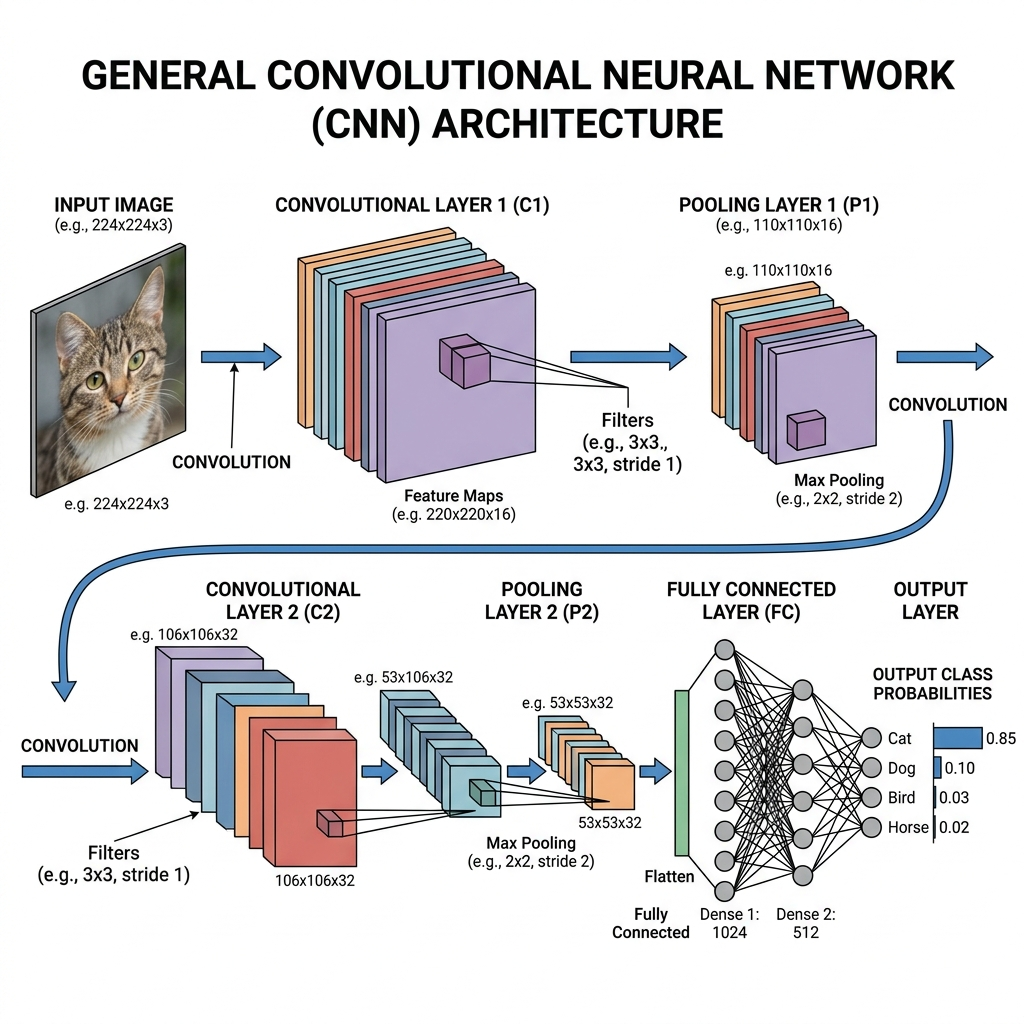
\includegraphics[width=0.85\textwidth]{cnn_general_arch.png}
    \caption{Sơ đồ kiến trúc tổng quan của mạng nơ-ron tích chập (CNN)}
    \label{fig:cnn_general_arch}
\end{figure}

Kiến trúc CNN tiêu chuẩn bao gồm ba cấu phần cơ bản xếp chồng tuần tự. Trước tiên là các lớp tích chập (Convolutional Layers) áp dụng các bộ lọc (kernel) trượt trên ảnh đầu vào để trích xuất đặc trưng cục bộ. Tiếp theo là các lớp gộp (Pooling Layers) có chức năng giảm kích thước không gian bản đồ đặc trưng bằng phép lấy cực đại (Max Pooling) hoặc trung bình (Average Pooling) nhằm giảm chi phí tính toán và tăng tính bất biến đối với các phép dịch chuyển nhỏ. Cuối cùng là các lớp kết nối đầy đủ (Fully Connected Layers) thực hiện kết hợp các đặc trưng đã trích xuất để phân loại cảm xúc.

Lịch sử phát triển của mạng CNN bắt nguồn từ mô hình Neocognitron đề xuất bởi Kunihiko Fukushima vào năm 1980, giới thiệu các khái niệm sơ khai về lớp trích xuất đặc trưng (S-cells) và lớp bất biến dịch chuyển (C-cells) dựa trên cấu trúc vỏ não thị giác của động vật. Đến năm 1998, Yann LeCun và cộng sự đã hiện thực hóa mô hình này thành kiến trúc LeNet-5 để nhận dạng chữ số viết tay trên séc ngân hàng, đặt nền móng chính thức cho cơ chế tích chập và gộp đặc trưng chia sẻ trọng số. Mặc dù đạt thành công lớn, CNN thời kỳ này bị giới hạn hiệu năng do thiếu tài nguyên tính toán và các kỹ thuật tối ưu hóa hiện đại. 

Bước ngoặt lịch sử diễn ra vào năm 2012 khi kiến trúc AlexNet \cite{krizhevsky2012} tận dụng sức mạnh tính toán song song của GPU để huấn luyện mạng CNN sâu hơn trên tập dữ liệu ImageNet khổng lồ. Kể từ đó, sự phát triển của CNN tăng tốc vượt bậc với sự ra đời của cơ chế kết nối tắt trong ResNet (2016) giúp khắc phục vấn đề triệt tiêu gradient khi mạng đạt độ sâu hàng trăm lớp, cơ chế liên kết dày đặc trong DenseNet (2017) giúp tăng cường tái sử dụng đặc trưng, kiến trúc tích chập tách biệt chiều sâu trong MobileNet (2018) tối ưu cho thiết bị di động, và phương pháp tỷ lệ hóa hỗn hợp trong EfficientNet (2019) giúp cân bằng tối ưu tài nguyên tính toán. Trong những năm gần đây, xu hướng nghiên cứu đang tiếp tục phát triển tới các mô hình kết hợp lai giữa CNN và Vision Transformer (ViT) nhằm khai thác đồng thời khả năng biểu diễn cục bộ của tích chập và khả năng thiết lập mối quan hệ toàn cục của cơ chế attention.

\subsection{AlexNet}

Kiến trúc AlexNet được Krizhevsky và cộng sự đề xuất vào năm 2012 \cite{krizhevsky2012} là một bước ngoặt vĩ đại của học sâu, bao gồm 5 lớp tích chập xếp chồng kết hợp với 3 lớp kết nối đầy đủ. Điểm nổi bật của AlexNet là việc áp dụng hàm kích hoạt ReLU để giải quyết vấn đề triệt tiêu gradient và kỹ thuật Dropout để chống quá khớp trên các lớp kết nối đầy đủ có số lượng tham số lớn. Sơ đồ kiến trúc tổng thể của AlexNet được minh họa chi tiết trong Hình~\ref{fig:alexnet_arch}.

\begin{figure}[H]
    \centering
    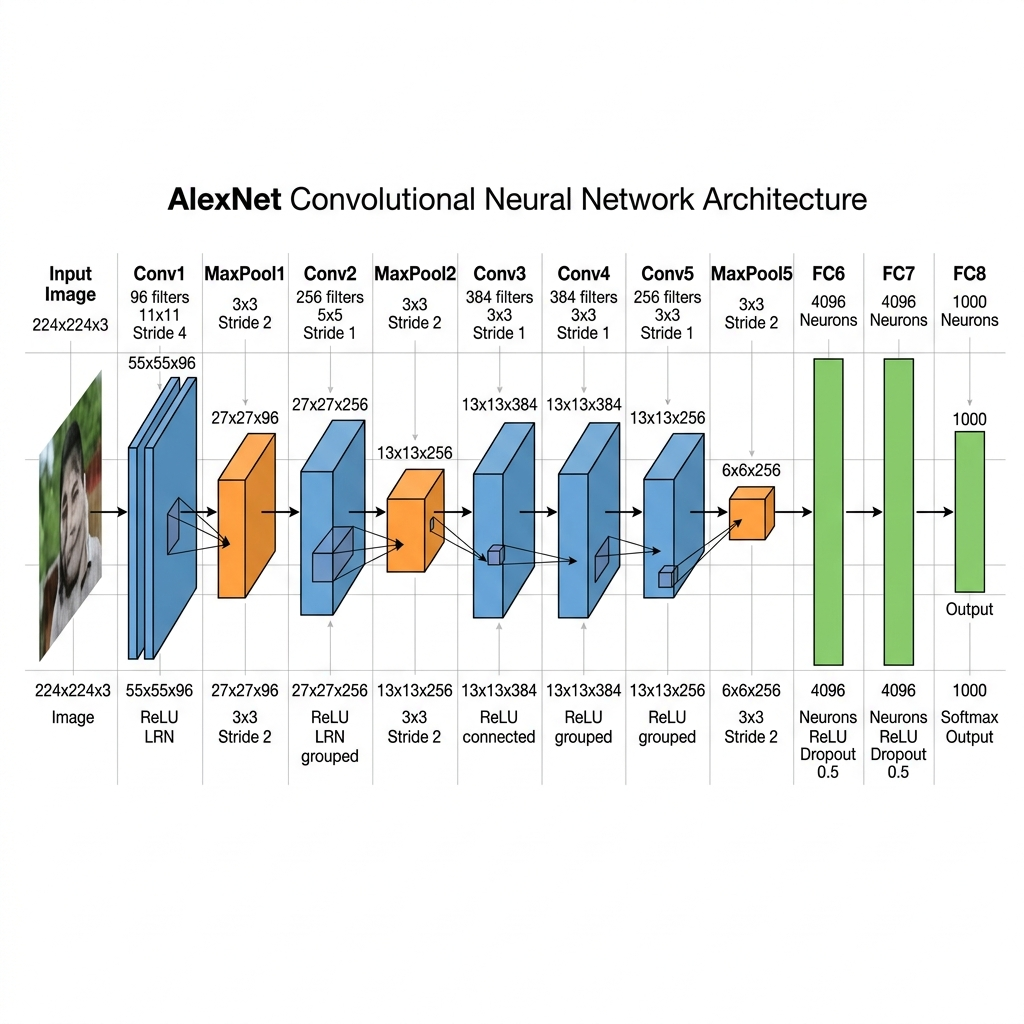
\includegraphics[width=0.85\textwidth]{alexnet_arch.png}
    \caption{Sơ đồ kiến trúc mạng nơ-ron tích chập AlexNet}
    \label{fig:alexnet_arch}
\end{figure}

Phân tích sơ đồ Hình~\ref{fig:alexnet_arch} cho thấy mô hình xử lý hình ảnh qua các khối tích chập lớn ở giai đoạn đầu để nắm bắt các đặc trưng hình học thô (như bộ lọc kích thước $11\times11$ ở lớp Conv1 và $5\times5$ ở lớp Conv2), sau đó giảm dần kích thước bộ lọc xuống $3\times3$ ở các lớp Conv3, Conv4 và Conv5 nhằm tinh chỉnh các đặc trưng ngữ nghĩa mức cao. Các lớp gộp cực đại (Max Pooling) được chèn xen kẽ để giảm độ phân giải không gian của bản đồ đặc trưng. Điểm yếu lớn của kiến trúc này nằm ở ba lớp kết nối đầy đủ (FC6, FC7, FC8) phía cuối, nơi chiếm tới hơn 90\% tổng số tham số của mô hình (tạo ra khoảng 57 triệu tham số), khiến mô hình cực kỳ nhạy cảm với hiện tượng quá khớp nếu dữ liệu huấn luyện không đủ lớn.

Trong nghiên cứu này, AlexNet đóng vai trò là mô hình baseline đối chứng với hai phiên bản triển khai cụ thể bao gồm AlexNet Finetuning và AlexNet GAP. Phiên bản AlexNet Finetuning giữ nguyên kiến trúc nguyên bản và chỉ thực hiện điều chỉnh số chiều đầu ra của lớp Fully Connected cuối cùng tương ứng với 4 lớp cảm xúc của bộ dữ liệu IEMOCAP, dẫn đến tổng số tham số lên tới 57,02 triệu. Cần chú ý rằng, mặc dù đầu vào phổ đồ trong đồ án là $256 \times 256$ pixels (vốn làm đầu ra của lớp tích chập Conv5 đạt kích thước $7 \times 7$ thay vì $6 \times 6$ như trong thiết kế ImageNet gốc), việc chuyển giao tri thức từ mô hình pre-trained vẫn thực hiện thành công nhờ việc tích hợp lớp gộp trung bình thích ứng (\texttt{nn.AdaptiveAvgPool2d((6, 6))}) chèn giữa phần trích xuất đặc trưng và bộ phân loại kết nối đầy đủ, giúp đồng bộ hóa kích thước tensor đầu vào cho lớp FC6 mà không làm đứt gãy hoặc yêu cầu tái cấu trúc các trọng số đã được học trước. 

Ngược lại, phiên bản cải tiến AlexNet GAP loại bỏ hoàn toàn các lớp Fully Connected nặng nề và thay thế bằng lớp gộp trung bình toàn cục (Global Average Pooling - GAP) kết hợp tích chập $1\times1$, giúp giảm số lượng tham số huấn luyện xuống chỉ còn 2,47 triệu (giảm 96\% so với nguyên bản) và hạn chế đáng kể hiện tượng quá khớp trên tập dữ liệu nhỏ của bài toán SER. Redesign này giúp cải thiện đáng kể khả năng tổng quát hóa trên dữ liệu kiểm thử.


\section{Transfer Learning}
\label{sec:transfer_learning}

Transfer Learning là kỹ thuật tận dụng trọng số đã được huấn luyện trước từ một tác vụ lớn (thường là ImageNet \cite{deng2009}) để chuyển giao tri thức sang một tác vụ mới có lượng dữ liệu hạn chế. Trong đồ án này, các mô hình CNN tiên tiến được khởi tạo bằng trọng số pre-trained ImageNet, sau đó thực hiện fine-tune trực tiếp trên phổ đồ Log-Spectrogram của dữ liệu IEMOCAP để nhận dạng cảm xúc.

\subsection{ResNet-18}

Mạng dư thừa (Residual Network - ResNet) do He và cộng sự phát triển năm 2016 \cite{he2016} đã giải quyết triệt để hiện tượng suy thoái hiệu năng mạng (degradation problem) khi tăng độ sâu. Cơ chế cốt lõi của ResNet là việc tích hợp các kết nối tắt (skip connection hoặc residual connection) cho phép thông tin đầu vào $\mathbf{x}$ bỏ qua một hoặc nhiều lớp tích chập và được cộng trực tiếp vào đầu ra của khối. Công thức toán học biểu diễn khối dư thừa cơ bản được xác định như sau:
\begin{equation}
    \mathbf{y} = \mathcal{F}(\mathbf{x}, \{W_i\}) + \mathbf{x}
    \label{eq:residual}
\end{equation}
Trong công thức này, $\mathbf{x}$ là đặc trưng đầu vào, $\mathbf{y}$ là đầu ra của khối, và $\mathcal{F}$ biểu thị ánh xạ dư thừa cần được tối ưu hóa. Kết nối tắt giúp gradient lan truyền ngược dễ dàng qua các lớp mà không bị triệt tiêu (gradient vanishing). Phiên bản ResNet-18 có 18 lớp trọng số cấu tạo từ các khối BasicBlock (hai lớp tích chập $3\times3$ kết hợp với Batch Normalization và ReLU). Cấu trúc chi tiết của khối dư thừa được minh họa trong Hình~\ref{fig:resnet_arch}.

\begin{figure}[H]
    \centering
    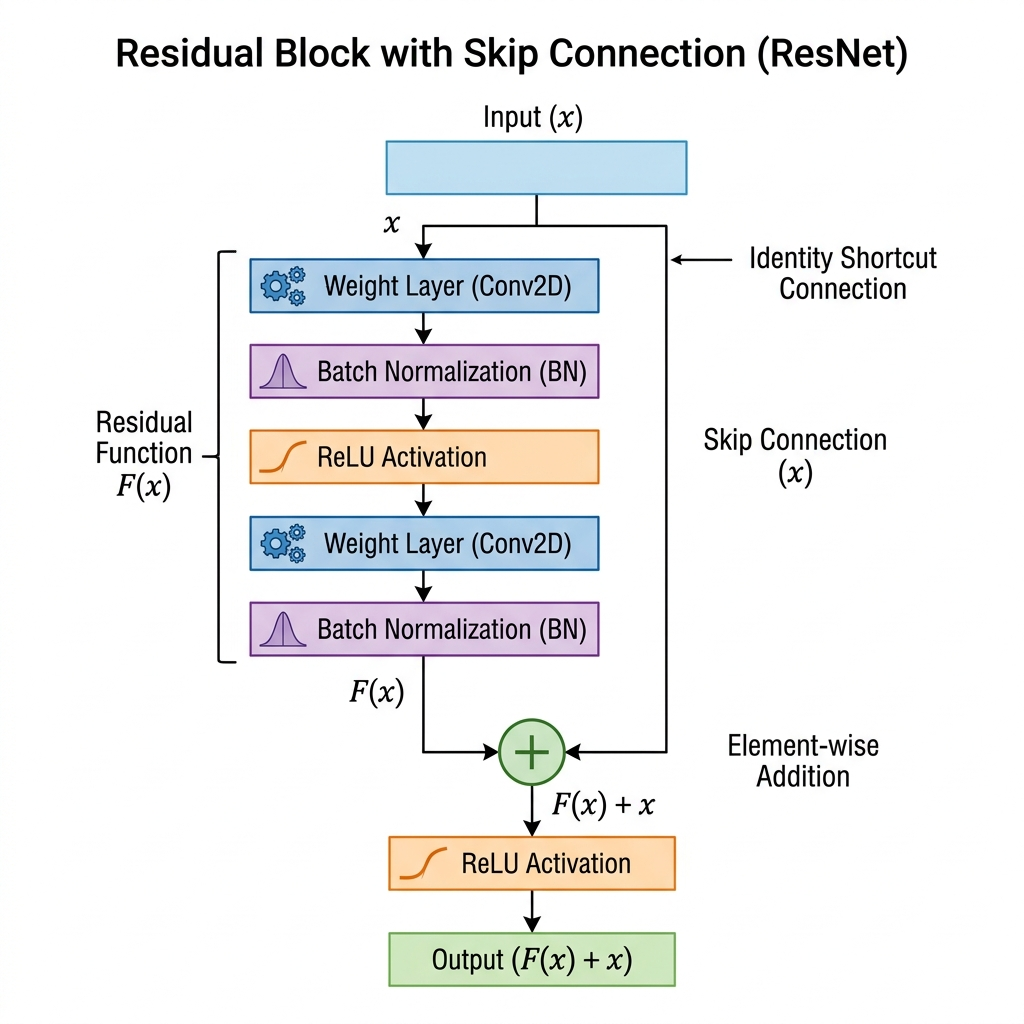
\includegraphics[width=0.55\textwidth]{resnet_arch.png}
    \caption{Kiến trúc khối dư thừa (Residual Block) với kết nối tắt trong ResNet}
    \label{fig:resnet_arch}
\end{figure}

Dựa vào sơ đồ Hình~\ref{fig:resnet_arch}, đặc trưng đầu vào $\mathbf{x}$ đi qua hai nhánh song song. Nhánh thứ nhất thực hiện trích xuất thông qua hai lớp trọng số tích chập liên tiếp (kèm chuẩn hóa Batch Normalization và hàm kích hoạt ReLU). Nhánh thứ hai là kết nối tắt (Identity Shortcut) truyền trực tiếp $\mathbf{x}$ mà không chịu bất kỳ biến đổi phi tuyến tính nào. Hai nhánh sau đó được cộng chập trực tiếp trước khi đi qua lớp kích hoạt ReLU cuối cùng của khối. Trong trường hợp kích thước kênh hoặc độ phân giải không gian của $\mathbf{x}$ thay đổi giữa đầu vào và đầu ra, nhánh shortcut sẽ áp dụng một phép tích chập $1\times1$ để điều chỉnh số chiều tương thích. Thiết kế này giúp gradient trong quá trình lan truyền ngược có thể truyền thẳng qua nhánh shortcut mà không bị triệt tiêu bởi các phép nhân ma trận trọng số, cho phép mạng đạt độ sâu hàng trăm lớp một cách ổn định. Tổng số tham số của ResNet-18 là 11,18 triệu, cung cấp khả năng biểu diễn đặc trưng mạnh mẽ cho phổ đồ âm thanh.

\subsection{DenseNet-121}

Mạng tích chập kết nối dày đặc (DenseNet) do Huang và cộng sự đề xuất năm 2017 \cite{huang2017} đưa ra giải pháp kết nối trực tiếp tất cả các lớp với nhau trong một khối liên kết dày đặc (Dense Block). Thay vì thực hiện phép cộng đặc trưng như ResNet, mỗi lớp trong DenseBlock sẽ nhận bản đồ đặc trưng của toàn bộ các lớp phía trước làm đầu vào thông qua phép ghép nối (concatenation) theo chiều kênh:
\begin{equation}
    \mathbf{x}_l = H_l\left([\mathbf{x}_0, \mathbf{x}_1, \ldots, \mathbf{x}_{l-1}]\right)
    \label{eq:densenet}
\end{equation}
Trong đó, $[\mathbf{x}_0, \mathbf{x}_1, \ldots, \mathbf{x}_{l-1}]$ biểu diễn phép ghép bản đồ đặc trưng được tạo ra bởi các lớp trước đó, và $H_l$ là phép biến đổi phi tuyến tính. Cơ chế này giúp cải thiện đáng kể luồng thông tin và gradient trong mạng, khuyến khích tái sử dụng đặc trưng và giảm thiểu số tham số thực tế cần huấn luyện do các lớp không cần học lại đặc trưng trùng lặp. Giữa các khối Dense Block, mạng sử dụng các lớp chuyển tiếp (Transition Layers) gồm tích chập $1\times1$ và gộp trung bình $2\times2$. Sơ đồ khối liên kết dày đặc được biểu diễn trong Hình~\ref{fig:densenet_arch}.

\begin{figure}[H]
    \centering
    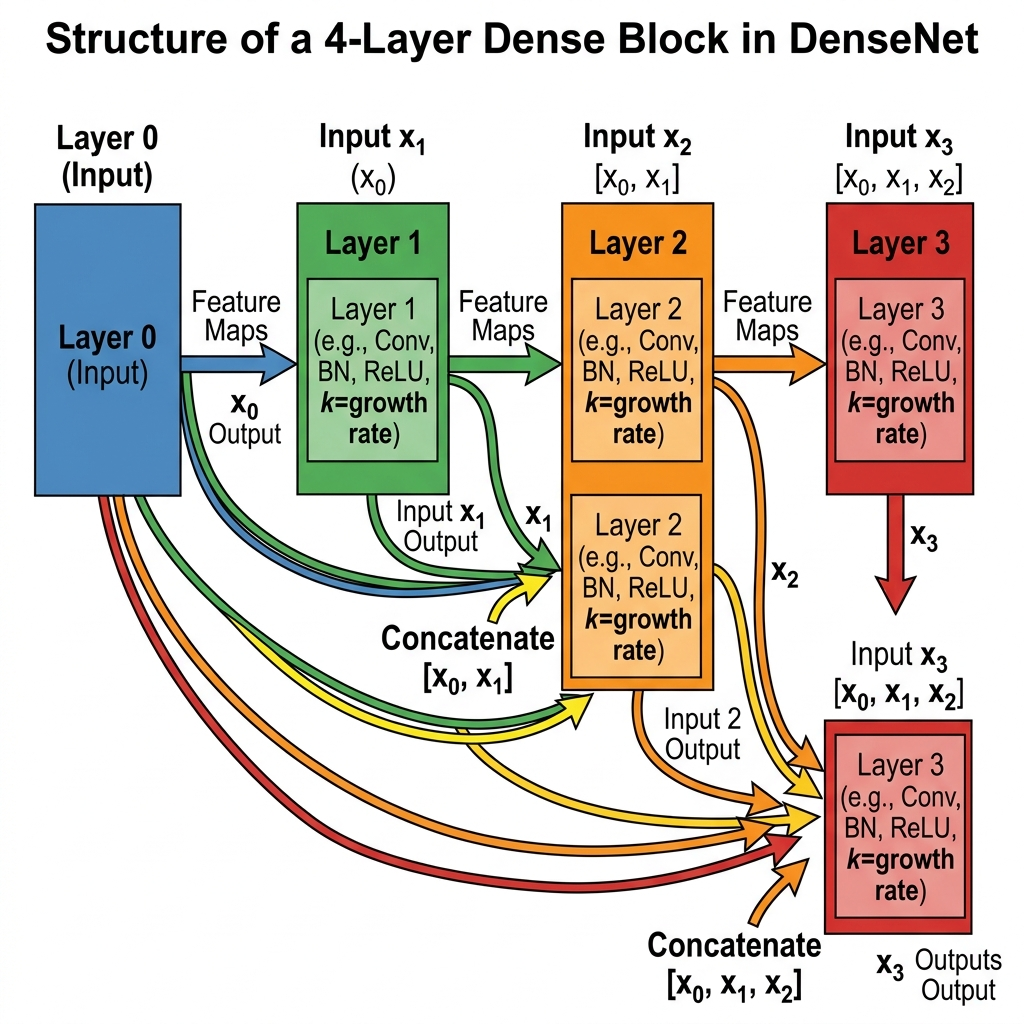
\includegraphics[width=0.75\textwidth]{densenet_arch.png}
    \caption{Sơ đồ liên kết dày đặc (Dense Block) trong kiến trúc DenseNet}
    \label{fig:densenet_arch}
\end{figure}

Phân tích sơ đồ Hình~\ref{fig:densenet_arch} cho thấy cấu trúc dòng chảy thông tin cực kỳ cấu trúc: Layer $H_1$ nhận đầu vào từ Layer $0$; Layer $H_2$ nhận đầu vào từ cả Layer $0$ và đặc trưng trích xuất của Layer $1$ sau khi ghép kênh; quá trình này tiếp diễn tuần tự cho đến Layer cuối cùng. Tham số growth rate ($k=32$) quy định số lượng kênh đặc trưng mới được tạo ra ở mỗi bước biến đổi. Thiết kế ghép kênh thay vì cộng chập giúp mô hình giữ lại toàn vẹn các thông tin tần số thấp và tần số cao được học từ các lớp trước đó mà không bị mờ nhòe đặc trưng, tối ưu hóa việc phân tách các đặc trưng âm học nhạy cảm. Kiến trúc DenseNet-121 gồm 121 lớp với tổng số 6,96 triệu tham số giúp khai thác triệt để các đặc trưng âm học ở nhiều cấp độ phân giải.

\subsection{EfficientNet-B0}

Mạng EfficientNet do Tan và Lê đề xuất năm 2019 \cite{tan2019} tối ưu hóa hiệu năng CNN một cách có hệ thống thông qua kỹ thuật tỷ lệ hóa hỗn hợp (Compound Scaling). Thay vì tăng riêng lẻ độ sâu, chiều rộng hoặc độ phân giải ảnh đầu vào, phương pháp này tỷ lệ hóa đồng đều cả ba chiều bằng một hệ số tỷ lệ $\phi$ cố định duy nhất:
\begin{equation}
    \text{depth}: d = \alpha^\phi, \quad \text{width}: w = \beta^\phi, \quad \text{resolution}: r = \gamma^\phi
    \label{eq:efficientnet}
\end{equation}
với ràng buộc $\alpha \cdot \beta^2 \cdot \gamma^2 \approx 2$ nhằm đảm bảo khi tăng $\phi$, lượng FLOPS yêu cầu tăng tuyến tính theo mức $2^\phi$. Khối MBConv (Mobile Inverted Bottleneck Convolution) là thành phần cấu tạo chính của EfficientNet, tích hợp tích chập tách biệt chiều sâu (depthwise separable convolution) kết hợp với khối chú ý Squeeze-and-Excitation (SE) giúp mô hình tự học trọng số biểu thị tầm quan trọng của từng kênh đặc trưng. Sơ đồ khối MBConv được minh họa trong Hình~\ref{fig:efficientnet_arch}.

\begin{figure}[H]
    \centering
    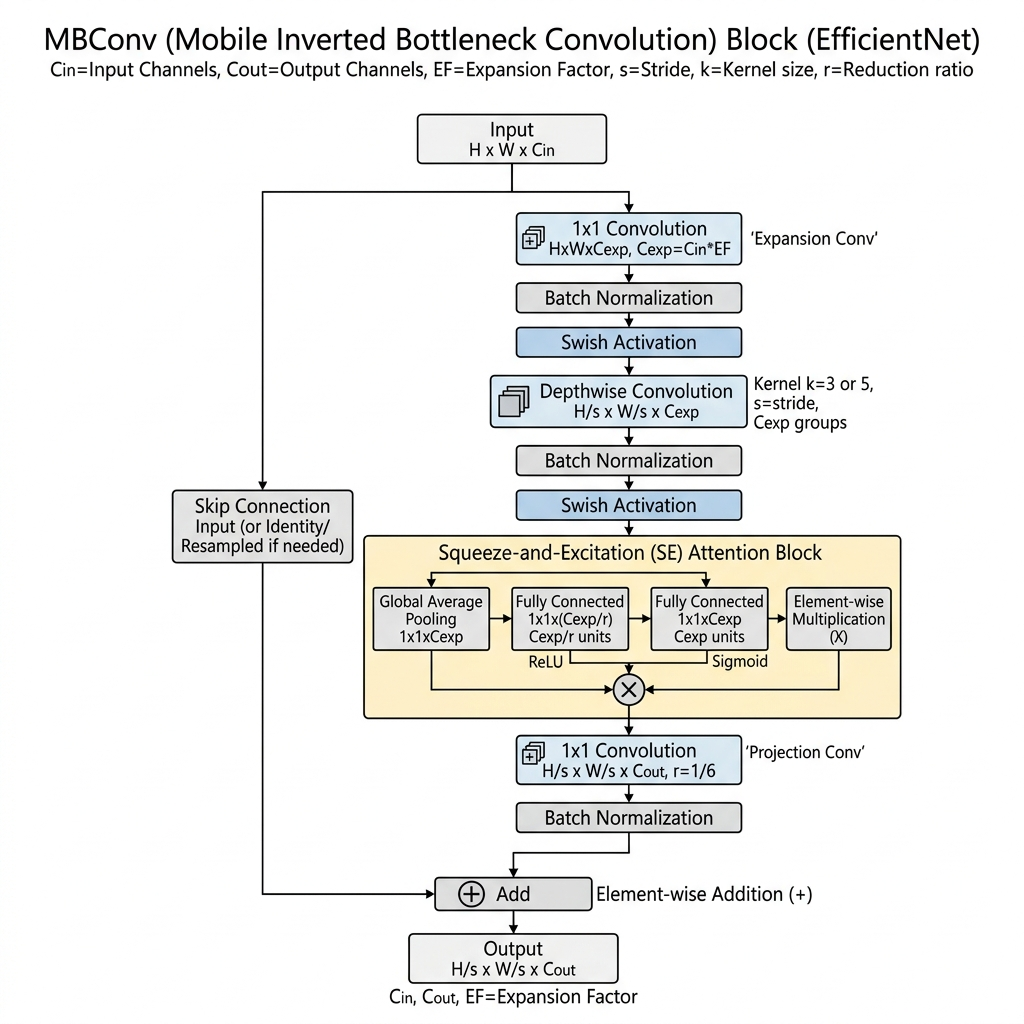
\includegraphics[width=0.8\textwidth]{efficientnet_arch.png}
    \caption{Kiến trúc khối MBConv tích hợp cơ chế chú ý Squeeze-and-Excitation trong EfficientNet}
    \label{fig:efficientnet_arch}
\end{figure}

Sơ đồ Hình~\ref{fig:efficientnet_arch} mô tả chi tiết luồng xử lý của khối MBConv. Đặc trưng đầu vào trước hết được mở rộng số kênh qua lớp tích chập $1\times1$ để chuyển sang không gian đặc trưng số chiều lớn, sau đó đi qua lớp tích chập tách biệt chiều sâu (Depthwise Conv) kích thước $3\times3$ hoặc $5\times5$ để học các thông tin không gian cục bộ một cách tiết kiệm chi phí tính toán. Đặc trưng tiếp tục đi qua khối Squeeze-and-Excitation (SE) thực hiện ép kênh qua Global Average Pooling và tái khôi phục qua hai lớp Fully Connected để tạo ra trọng số chú ý cho từng kênh, nhân trực tiếp vào đặc trưng nhằm làm nổi bật các kênh tần số âm thanh quan trọng. Cuối cùng, lớp chiếu $1\times1$ hạ số chiều kênh về mức ban đầu và được cộng chập với shortcut từ đầu vào. Thiết kế MBConv giúp EfficientNet-B0 (4,01 triệu tham số) đạt hiệu năng cao nhất với chi phí tính toán tối thiểu trên phổ đồ giọng nói.

\subsection{MobileNet-V2}

MobileNet-V2 được Sandler và cộng sự giới thiệu vào năm 2018 \cite{sandler2018} là một kiến trúc CNN gọn nhẹ được tối ưu hóa cho các ứng dụng chạy trên thiết bị di động và hệ thống nhúng. Mô hình sử dụng tích chập tách biệt theo chiều sâu (depthwise separable convolution) để phân tách phép tích chập thông thường thành hai bước tích chập độc lập gồm depthwise convolution và pointwise convolution, giúp giảm mạnh số lượng phép tính. MobileNet-V2 giới thiệu khối nghịch đảo residual (Inverted Residual Block) thực hiện mở rộng số kênh ở lớp giữa và chiếu giảm số kênh ở đầu ra thông qua lớp cổ chai tuyến tính (Linear Bottleneck) không sử dụng hàm kích hoạt phi tuyến tính nhằm tránh mất mát thông tin hữu ích trong không gian số chiều thấp. Cấu trúc khối Inverted Residual được thể hiện trong Hình~\ref{fig:mobilenet_arch}.

\begin{figure}[H]
    \centering
    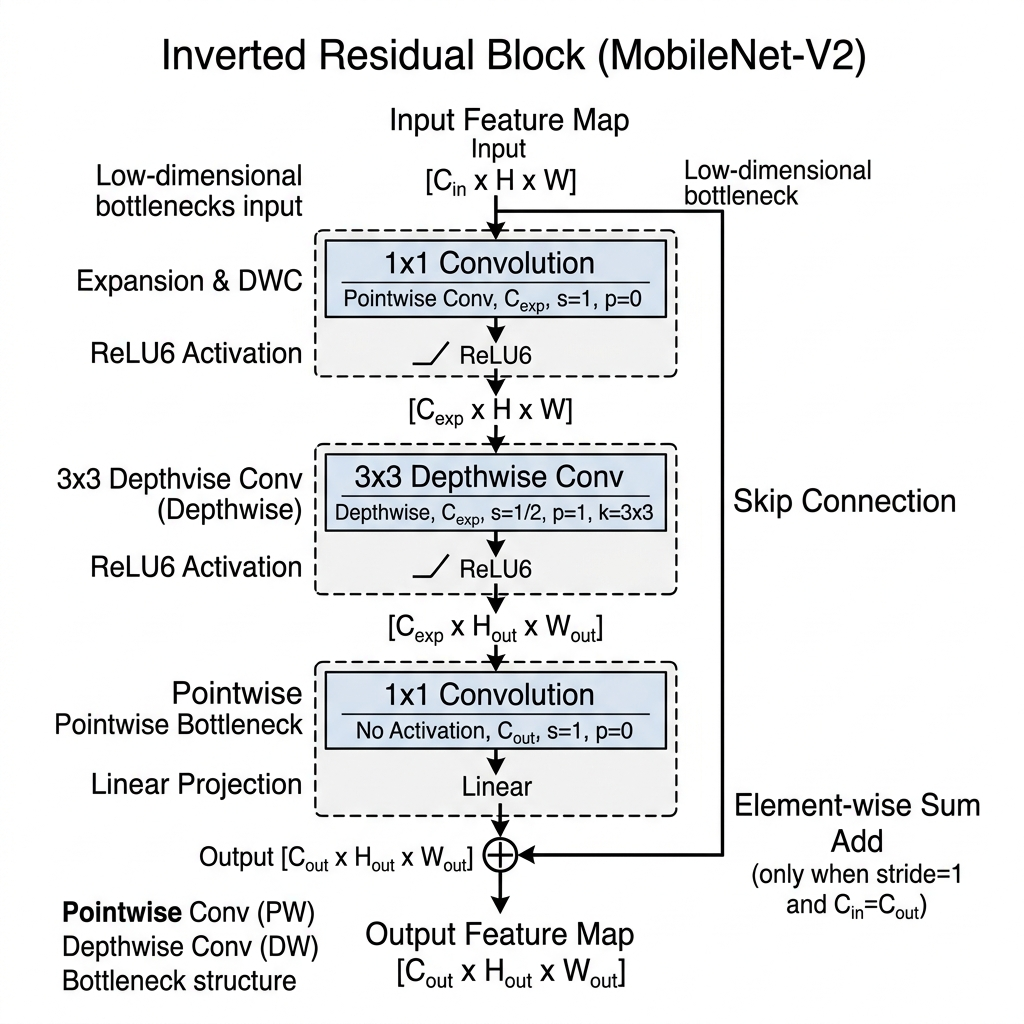
\includegraphics[width=0.8\textwidth]{mobilenet_arch.png}
    \caption{Kiến trúc khối nghịch đảo residual (Inverted Residual Block) và Linear Bottleneck trong MobileNet-V2}
    \label{fig:mobilenet_arch}
\end{figure}

Phân tích Hình~\ref{fig:mobilenet_arch} làm rõ sự khác biệt giữa Inverted Residual và Residual Block thông thường. Thay vì kết nối các lớp có số lượng kênh lớn, nhánh shortcut của MobileNet-V2 kết nối trực tiếp giữa các lớp cổ chai tuyến tính (Linear Bottleneck) có số lượng kênh rất nhỏ (không gian số chiều thấp). Trong khối, đặc trưng trước tiên được mở rộng kênh lên gấp 6 lần (Expansion Layer), sau đó trích xuất không gian bằng tích chập tách biệt chiều sâu (Depthwise Convolution), và cuối cùng chiếu giảm số kênh (Projection Layer) sử dụng hàm kích hoạt tuyến tính (Linear Activation) thay vì ReLU. Thiết kế Linear Bottleneck cực kỳ quan trọng vì hàm ReLU trong không gian số chiều thấp có xu hướng triệt tiêu hoàn toàn các giá trị âm, làm mất mát nghiêm trọng thông tin đặc trưng; việc giữ kích hoạt tuyến tính ở đầu ra lớp cổ chai giúp duy trì nguyên vẹn các đặc trưng âm học nhạy cảm. Với chỉ 2,23 triệu tham số, MobileNet-V2 đáp ứng khả năng tính toán thời gian thực trên các phần cứng cấu hình yếu.


\section{Hàm lỗi Focal Loss}
\label{sec:focal_loss}

Hàm lỗi Cross Entropy truyền thống xử lý mọi mẫu dữ liệu một cách đồng đều:
\begin{equation}
    \text{CE}(p_t) = -\log(p_t)
    \label{eq:ce}
\end{equation}
Điều này dẫn đến việc mô hình dễ bị chi phối bởi lớp đa số (Neutral) trong môi trường dữ liệu mất cân bằng nghiêm trọng. Nhằm khắc phục hạn chế này, Focal Loss \cite{lin2017} giới thiệu thêm một hệ số điều chỉnh động $(1 - p_t)^\gamma$ vào công thức tính lỗi:
\begin{equation}
    \text{FL}(p_t) = -\alpha_t \cdot (1 - p_t)^\gamma \cdot \log(p_t)
    \label{eq:focal}
\end{equation}
Trong công thức trên, $p_t$ đại diện cho xác suất dự đoán đúng của mô hình đối với lớp thực tế; $\gamma \geq 0$ là hệ số tập trung (focusing parameter) dùng để điều khiển tốc độ giảm trọng số lỗi đối với các mẫu dễ phân loại (trong đồ án sử dụng giá trị tối ưu $\gamma = 2.0$); và $\alpha_t$ là hệ số cân bằng lớp. Cần lưu ý rằng trong bài báo gốc của Lin và cộng sự \cite{lin2017}, Focal Loss được thiết kế ban đầu cho bài toán phân loại nhị phân với $\alpha \in [0, 1]$ là một siêu tham số cố định được điều chỉnh thủ công. Để phù hợp với bài toán phân loại đa lớp thực tế trong đồ án này, hệ số $\alpha_t$ được triển khai dưới dạng một cơ chế gán trọng số lớp động (class weighting scheme) dựa trên nghịch đảo tần suất của từng lớp trong tập huấn luyện:
\begin{equation}
    \alpha_c = \frac{N_{\text{total}}}{C \times N_c}
\end{equation}
trong đó $N_c$ là số mẫu của lớp $c$, $C$ là tổng số lớp ($C = 4$), và $N_{\text{total}}$ là tổng số mẫu của tất cả các lớp trong tập huấn luyện. Cơ chế điều chỉnh động này giúp giảm mạnh phần đóng góp lỗi từ các mẫu đã phân loại đúng và buộc mô hình tập trung tối ưu hóa trên các mẫu khó thuộc lớp thiểu số (như Happiness, Anger).


\section{Kỹ thuật tăng cường dữ liệu EMix}
\label{sec:emix}

EMix (Emotion-aware Mixup) \cite{dang2023emix} là kỹ thuật tăng cường dữ liệu dựa trên nền tảng của thuật toán MixUp truyền thống \cite{zhang2018}, được thiết kế chuyên biệt cho bài toán nhận dạng cảm xúc giọng nói (SER). Thay vì thực hiện trộn ngẫu nhiên hai mẫu bất kỳ tạo ra các nhãn mập mờ làm mờ ranh giới cảm xúc, EMix đề xuất các chiến lược trộn có kiểm soát dựa trên nhãn cảm xúc thực tế.

Chiến lược thứ nhất là EMix-S (Same-class Mixup), thực hiện trộn tuyến tính hai mẫu âm thanh có cùng nhãn cảm xúc để củng cố ranh giới và tính phân tách của từng lớp. Công thức toán học trộn được biểu diễn:
\begin{equation}
    \tilde{x}_i = \lambda \cdot x_i + (1 - \lambda) \cdot x_j, \quad \text{với } y_i = y_j, \quad \lambda \sim U(0, 1)
    \label{eq:emix_s}
\end{equation}
Trong đó, hai phổ đồ $x_i$ và $x_j$ có cùng nhãn cảm xúc ($y_i = y_j$) được trộn với nhau thông qua trọng số $\lambda$ được lấy ngẫu nhiên từ phân phối đều $U(0, 1)$, và nhãn đầu ra cho mẫu mới được giữ nguyên là $\tilde{y}_i = y_i$.

Chiến lược thứ hai là EMix-N (Neutral Mixup), thực hiện trộn mẫu cảm xúc mục tiêu với một mẫu cảm xúc trung tính (Neutral) đóng vai trò như một dạng nhiễu nền tự nhiên. Phép trộn này giúp mô hình nhận diện tốt hơn các đặc trưng cảm xúc ngay cả khi bị suy hao hoặc bị lấn át bởi trạng thái nói bình thường. Công thức cụ thể là:
\begin{equation}
    \tilde{x}_i = \lambda \cdot x_i + (1 - \lambda) \cdot x_{\text{neu}}, \quad \lambda \sim U(0.5, 1.0)
    \label{eq:emix_n}
\end{equation}
Với hệ số $\lambda \geq 0.5$ nhằm đảm bảo đặc trưng cảm xúc mục tiêu vẫn chiếm ưu thế ngữ nghĩa so với mẫu Neutral, và nhãn đích đầu ra vẫn được duy trì theo mẫu cảm xúc mục tiêu.

Chiến lược cuối cùng là EMix-NS (Combined) đại diện cho phương pháp kết hợp đồng thời cả hai chiến lược trên. Với mỗi mini-batch trong quá trình huấn luyện, thuật toán sẽ ngẫu nhiên lựa chọn thực hiện EMix-N hoặc EMix-S với xác suất đồng đều ($p = 0.5$). Sự kết hợp này mang lại dải biến thể phong phú cho tập dữ liệu huấn luyện, giúp mô hình cải thiện tối đa tính tổng quát.


% ====== CHƯƠNG 3: PHƯƠNG PHÁP ĐỀ XUẤT ======
% ============================================================
% CHƯƠNG 3: PHƯƠNG PHÁP ĐỀ XUẤT
% ============================================================
\chapter{Phương pháp đề xuất}
\label{chap:methodology}

\section{Tổng quan hệ thống}
\label{sec:system_overview}

Hệ thống nhận dạng cảm xúc giọng nói được xây dựng gồm ba giai đoạn xử lý cốt lõi liên kết chặt chẽ với nhau: (1) Trích xuất đặc trưng từ tín hiệu âm thanh thô thành ma trận Log-Spectrogram, (2) Tiền xử lý dữ liệu và chuẩn hóa dạng ảnh đầu vào, và (3) Huấn luyện và phân loại cảm xúc bằng các kiến trúc CNN tiên tiến. Sơ đồ tổng quan mô tả chi tiết luồng xử lý và mối liên hệ giữa các giai đoạn được thể hiện trong Hình~\ref{fig:system_pipeline}.

\begin{figure}[H]
    \centering
    \resizebox{\textwidth}{!}{%
    \begin{tikzpicture}[
        node distance=0.6cm and 0.4cm,
        block/.style={
            draw,
            rectangle,
            rounded corners=4pt,
            align=center,
            fill=white,
            draw=blue!60!black,
            font=\small,
            minimum height=1.1cm,
            minimum width=2.4cm,
            thick
        },
        input/.style={
            draw,
            rectangle,
            rounded corners=6pt,
            align=center,
            fill=green!5,
            draw=green!50!black,
            font=\small\bfseries,
            minimum height=1.1cm,
            minimum width=2.2cm,
            thick
        },
        data/.style={
            draw,
            rectangle,
            align=center,
            fill=yellow!5,
            draw=yellow!50!black,
            font=\small,
            minimum height=1.1cm,
            minimum width=2.2cm,
            thick
        },
        output/.style={
            draw,
            rectangle,
            rounded corners=6pt,
            align=center,
            fill=red!5,
            draw=red!50!black,
            font=\small\bfseries,
            minimum height=1.1cm,
            minimum width=2.2cm,
            thick
        },
        arrow/.style={
            ->,
            >=stealth,
            thick,
            draw=black!70
        },
        stagebox/.style={
            draw=gray!30,
            fill=gray!5,
            rounded corners=8pt,
            inner sep=10pt,
            thick
        }
    ]
        % Giai đoạn 1: Trích xuất đặc trưng
        \node (audio) [input] {Tín hiệu .wav\\(16 kHz)};
        \node (preemp) [block, right=of audio] {Bộ lọc tiền nhấn\\(Pre-emphasis)};
        \node (stft) [block, right=of preemp] {Biến đổi STFT\\(Cửa sổ Hamming)};
        \node (log) [block, right=of stft] {Log-scale (dB)\\200 băng tần};
        \node (spec) [data, right=of log] {Log-Spectrogram\\($200 \times T$)};
        
        \begin{scope}[on background layer]
            \node (stage1) [stagebox, fit=(audio) (spec), label={[font=\small\bfseries\color{blue!80!black}]above:GIAI ĐOẠN 1: TRÍCH XUẤT ĐẶC TRƯNG (FEATURE EXTRACTION)}] {};
        \end{scope}

        % Giai đoạn 2: Tiền xử lý dữ liệu
        \node (seg) [block, below=of audio, yshift=-1.8cm] {Phân đoạn \& Đệm\\($200 \times 300$)};
        \node (norm) [block, right=of seg] {MinMax \& 3-ch\\(Pseudo-RGB)};
        \node (resize) [block, right=of norm] {Resize \& Z-Score\\($3 \times 256 \times 256$)};
        
        \begin{scope}[on background layer]
            \node (stage2) [stagebox, fit=(seg) (resize), label={[font=\small\bfseries\color{blue!80!black}]above:GIAI ĐOẠN 2: TIỀN XỬ LÝ (PREPROCESSING)}] {};
        \end{scope}

        % Giai đoạn 3: Huấn luyện & Phân loại
        \node (cnn) [block, right=of resize, xshift=1.2cm] {Huấn luyện CNN\\(Transfer Learning)};
        \node (output) [output, right=of cnn] {Phân loại\\4 cảm xúc};
        
        \begin{scope}[on background layer]
            \node (stage3) [stagebox, fit=(cnn) (output), label={[font=\small\bfseries\color{blue!80!black}]above:GIAI ĐOẠN 3: PHÂN LOẠI (CLASSIFICATION)}] {};
        \end{scope}

        % Connections
        \draw [arrow] (audio) -- (preemp);
        \draw [arrow] (preemp) -- (stft);
        \draw [arrow] (stft) -- (log);
        \draw [arrow] (log) -- (spec);
        \draw [arrow] (spec.south) -- ++(0,-0.8) -| (seg.north);
        \draw [arrow] (seg) -- (norm);
        \draw [arrow] (norm) -- (resize);
        \draw [arrow] (resize.east) -- (cnn.west);
        \draw [arrow] (cnn) -- (output);
    \end{tikzpicture}%
    }
    \caption{Sơ đồ tổng quan phân chia luồng xử lý dữ liệu và huấn luyện hệ thống theo các giai đoạn cụ thể}
    \label{fig:system_pipeline}
\end{figure}

Luồng xử lý dữ liệu đầy đủ của hệ thống được mô tả theo sơ đồ toán học như sau:
\begin{equation*}
\text{.wav (16kHz)} \xrightarrow{\text{Pre-emphasis}} x_{\text{flt}}(t) \xrightarrow{\text{STFT}} A(f, t) \xrightarrow{\text{Log (dB)}} S_{\text{dB}}(200 \times T)
\end{equation*}
\begin{equation*}
\xrightarrow{\text{Segment + Pad}} (200 \times 300) \xrightarrow{\text{Normalize + 3ch}} (3 \times 200 \times 300) \xrightarrow{\text{Resize + Z-Score}} (3 \times 256 \times 256)
\end{equation*}


\section{Bộ dữ liệu IEMOCAP}
\label{sec:iemocap_dataset}

\subsection{Giới thiệu}

Bộ dữ liệu \textbf{IEMOCAP (Interactive Emotional Dyadic Motion Capture)} được xây dựng và thu thập bởi phòng thí nghiệm SAIL (Speech Analysis and Interpretation Laboratory) thuộc Đại học Nam California (USC), công bố chính thức vào năm 2008 \cite{busso2008}. Đây là một trong những cơ sở dữ liệu đa phương thức quy chuẩn và được trích dẫn rộng rãi nhất trên thế giới dùng để nghiên cứu nhận dạng cảm xúc tự động. Về thiết lập ghi hình, bộ dữ liệu sử dụng hệ thống bắt chuyển động cơ thể hiện đại (motion capture) để thu thập các biểu cảm vật lý thông qua các điểm đánh dấu (markers) trên khuôn mặt, đầu và tay của diễn viên, đồng thời thu lại tín hiệu âm thanh chất lượng cao (tần số lấy mẫu 16 kHz, định dạng 16-bit mono) thông qua microphone đeo tai riêng biệt cho từng người. Quy mô dữ liệu đạt khoảng 12 giờ dữ liệu thô, được thực hiện bởi 10 diễn viên chuyên nghiệp thuộc đoàn kịch Đại học (gồm 5 nam và 5 nữ) chia làm 5 cặp đối thoại song song tương ứng với 5 phiên hội thoại (Session 1 đến Session 5).

Để kích hoạt các phản ứng cảm xúc tự nhiên nhất, các diễn viên thực hiện các buổi diễn đôi (dyadic interactions) dựa trên hai kịch bản thiết kế sẵn. Thứ nhất là kịch bản hội thoại ngẫu hứng (improvised sessions), nơi các diễn viên được cung cấp một tình huống giả lập cụ thể (ví dụ: tranh cãi về một hóa đơn thanh toán sai, nhận được tin vui trúng tuyển công việc mơ ước, mất đồ đạc cá nhân quan trọng, hoặc đối diện với tin buồn từ gia đình) và tự do đối thoại ngẫu hứng nhằm bộc lộ cảm xúc chân thực nhất mà không theo bất kỳ kịch bản viết sẵn nào. Thứ hai là kịch bản diễn theo lời thoại (scripted sessions), nơi các diễn viên đọc và biểu diễn trực tiếp theo một kịch bản thoại cố định được thiết kế để chứa đựng các từ ngữ mang xu hướng cảm xúc mạnh.

Về quy trình gán nhãn và đánh giá cảm xúc (Annotation), mỗi câu nói (utterance) sau khi cắt phân đoạn được đánh giá bởi ít nhất 3 chuyên gia gán nhãn là con người. Các chuyên gia tiến hành đánh giá cảm xúc theo hai giao thức song song bao gồm gán nhãn phân loại cảm xúc rời rạc (gồm các lớp: Anger, Sadness, Happiness, Neutral, Excitement, Fear, Frustration, Surprise, và Other) và đánh giá các thuộc tính cảm xúc đa chiều trên thang điểm từ 1 đến 5 (bao gồm Valence biểu thị mức độ tích cực/tiêu cực, Activation biểu thị mức độ kích hoạt năng lượng âm học, và Dominance biểu thị mức độ làm chủ tình huống). Nhãn cảm xúc rời rạc cuối cùng của từng câu nói được xác định dựa trên biểu quyết đa số (majority vote) của các chuyên gia. Nếu không có sự đồng thuận tối thiểu của 2 trên 3 chuyên gia, câu nói đó sẽ bị gán nhãn không xác định (xxx) và bị loại bỏ khỏi các nghiên cứu tiêu chuẩn. Trong đồ án này, nhóm nghiên cứu tập trung trích xuất kênh tín hiệu âm thanh của toàn bộ các phiên hội thoại ngẫu hứng để đảm bảo tính tự nhiên tối đa của ngữ điệu giọng nói, đồng thời lọc lấy các câu nói đạt sự đồng thuận cao thuộc 4 lớp cảm xúc chính gồm Anger, Sadness, Happiness và Neutral để làm tập dữ liệu huấn luyện.

\subsection{Lọc dữ liệu}

Để đảm bảo tính tự nhiên và sự tập trung của mô hình, dữ liệu được lọc theo các tiêu chí nghiêm ngặt. Trước hết, đồ án chỉ khai thác dữ liệu hội thoại ngẫu hứng (improvised) để phản ánh chân thực cao độ và ngữ điệu tự nhiên của giọng nói trong giao tiếp thực tế. Tiếp theo, hệ thống tiến hành lọc và chỉ giữ lại 4 lớp cảm xúc chính bao gồm Anger (Tức giận), Sadness (Buồn bã), Happiness (Vui vẻ) và Neutral (Bình thường), loại bỏ hoàn toàn các nhãn không đạt đồng thuận cao hoặc thuộc các trạng thái cảm xúc khác. Cuối cùng, đồ án quyết định giữ nguyên sự độc lập của nhãn Happiness mà không gộp chung với lớp Excited, làm tăng tính thách thức và độ khách quan cho bài toán phân loại.

\subsection{Thống kê dữ liệu sau lọc}

Sau khi lọc, tổng số câu nói thu được là \textbf{2.280 câu}. Sự phân bổ cụ thể của các mẫu theo nhãn cảm xúc được tổng hợp trong Bảng~\ref{tab:data_distribution}.

\begin{table}[H]
\centering
\caption{Thống kê phân bổ mẫu theo nhãn cảm xúc (cấp câu nói)}
\label{tab:data_distribution}
\begin{tabular}{lccc}
\toprule
\textbf{Nhãn cảm xúc} & \textbf{Số câu nói} & \textbf{Tỉ lệ (\%)} & \textbf{Vai trò} \\
\midrule
Neutral (Bình thường) & 1.099 & 48,2 & Lớp đa số \\
Sadness (Buồn bã) & 608 & 26,7 & -- \\
Anger (Tức giận) & 289 & 12,7 & Lớp thiểu số \\
Happiness (Vui vẻ) & 284 & 12,5 & Lớp thiểu số nhất \\
\midrule
\textbf{Tổng cộng} & \textbf{2.280} & \textbf{100,0} & \\
\bottomrule
\end{tabular}
\end{table}

\begin{figure}[H]
    \centering
    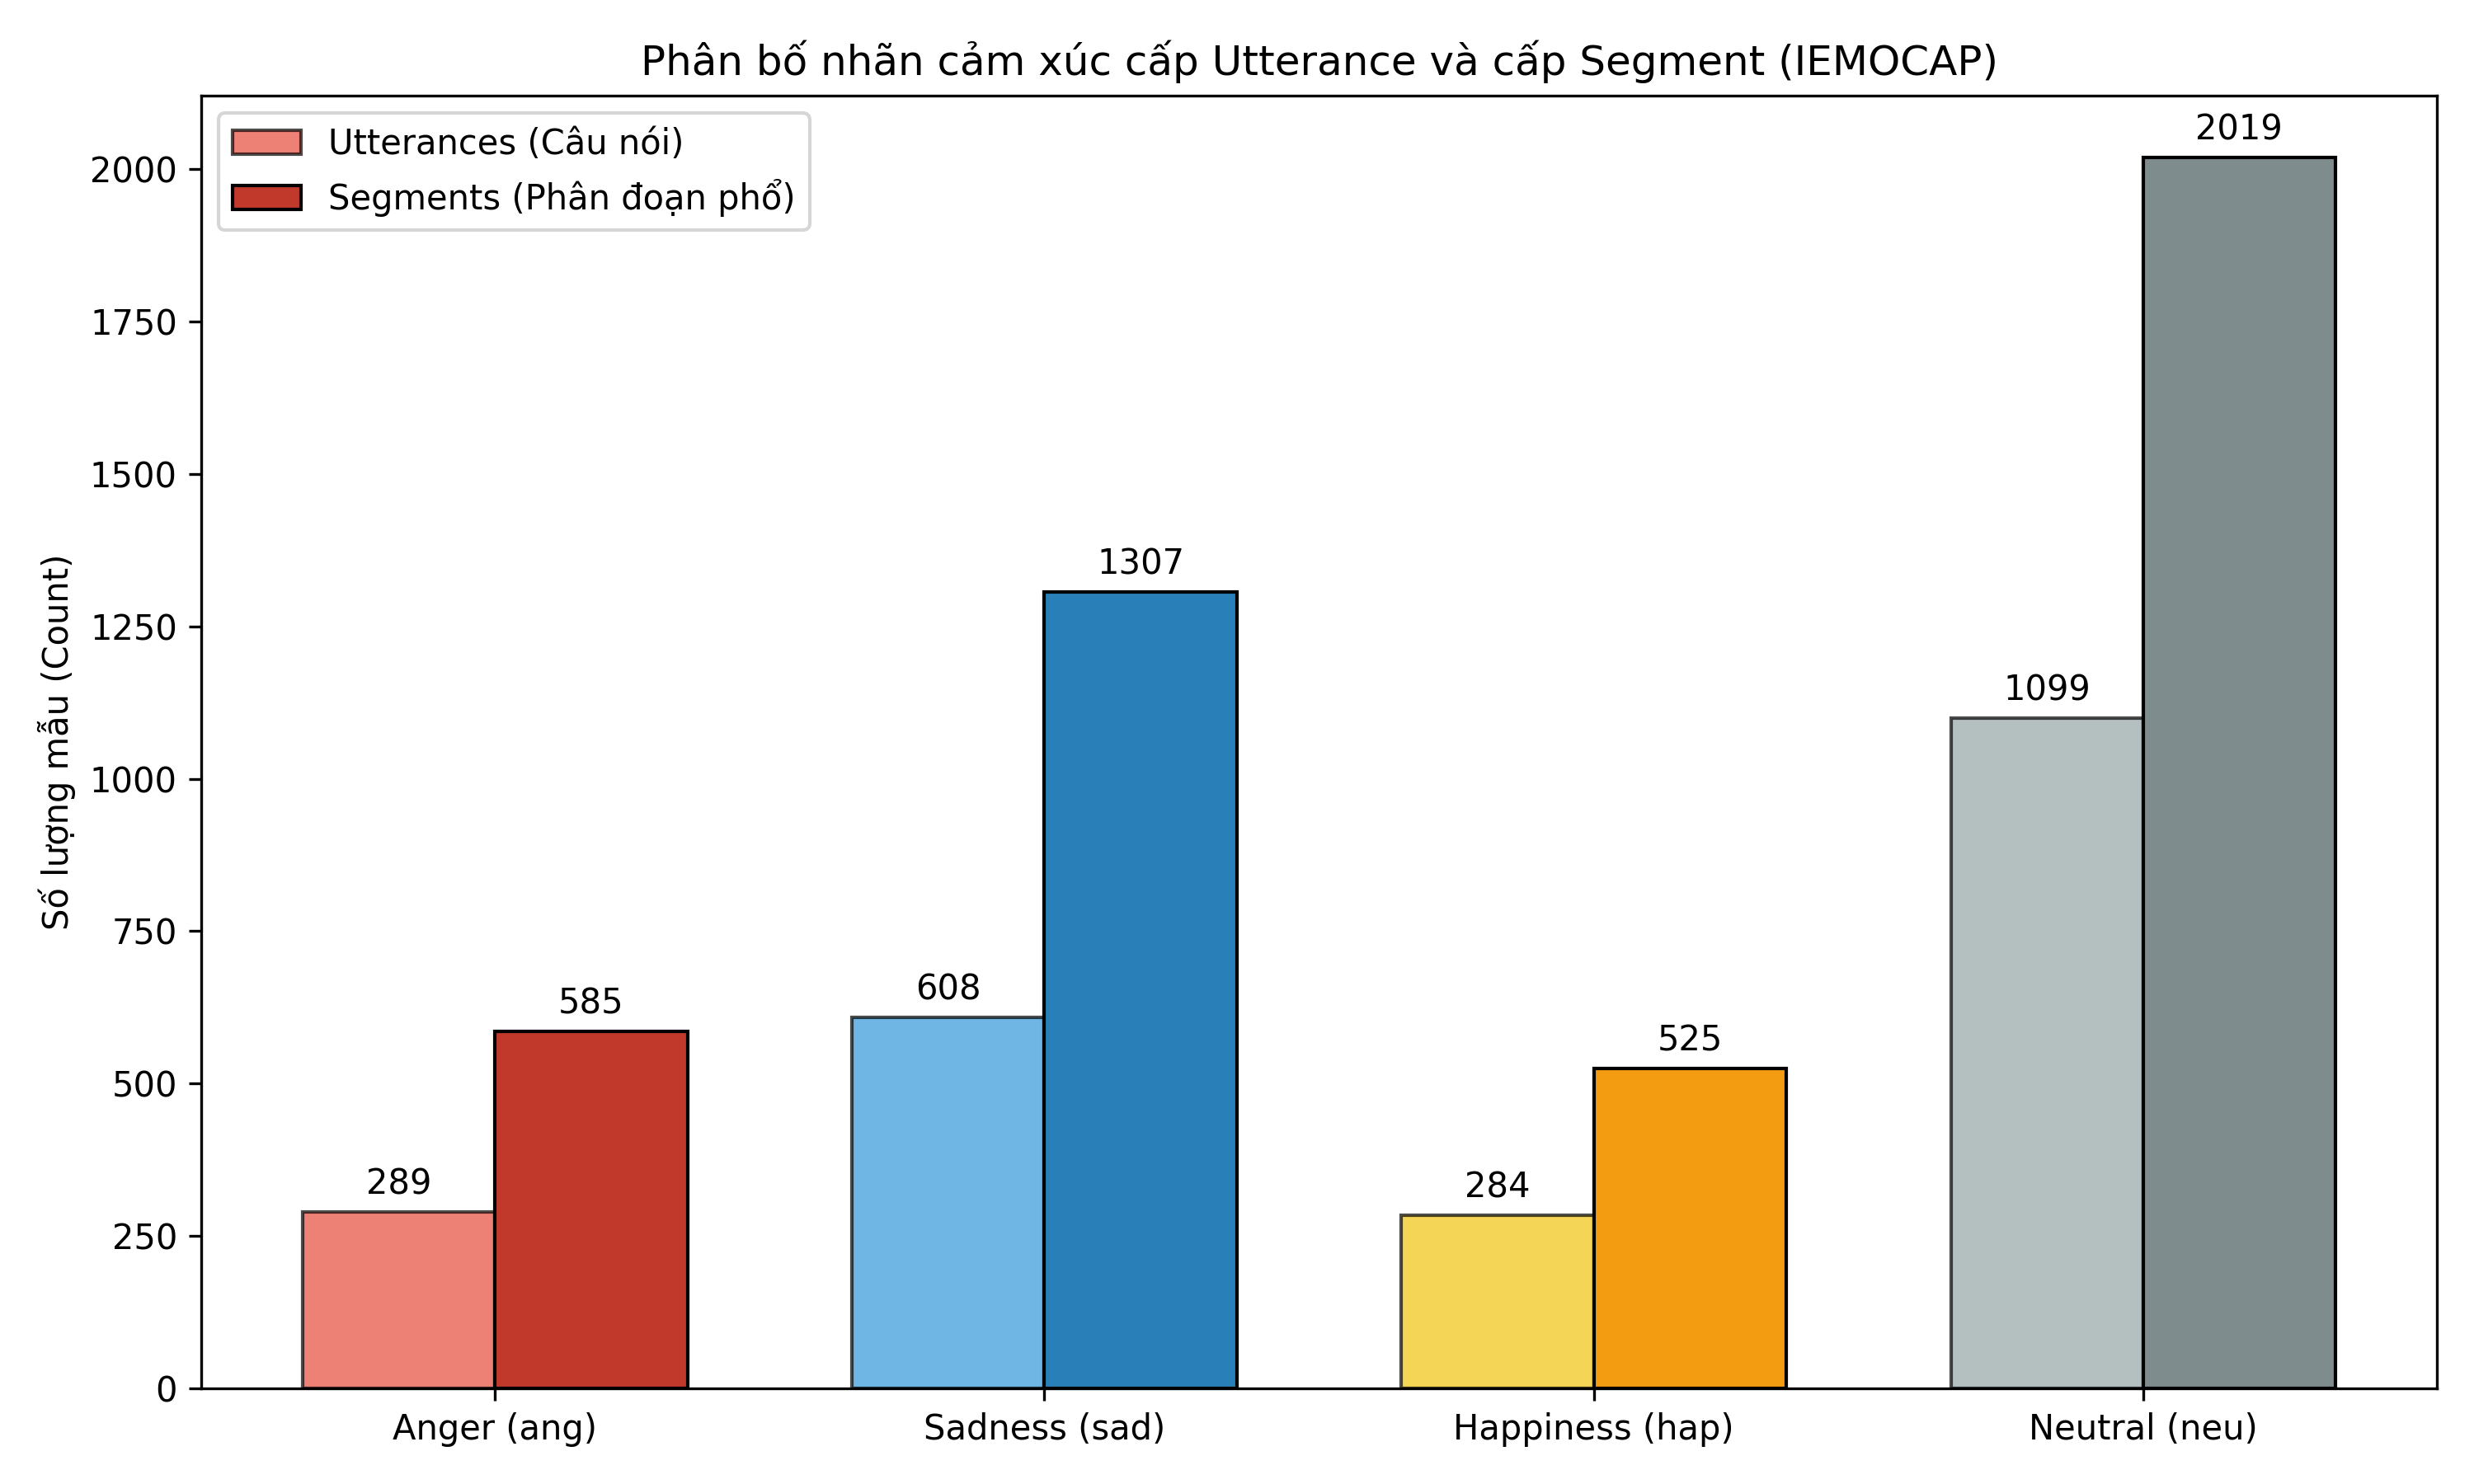
\includegraphics[width=0.75\textwidth]{data_distribution.png}
    \caption{Biểu đồ phân bổ mẫu theo nhãn cảm xúc và theo speaker}
    \label{fig:data_distribution}
\end{figure}

\begin{figure}[H]
    \centering
    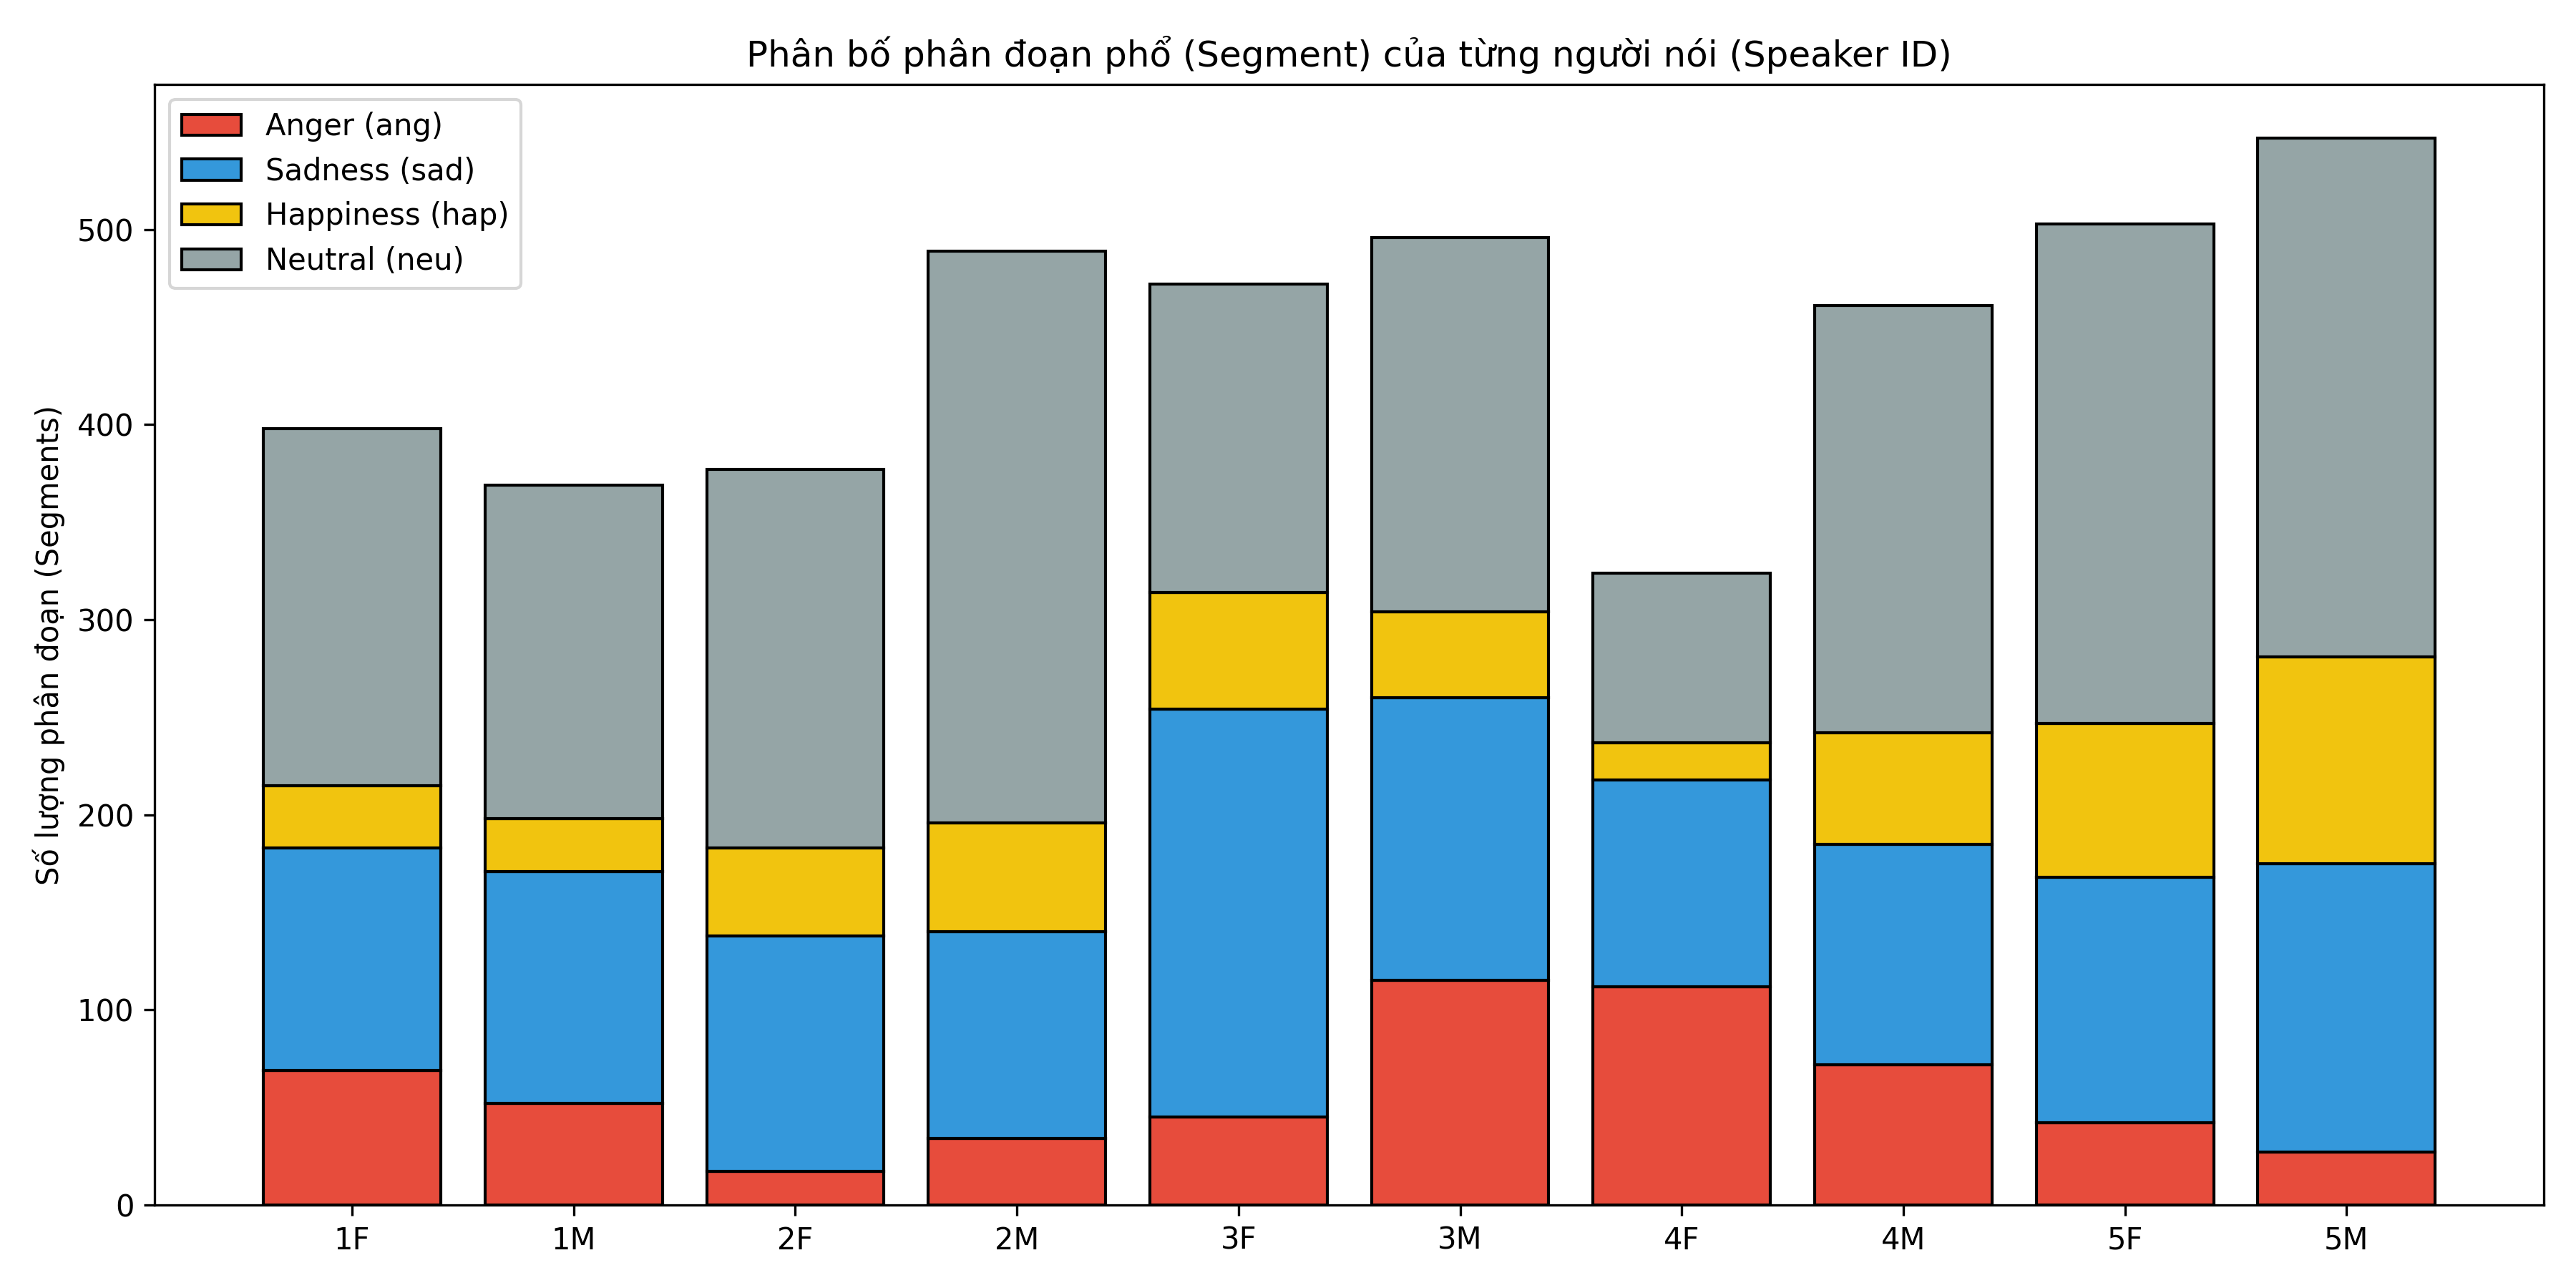
\includegraphics[width=0.75\textwidth]{speaker_distribution.png}
    \caption{Phân bổ mẫu theo từng speaker trong 5 Session}
    \label{fig:speaker_distribution}
\end{figure}

Sự chênh lệch lớn giữa lớp đa số (Neutral: 48,2\%) và lớp thiểu số nhất (Happiness: 12,5\%) lên đến gần 4 lần, đặt ra thách thức lớn về sự mất cân bằng dữ liệu đối với mô hình phân loại. Phân bổ mẫu cụ thể theo từng diễn viên và theo từng session được trực quan hóa lần lượt trong Hình~\ref{fig:data_distribution} và Hình~\ref{fig:speaker_distribution}.


\section{Quy trình tiền xử lý dữ liệu}
\label{sec:preprocessing}

\subsection{Bước 1: Trích xuất đặc trưng Log-Spectrogram}

Quy trình trích xuất đặc trưng được thực hiện thông qua module \path{features_extraction/} sử dụng thư viện \texttt{librosa} \cite{mcfee2015} theo các bước tuần tự bao gồm: resampling tín hiệu về tần số lấy mẫu chuẩn 16 kHz; áp dụng bộ lọc tiền nhấn với hệ số $\alpha = 0.97$; thực hiện phép biến đổi STFT sử dụng cửa sổ Hamming độ dài 40 ms và bước trượt 10 ms với $N_{\text{FFT}} = 800$; thực hiện chuyển đổi biên độ sang thang đo decibel; và cuối cùng là giữ lại 200 băng tần số thấp nhất để tạo thành ma trận đặc trưng Log-Spectrogram.

\subsection{Bước 2: Phân đoạn (Segmentation)}

Do mỗi câu nói có thời lượng khác nhau, ma trận phổ đồ tương ứng sẽ có chiều dài thời gian khác nhau. Để đưa dữ liệu vào huấn luyện mạng CNN một cách hiệu quả, hệ thống tiến hành cắt ma trận phổ đồ thành các phân đoạn độc lập có kích thước cố định $200 \times 300$, tương đương khoảng 3 giây âm thanh. Đối với các câu nói ngắn hơn 300 khung thời gian, việc đệm để đạt chiều dài chuẩn sẽ được thực hiện sau bước chuẩn hóa MinMax về dải $[0.0, 1.0]$ bằng cách đệm thêm giá trị $0.0$ (tương ứng với mức năng lượng tối thiểu $-80\,\text{dB}$ ban đầu). Phương pháp này giúp tránh hiện tượng đệm trực tiếp giá trị $0$ trên thang decibel vốn biểu thị mức năng lượng âm học cực đại ($0\,\text{dB}$). Phân bổ mẫu ở cấp phân đoạn được tổng hợp chi tiết trong Bảng~\ref{tab:segment_distribution}.

\begin{table}[H]
\centering
\caption{Thống kê phân bổ mẫu theo nhãn cảm xúc (cấp phân đoạn)}
\label{tab:segment_distribution}
\begin{tabular}{lcc}
\toprule
\textbf{Nhãn cảm xúc} & \textbf{Số phân đoạn} & \textbf{Tỉ lệ (\%)} \\
\midrule
Neutral & 2.019 & 45,5 \\
Sadness & 1.307 & 29,5 \\
Anger & 585 & 13,2 \\
Happiness & 525 & 11,8 \\
\midrule
\textbf{Tổng cộng} & \textbf{4.436} & \textbf{100,0} \\
\bottomrule
\end{tabular}
\end{table}

\subsection{Bước 3: Chuẩn hóa và định dạng ảnh đầu vào}

Quy trình chuẩn hóa và định dạng ảnh đầu vào được thiết lập qua ba bước chính. Trước tiên, hệ thống áp dụng chuẩn hóa MinMax trên tập Train để chuyển đổi dải giá trị decibel của phổ đồ từ $[-80\,\text{dB}, 0\,\text{dB}]$ về khoảng $[0.0, 1.0]$, cùng bộ scaler này sau đó được áp dụng đồng bộ cho tập Validation và tập Test. Sau đó, phần đệm thời gian cho các câu ngắn sẽ được điền giá trị $0.0$ để đưa về kích thước chuẩn $200 \times 300$. Tiếp theo, đặc trưng được chuyển đổi sang dạng Pseudo-RGB bằng cách lật ngược trục tần số và nhân bản kênh đơn thành 3 kênh giống nhau để tạo thành tensor kích thước $(3 \times 200 \times 300)$. Cuối cùng, tensor được resize về kích thước chuẩn $256 \times 256$ pixels và thực hiện chuẩn hóa Z-Score theo các giá trị trung bình và độ lệch chuẩn của bộ dữ liệu ImageNet. 

Cần lưu ý rằng việc nhân bản kênh đơn thành 3 kênh để áp dụng mô hình pre-trained từ ImageNet tồn tại một hạn chế về mặt lý thuyết (domain mismatch). ImageNet chứa các hình ảnh tự nhiên có tính chất bất biến tịnh tiến không gian (spatial translation invariance), trong khi phổ đồ âm thanh là biểu diễn thời gian-tần số (time-frequency) mà việc dịch chuyển theo trục dọc làm thay đổi cao độ (pitch) và thay đổi ngữ nghĩa. Thêm vào đó, việc nhân bản 3 kênh giống hệt nhau khiến các bộ lọc tích chập ở lớp đầu tiên nhận thông tin thừa. Tuy nhiên, phương pháp này được chấp nhận rộng rãi như một kỹ thuật kỹ nghệ thực hành thông dụng, giúp tận dụng các bộ lọc thô đã được tối ưu trước (như phát hiện các đường biên, vân bề mặt và kết cấu) từ ImageNet để học các họa âm (harmonics) và điểm chuyển tiếp trên phổ đồ nhanh hơn.


\section{Phân chia dữ liệu Speaker-Independent}
\label{sec:speaker_independent}

Để đảm bảo mô hình có khả năng tổng quát hóa tốt trên giọng nói của người lạ (người nói không xuất hiện trong tập huấn luyện), dữ liệu được phân chia theo nguyên tắc Speaker-Independent nghiêm ngặt như được mô tả trong Bảng~\ref{tab:speaker_split}.

\begin{table}[H]
\centering
\caption{Phân chia dữ liệu theo Speaker-Independent}
\label{tab:speaker_split}
\begin{tabular}{lll}
\toprule
\textbf{Tập dữ liệu} & \textbf{Số speaker} & \textbf{Mô tả} \\
\midrule
Train & 8 speakers (4 sessions) & Huấn luyện mô hình \\
Validation & 1 speaker & Chọn mô hình tốt nhất \\
Test & 1 speaker & Đánh giá cuối cùng \\
\bottomrule
\end{tabular}
\end{table}

Ví dụ, với cấu hình mặc định (val=1F, test=1M), 8 speakers từ Session 2--5 được sử dụng làm tập huấn luyện, diễn viên nữ của Session 1 (1F) làm validation, và diễn viên nam của Session 1 (1M) làm tập test. Để ngăn chặn hoàn tượng rò rỉ dữ liệu (data leakage) giữa các tập dữ liệu, quy trình phân chia theo danh tính người nói (Speaker ID) được thực hiện một cách nghiêm ngặt trên cấp độ câu nói (Utterance) trước khi cắt phân đoạn.

Tuy nhiên, thiết lập phân chia này vẫn tồn tại một hạn chế âm học thực tế. Do diễn viên validation (nữ) và diễn viên test (nam) trong mỗi cấu hình thuộc về cùng một Session (ví dụ Session 1), hai người này nói chuyện trực tiếp trong cùng một phòng thu với cùng hệ thống microphone và nhiễu nền tĩnh. Do đó, mô hình có thể vô tình khai thác các đặc tính tĩnh của kênh truyền (channel characteristics) hoặc nhiễu phòng chung từ tập validation để cải thiện dự đoán trên tập test. Đây là một dạng rò rỉ âm học môi trường nhẹ (acoustic environment leakage) làm giảm phần nào tính độc lập môi trường tuyệt đối của hệ thống kiểm thử, và sẽ được khắc phục bằng phương pháp Leave-One-Session-Out (LOSO) thực thụ trong các nghiên cứu tiếp theo. Danh sách cụ thể của 10 diễn viên trong bộ dữ liệu được liệt kê trong Bảng~\ref{tab:speakers}.

\begin{table}[H]
\centering
\caption{Danh sách 10 Speaker trong IEMOCAP}
\label{tab:speakers}
\begin{tabular}{cccc}
\toprule
\textbf{Session} & \textbf{Speaker ID} & \textbf{Giới tính} & \textbf{Ký hiệu} \\
\midrule
Session 1 & Speaker 1 & Nữ / Nam & 1F / 1M \\
Session 2 & Speaker 2 & Nữ / Nam & 2F / 2M \\
Session 3 & Speaker 3 & Nữ / Nam & 3F / 3M \\
Session 4 & Speaker 4 & Nữ / Nam & 4F / 4M \\
Session 5 & Speaker 5 & Nữ / Nam & 5F / 5M \\
\bottomrule
\end{tabular}
\end{table}


\section{Kiến trúc mô hình}
\label{sec:model_architecture}

Tất cả các mô hình CNN được xây dựng trong đồ án đều kế thừa một giao diện đồng nhất để dễ dàng tích hợp và đánh giá. Cụ thể, các mô hình nhận đầu vào là tensor kích thước $(N, 3, 256, 256)$ đại diện cho batch ảnh phổ đồ Pseudo-RGB đã chuẩn hóa và trả về đầu ra là các logits kích thước $(N, 4)$ tương ứng với 4 lớp cảm xúc. Các mô hình được khởi tạo sử dụng trọng số pre-trained từ ImageNet để chuyển giao tri thức và chỉ thực hiện sửa đổi lớp phân loại kết nối đầy đủ cuối cùng phù hợp với số lượng lớp cảm xúc của bài toán. Chi tiết tổng hợp về số lượng tham số và đặc điểm của các mô hình được trình bày trong Bảng~\ref{tab:model_summary}.

\begin{table}[H]
\centering
\caption{Tổng hợp các kiến trúc mô hình}
\label{tab:model_summary}
\begin{tabular}{lllr}
\toprule
\textbf{Mô hình} & \textbf{Đặc điểm chính} & \textbf{Lớp phân loại} & \textbf{Tham số} \\
\midrule
AlexNet & 5 Conv + 3 FC & FC(4096, 4) & 57,02M \\
AlexNet GAP & 5 Conv + GAP & Conv $1\times1$ + AvgPool & 2,47M \\
ResNet-18 & Skip Connection & FC(512, 4) & 11,18M \\
DenseNet-121 & Dense Block & FC(1024, 4) & 6,96M \\
EfficientNet-B0 & Compound Scaling & FC(1280, 4) & 4,01M \\
MobileNet-V2 & Depthwise Conv & FC(1280, 4) & 2,23M \\
\bottomrule
\end{tabular}
\end{table}


\section{Quy trình huấn luyện}
\label{sec:training_procedure}

\subsection{Cấu hình huấn luyện}

Bảng~\ref{tab:training_config} trình bày cấu hình siêu tham số huấn luyện được thiết lập đồng nhất cho tất cả các mô hình trong các lượt thực nghiệm nhằm đảm bảo tính công bằng của các so sánh.

\begin{table}[H]
\centering
\caption{Cấu hình huấn luyện chung}
\label{tab:training_config}
\begin{tabular}{ll}
\toprule
\textbf{Tham số} & \textbf{Giá trị} \\
\midrule
Optimizer & AdamW \\
Learning rate & $10^{-4}$ \\
Batch size & 64 \\
Epochs & 60 \\
Random seed & 100 \\
GPU & NVIDIA RTX 3060 (12GB) \\
Framework & PyTorch \\
\bottomrule
\end{tabular}
\end{table}

\subsection{Chiến lược chọn mô hình tốt nhất}

Sau mỗi epoch huấn luyện, mô hình được đánh giá trực tiếp trên tập Validation. Để giải quyết triệt để vấn đề mất cân bằng dữ liệu, hệ thống tự động theo dõi và lưu lại cấu hình trọng số tương ứng với kết quả Unweighted Accuracy (UA) đạt giá trị cao nhất trên tập Validation thay vì dựa vào chỉ số Weighted Accuracy nhằm tránh việc mô hình bị thiên lệch vào lớp đa số. Khi kết thúc quá trình huấn luyện, cấu hình trọng số tối ưu này sẽ được nạp lại để tiến hành đánh giá khách quan trên tập kiểm thử độc lập.

\subsection{Chiến lược đánh giá cấp câu nói (Utterance-level)}

Do mỗi câu nói có thể được phân cắt thành nhiều phân đoạn khác nhau, việc dự đoán nhãn cảm xúc ở cấp câu nói được thực hiện bằng cách tính trung bình hóa xác suất dự đoán (log-softmax) của toàn bộ các phân đoạn thuộc cùng một câu nói, sau đó áp dụng phép lấy cực đại (argmax):
\begin{equation}
    \hat{y}_u = \argmax_c \left( \frac{1}{|\mathcal{S}_u|} \sum_{s \in \mathcal{S}_u} \log P(c | s) \right)
    \label{eq:utt_pred}
\end{equation}
trong đó $\mathcal{S}_u$ là tập hợp tất cả các phân đoạn được cắt ra từ câu nói $u$.


\section{Các chỉ số đánh giá}
\label{sec:metrics}

Hiệu năng của mô hình được đánh giá toàn diện qua ba chỉ số chính. Đầu tiên là Weighted Accuracy (WA) đo lường tỉ lệ dự đoán chính xác trên tổng số mẫu thực tế. Chỉ số thứ hai là Unweighted Accuracy (UA) được tính bằng trung bình cộng độ chính xác của từng lớp cảm xúc độc lập không phụ thuộc vào số lượng mẫu của mỗi lớp, phản ánh chính xác khả năng phân loại đồng đều trên dữ liệu mất cân bằng. Cuối cùng, ma trận nhầm lẫn (Confusion Matrix) kích thước $4 \times 4$ được sử dụng để trực quan hóa số lượng mẫu phân loại đúng và sai lệch giữa các cặp lớp cảm xúc, giúp xác định chi tiết điểm yếu của từng mô hình.


% ====== CHƯƠNG 4: THỰC NGHIỆM VÀ KẾT QUẢ ======
% ============================================================
% CHƯƠNG 4: THỰC NGHIỆM VÀ KẾT QUẢ
% ============================================================
\chapter{Thực nghiệm và kết quả}
\label{chap:experiments}

\section{Cấu hình thực nghiệm}
\label{sec:experiment_setup}

Toàn bộ thực nghiệm được thực hiện trên cùng một cấu hình phần cứng và phần mềm:

\begin{table}[H]
\centering
\caption{Cấu hình môi trường thực nghiệm}
\label{tab:env_config}
\begin{tabular}{ll}
\toprule
\textbf{Thành phần} & \textbf{Chi tiết} \\
\midrule
GPU & NVIDIA GeForce RTX 3060 (12GB VRAM) \\
Python & 3.10 (Miniforge / Conda) \\
Framework & PyTorch 1.6+ \\
Optimizer & AdamW \\
Learning rate & $10^{-4}$ \\
Batch size & 64 \\
Số epochs & 60 \\
Random seed & 100 \\
Phân chia dữ liệu & Speaker-Independent (val=1F, test=1M) \\
\bottomrule
\end{tabular}
\end{table}

Hệ thống tự động lưu các artifact sau mỗi lượt huấn luyện bao gồm trọng số mô hình tốt nhất dạng tệp tin \texttt{.pth}, biểu đồ thể hiện các đường cong học tập (learning curves) lưu dưới dạng ảnh \texttt{*\_curves.png}, và ma trận nhầm lẫn (confusion matrix) dạng heatmap lưu dưới dạng ảnh \texttt{*\_conf.png}.


\section{Kết quả thực nghiệm chính}
\label{sec:main_results}

\subsection{Bảng tổng hợp kết quả}

Bảng~\ref{tab:main_results} trình bày kết quả đánh giá trên tập test (Speaker 1M) cho tất cả 6 cấu hình mô hình. 

\begin{table}[H]
\centering
\setlength{\tabcolsep}{4.5pt}
\caption{Kết quả thực nghiệm trên tập test (val=1F, test=1M)}
\label{tab:main_results}
\begin{tabular}{clllrrrr}
\toprule
\textbf{\#} & \textbf{Mô hình} & \textbf{Loss} & \textbf{Aug.} & \textbf{Params} & \textbf{Test Loss} & \textbf{WA (\%)} & \textbf{UA (\%)} \\
\midrule
1 & AlexNet (Baseline) & CE & Không & 57,02M & 1,2138 & 50,73 & 25,00 \\
2 & AlexNet GAP & CE & Không & 2,47M & 0,9859 & 78,54 & 64,89 \\
3 & ResNet-18 & Focal & EMix-S & 11,18M & 0,4541 & 76,10 & 64,37 \\
4 & DenseNet-121 & Focal & EMix-S & 6,96M & 0,2927 & 68,78 & 66,48 \\
5 & \textbf{EfficientNet-B0} $\star$ & \textbf{Focal} & \textbf{EMix-S} & \textbf{4,01M} & \textbf{0,2792} & \textbf{80,98} & \textbf{74,25} \\
6 & MobileNet-V2 & Focal & EMix-S & 2,23M & 0,3549 & 76,59 & 71,15 \\
\bottomrule
\end{tabular}
\end{table}

Trong số các mô hình đánh giá, cấu hình phối hợp EfficientNet-B0 cùng hàm lỗi Focal Loss và kỹ thuật tăng cường dữ liệu EMix-S mang lại hiệu năng tối ưu nhất trên lượt kiểm thử đơn lẻ này, đạt WA=80,98\% và UA=74,25\%. Tuy nhiên, cần nhận thức rằng thiết lập đánh giá trên một lượt chia (Single Fold) này chịu ảnh hưởng lớn bởi độ dễ/khó ngẫu nhiên của đặc trưng người nói kiểm thử (Speaker 1M) và chưa mang ý nghĩa thống kê đầy đủ do mẫu kiểm thử cảm xúc (như Anger và Happiness) rất hạn chế.

Một điểm đáng chú ý khác trong bảng kết quả baseline là khi so sánh hai mô hình dùng Cross Entropy thuần túy và không có tăng cường dữ liệu: phiên bản AlexNet GAP cải tiến (đạt 64,89\% UA) hoạt động tốt hơn đáng kể so với EfficientNet-B0 cơ sở (chỉ đạt 58,46\% UA, xem Mục~\ref{sec:ablation}). Điều này cho thấy với một bài toán có lượng dữ liệu nhỏ như SER, các mô hình học sâu hiện đại và phức tạp như EfficientNet-B0 rất dễ rơi vào trạng thái quá khớp (overfitting) nếu không có các kỹ thuật điều hòa hoặc tăng cường dữ liệu đi kèm, trong khi cấu hình tích hợp GAP của AlexNet hoạt động ổn định và bền bỉ hơn.

\subsection{Biểu đồ so sánh tổng hợp}

Các biểu đồ trực quan hóa kết quả so sánh giữa các mô hình được thể hiện từ Hình~\ref{fig:comparison_wa_ua} đến Hình~\ref{fig:summary}. Trong đó, Hình~\ref{fig:comparison_wa_ua} biểu diễn độ chính xác WA và UA của cả 6 cấu hình mô hình; Hình~\ref{fig:comparison_params} thể hiện mối quan hệ và sự cân bằng giữa số lượng tham số huấn luyện (model parameters) và Weighted Accuracy; và Hình~\ref{fig:summary} cung cấp cái nhìn tổng hợp về cả độ chính xác tổng thể và độ chính xác chi tiết theo từng lớp cảm xúc.

\begin{figure}[H]
    \centering
    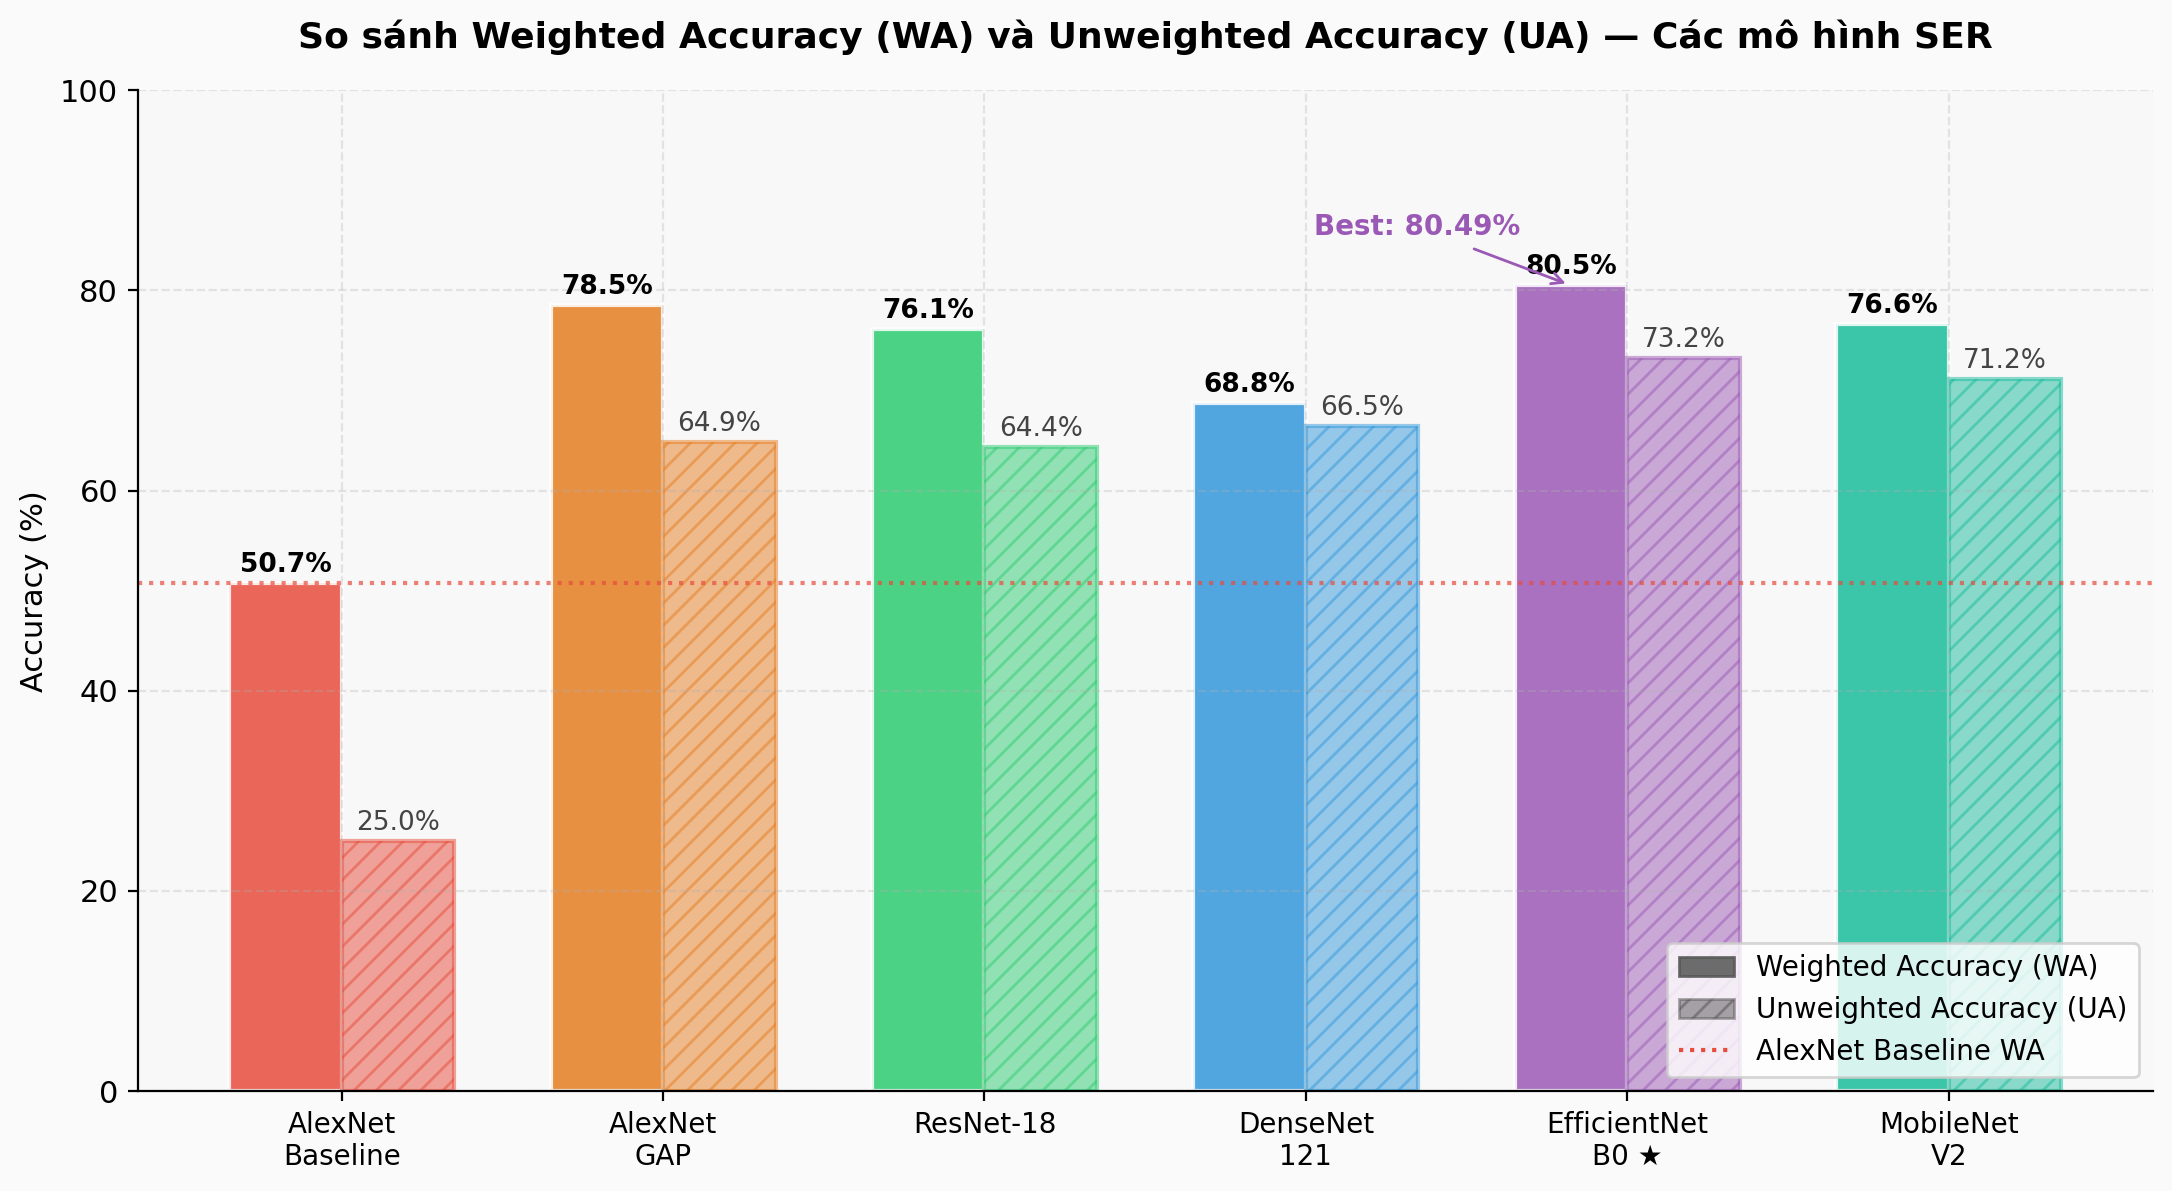
\includegraphics[width=0.85\textwidth]{comparison_wa_ua.png}
    \caption{Biểu đồ so sánh WA và UA giữa các mô hình}
    \label{fig:comparison_wa_ua}
\end{figure}

\begin{figure}[H]
    \centering
    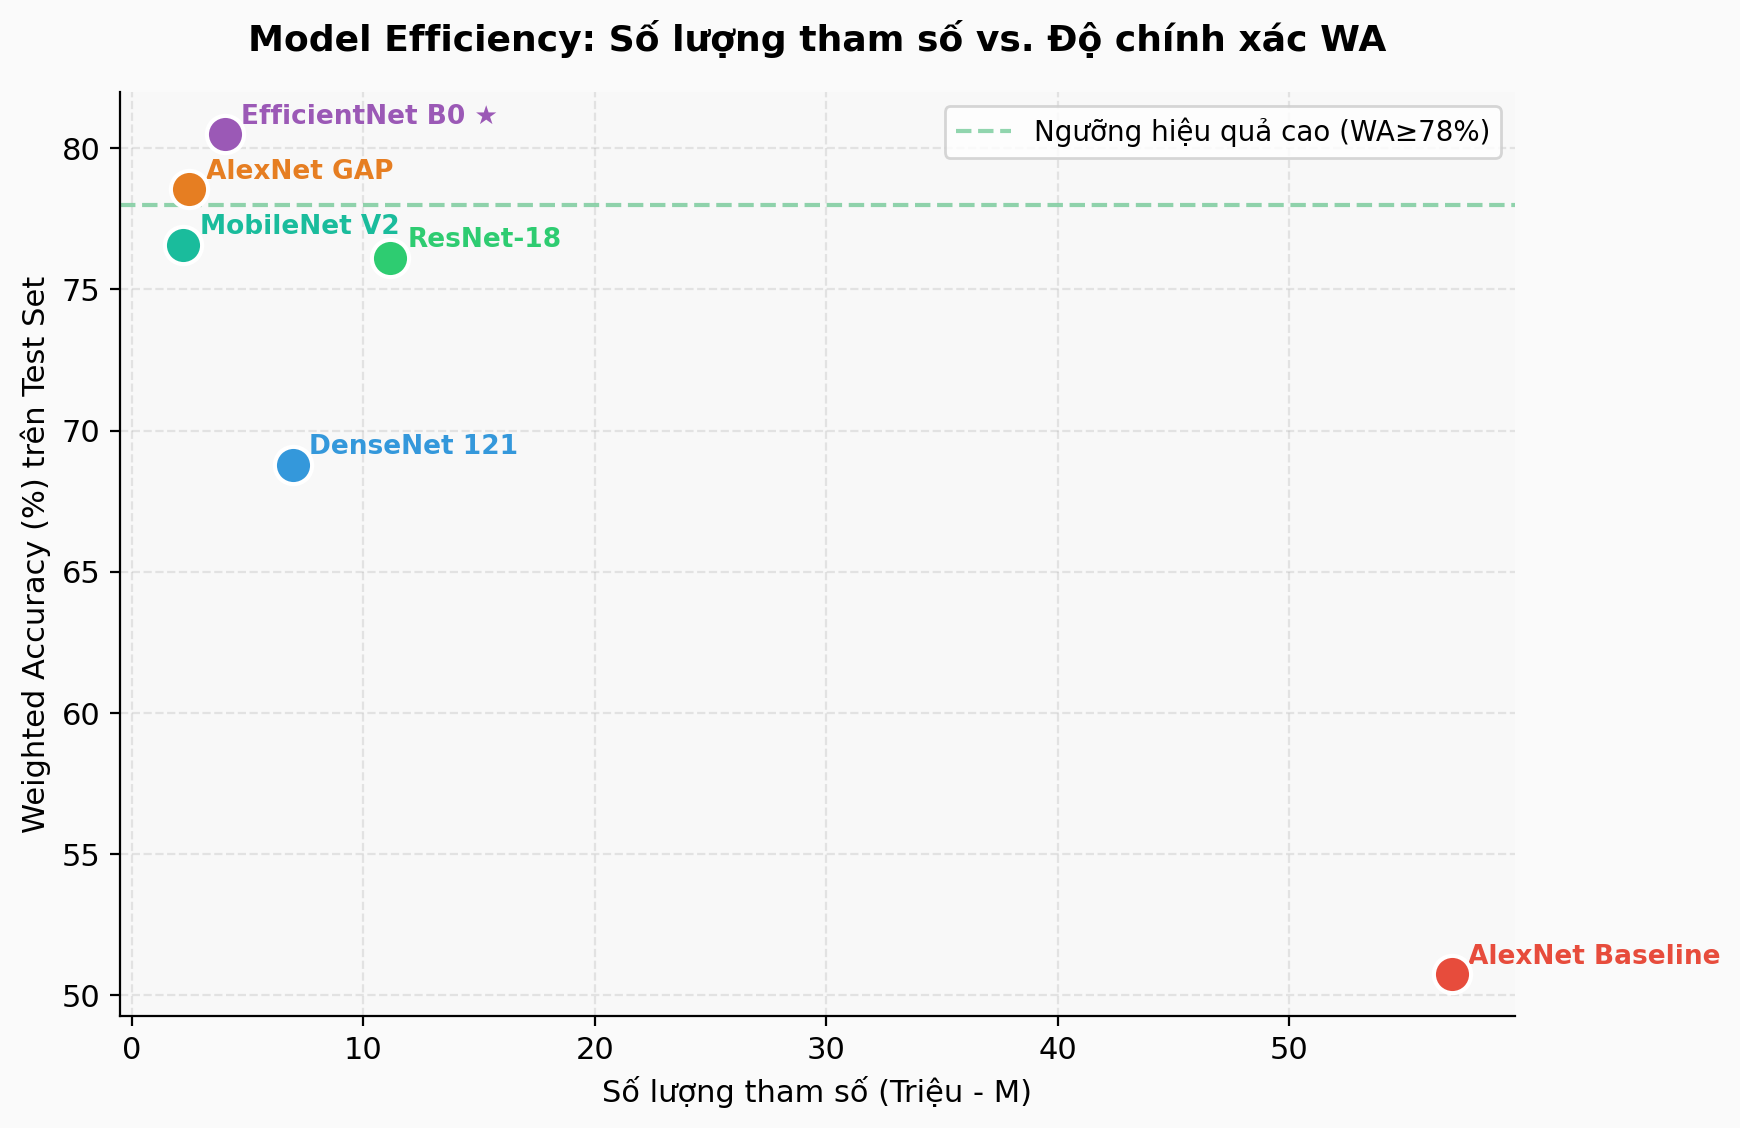
\includegraphics[width=0.85\textwidth]{comparison_params_vs_wa.png}
    \caption{Mối quan hệ giữa số lượng tham số và Weighted Accuracy}
    \label{fig:comparison_params}
\end{figure}

\begin{figure}[H]
    \centering
    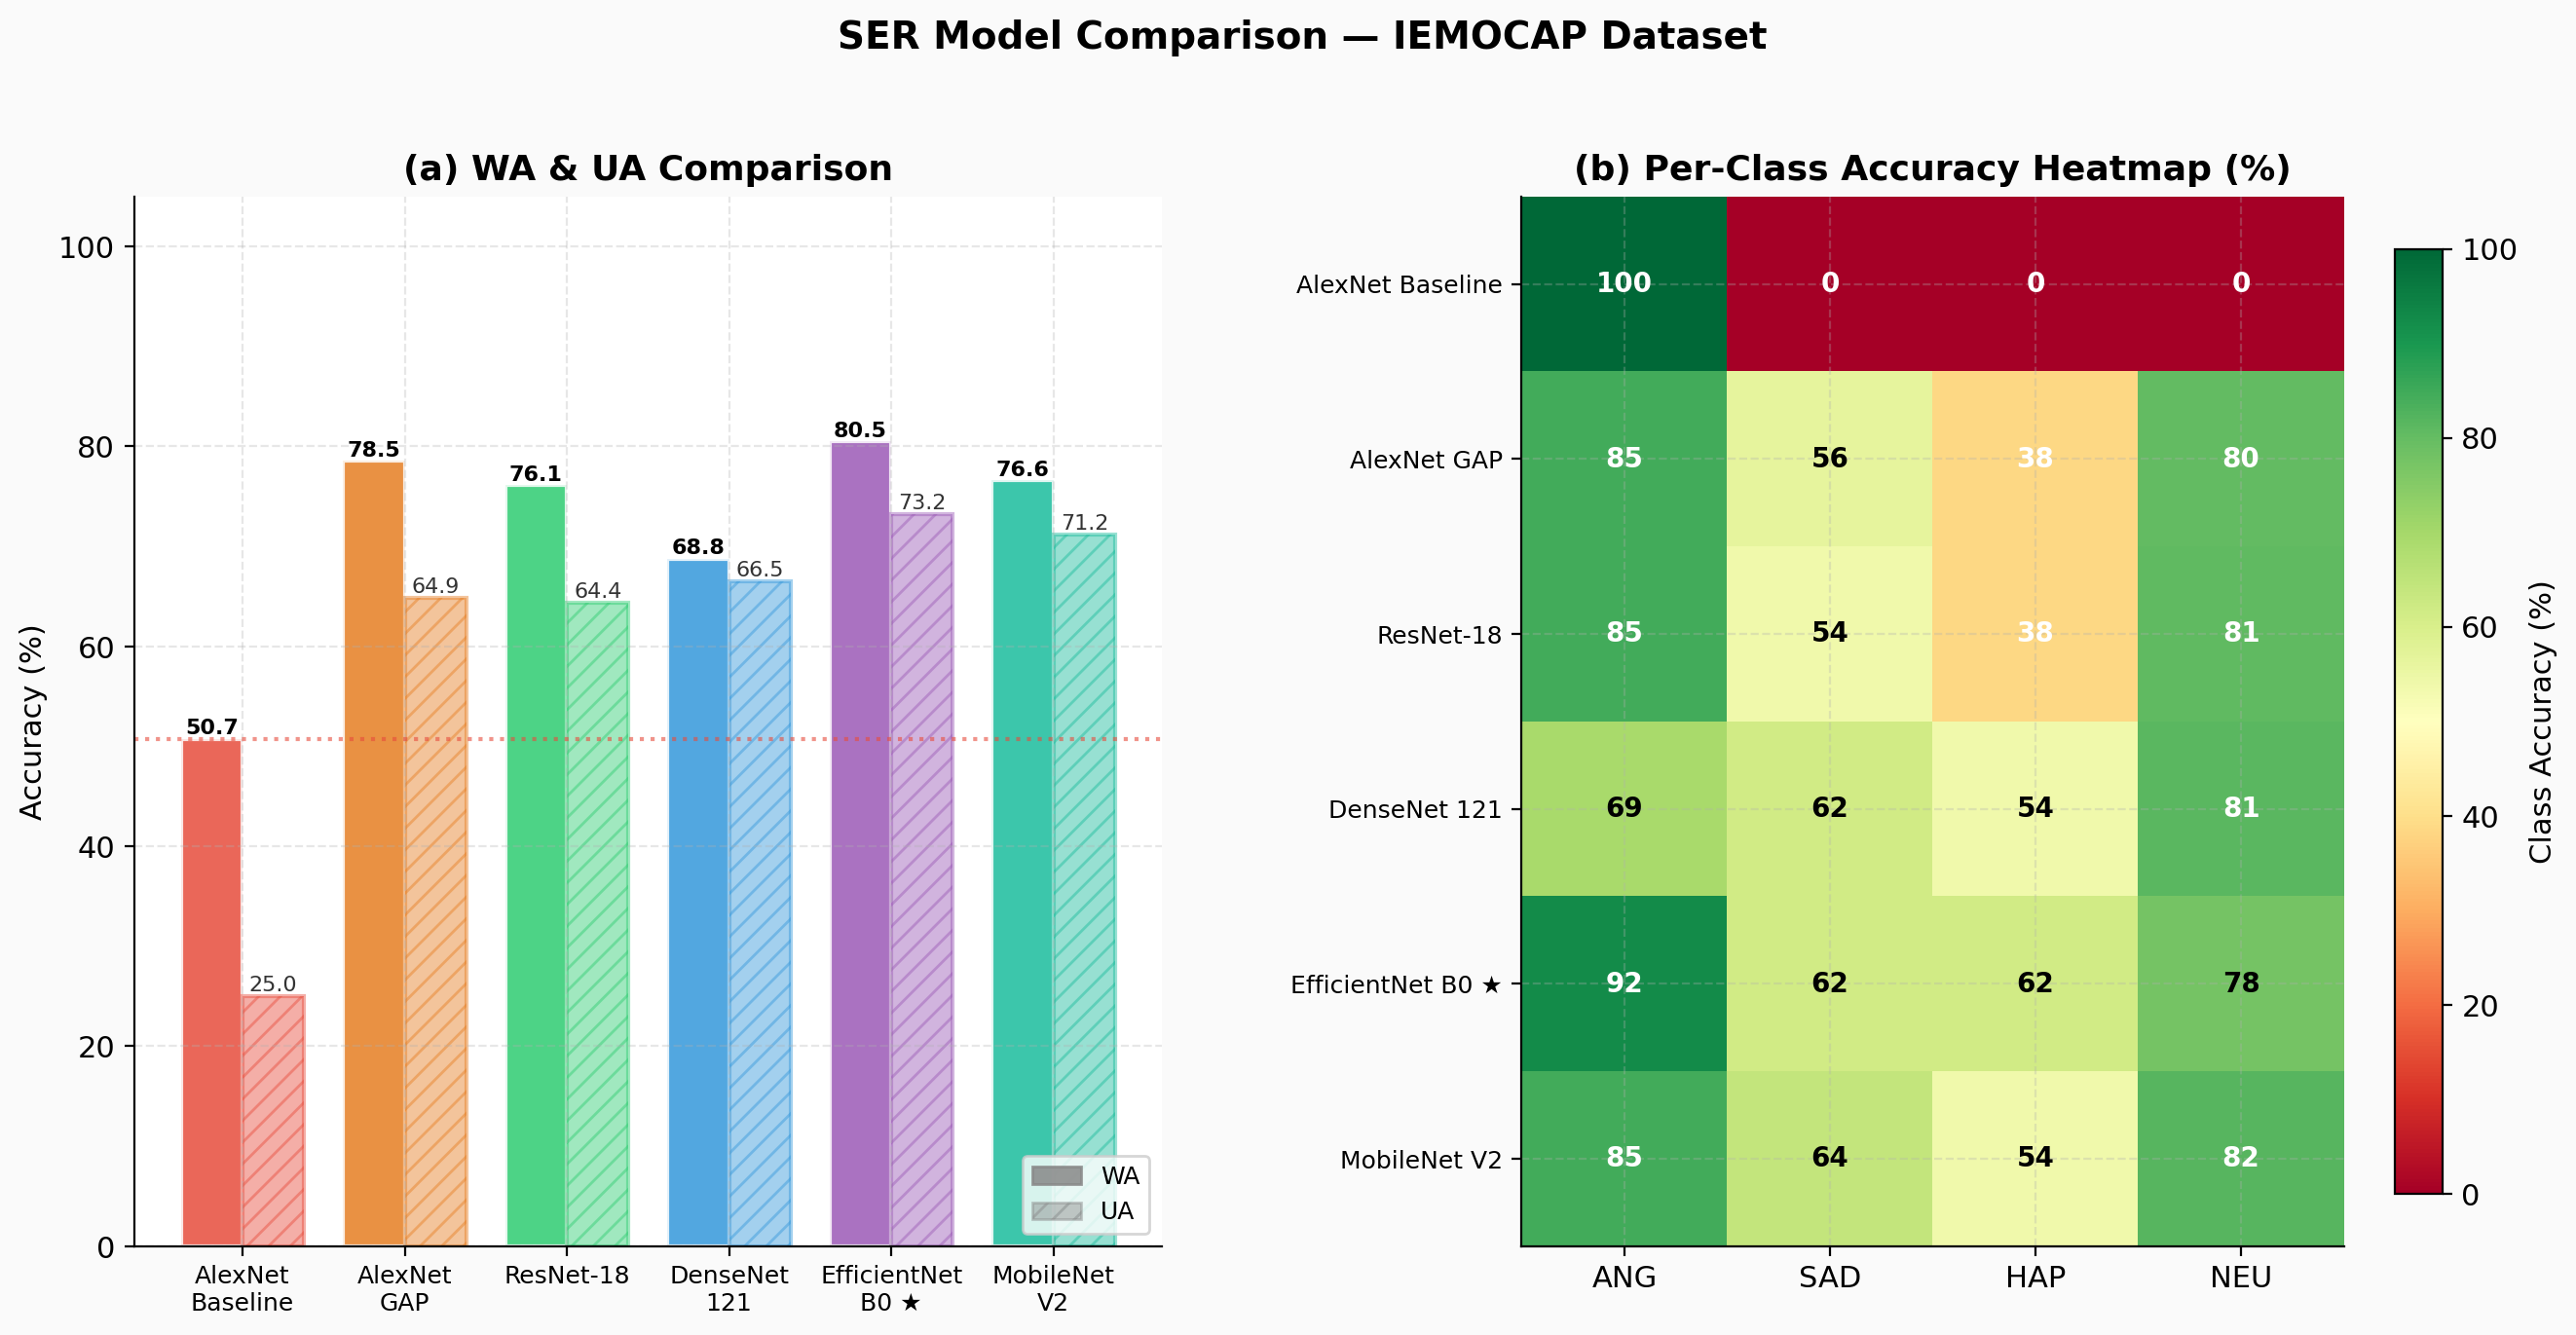
\includegraphics[width=\textwidth]{summary_figure.png}
    \caption{Biểu đồ tổng hợp kết quả thực nghiệm (publication-quality)}
    \label{fig:summary}
\end{figure}


\section{Phân tích chi tiết từng mô hình}
\label{sec:detailed_analysis}

\subsection{AlexNet Baseline (Cross Entropy, Không Augmentation)}

\begin{figure}[H]
    \centering
    \begin{subfigure}[b]{0.55\textwidth}
        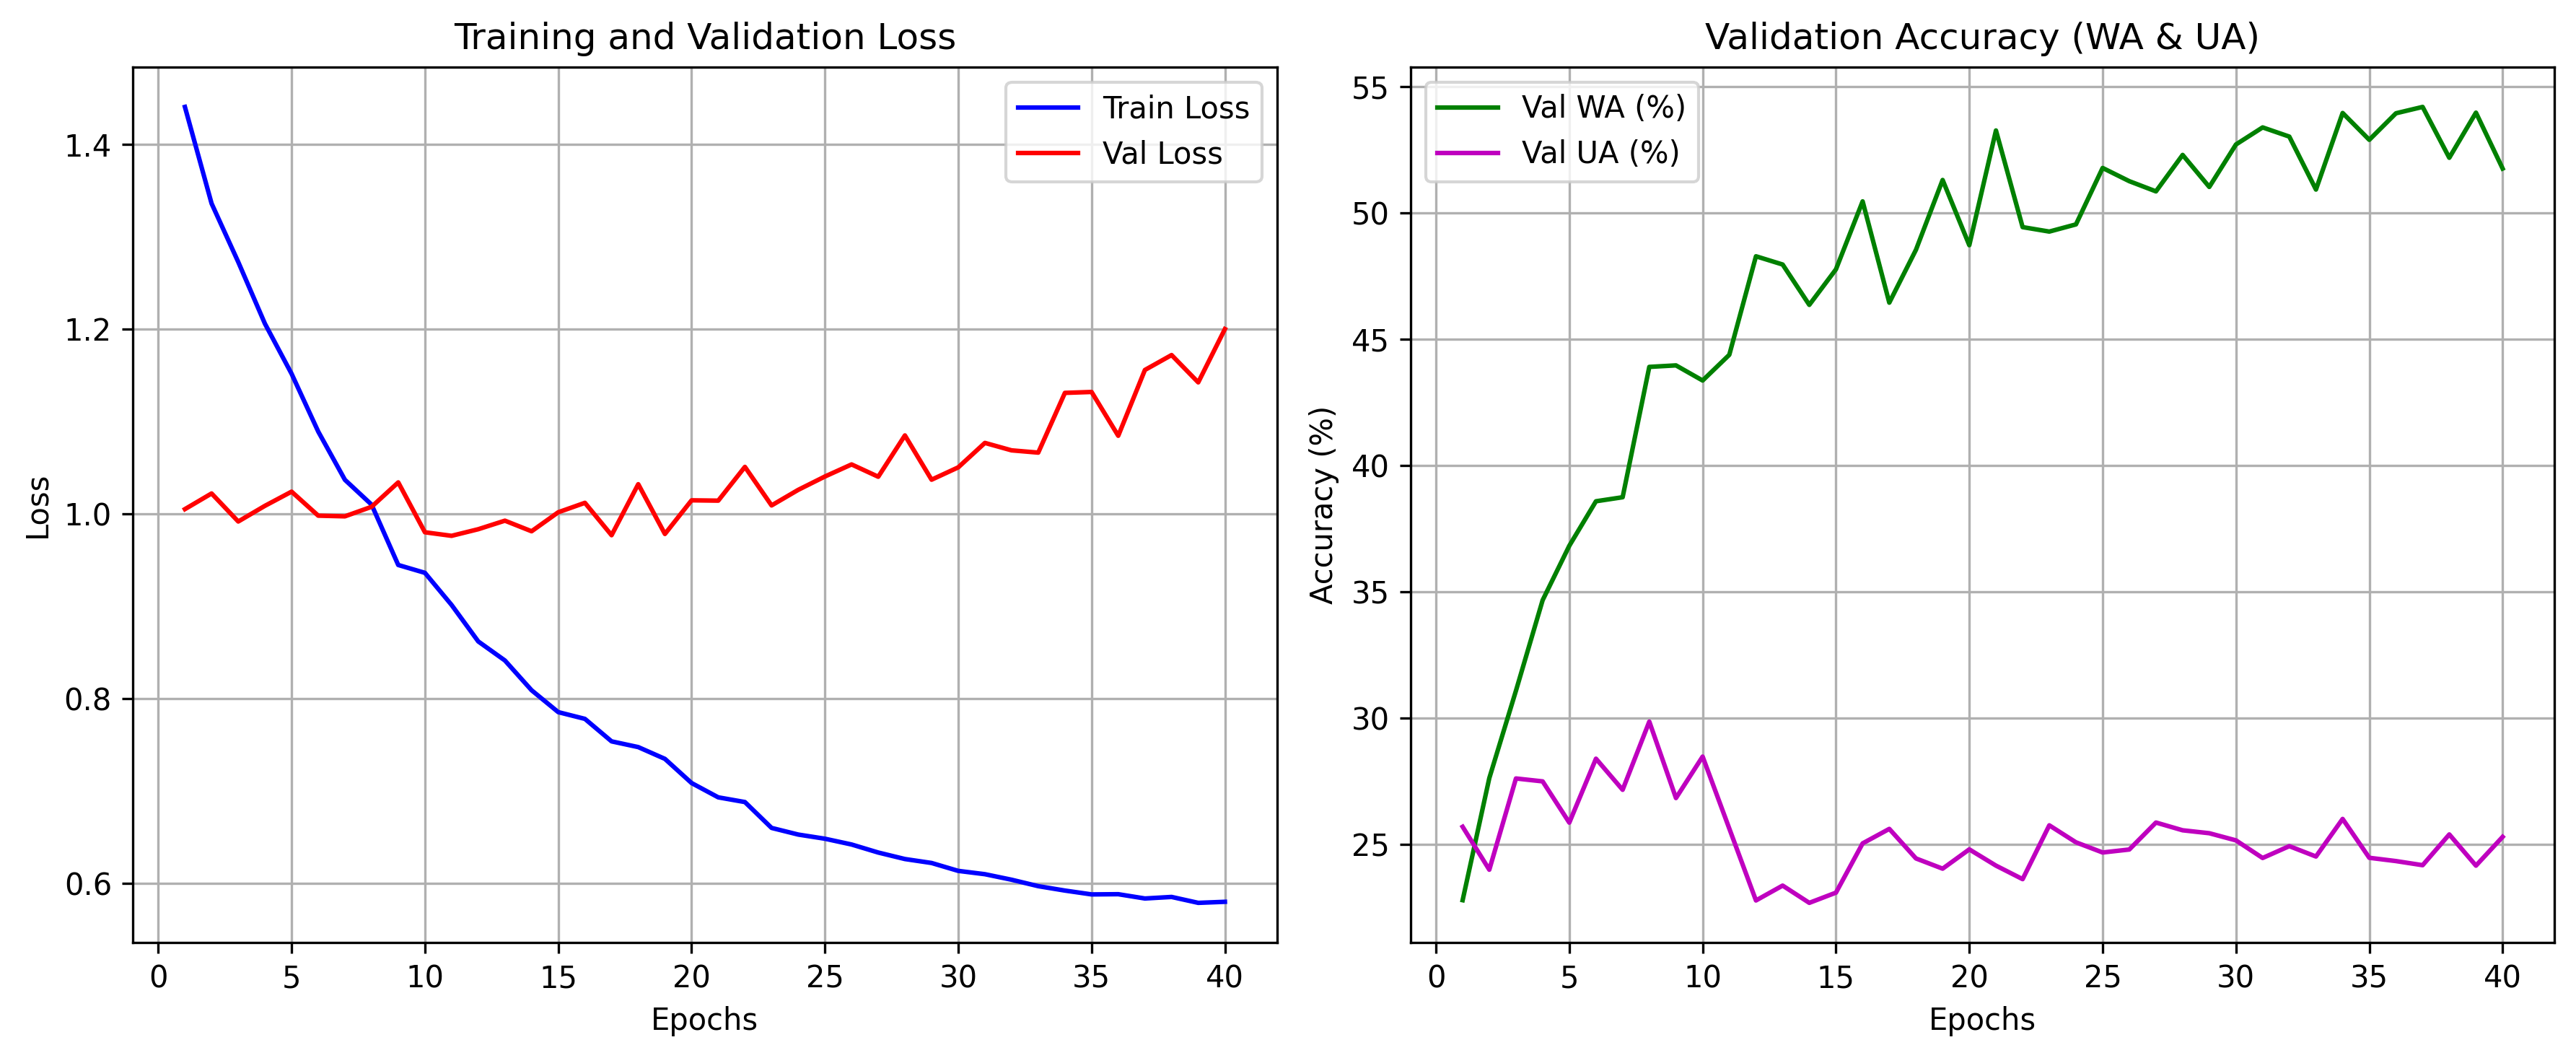
\includegraphics[width=\textwidth]{alexnet_baseline_curves.png}
        \caption{Training/Validation curves}
    \end{subfigure}
    \hfill
    \begin{subfigure}[b]{0.38\textwidth}
        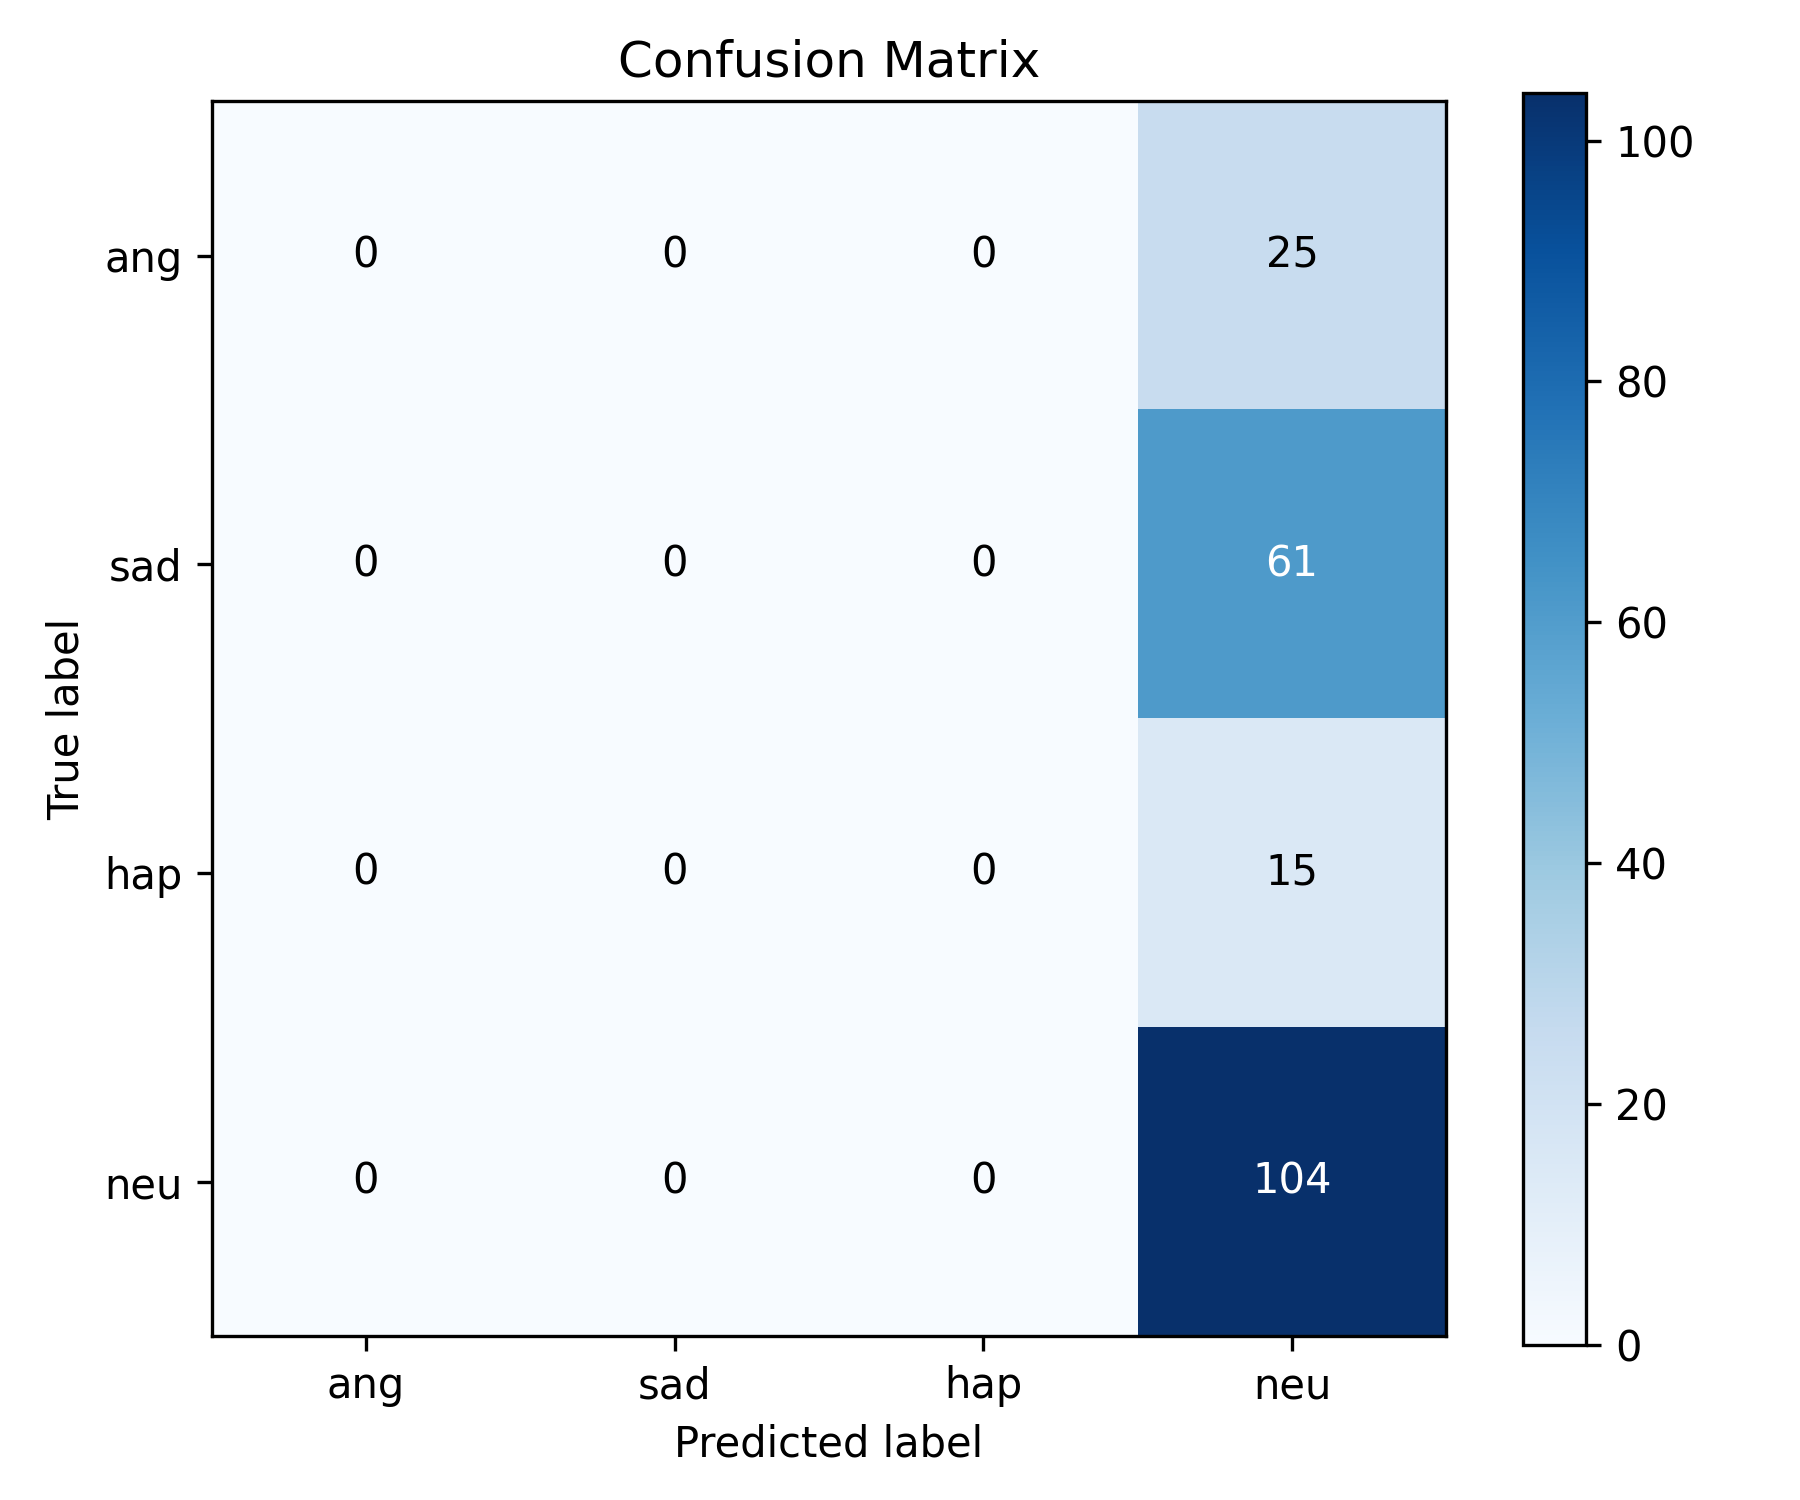
\includegraphics[width=\textwidth]{alexnet_baseline_conf.png}
        \caption{Ma trận nhầm lẫn}
    \end{subfigure}
    \caption{Kết quả AlexNet Baseline: WA=50,73\%, UA=25,00\%}
    \label{fig:alexnet_baseline}
\end{figure}

Kết quả chi tiết được minh họa trong Hình~\ref{fig:alexnet_baseline}, bao gồm đồ thị huấn luyện và ma trận nhầm lẫn của mô hình AlexNet Baseline.

Phân tích kết quả của AlexNet Baseline cho thấy mô hình bị thiên lệch hoàn toàn về phía lớp đa số (majority class bias). Mô hình phân loại toàn bộ các mẫu của tập kiểm thử vào lớp Neutral (lớp chiếm tỷ lệ lớn nhất với 50,73\% tổng số mẫu), dẫn đến độ chính xác của lớp Neutral đạt tuyệt đối 100\% trong khi cả 3 lớp còn lại (Anger, Sadness, Happiness) đều đạt 0\%. Chỉ số UA đạt đúng 25,00\% (tương đương mức dự đoán ngẫu nhiên cho 4 lớp) phản ánh rằng mô hình hoàn toàn không học được các đặc trưng phân biệt ngữ điệu giữa các cảm xúc khác nhau. Nguyên nhân chính dẫn đến hiện tượng này là do kiến trúc AlexNet nguyên bản sở hữu các lớp kết nối đầy đủ (FC) chứa lượng tham số quá lớn (57 triệu tham số) dễ gây ra hiện tượng quá khớp (overfitting) và giảm khả năng tổng quát hóa trên tập dữ liệu nhỏ. Đồng thời, hàm lỗi Cross Entropy truyền thống không thể tự điều chỉnh được ảnh hưởng của sự mất cân bằng dữ liệu cực đoan, thúc đẩy quá trình tối ưu hóa hội tụ về việc dự đoán lớp đa số Neutral nhằm giảm thiểu giá trị loss trung bình trên toàn tập dữ liệu.

\subsection{AlexNet GAP (Cross Entropy)}

\begin{figure}[H]
    \centering
    \begin{subfigure}[b]{0.55\textwidth}
        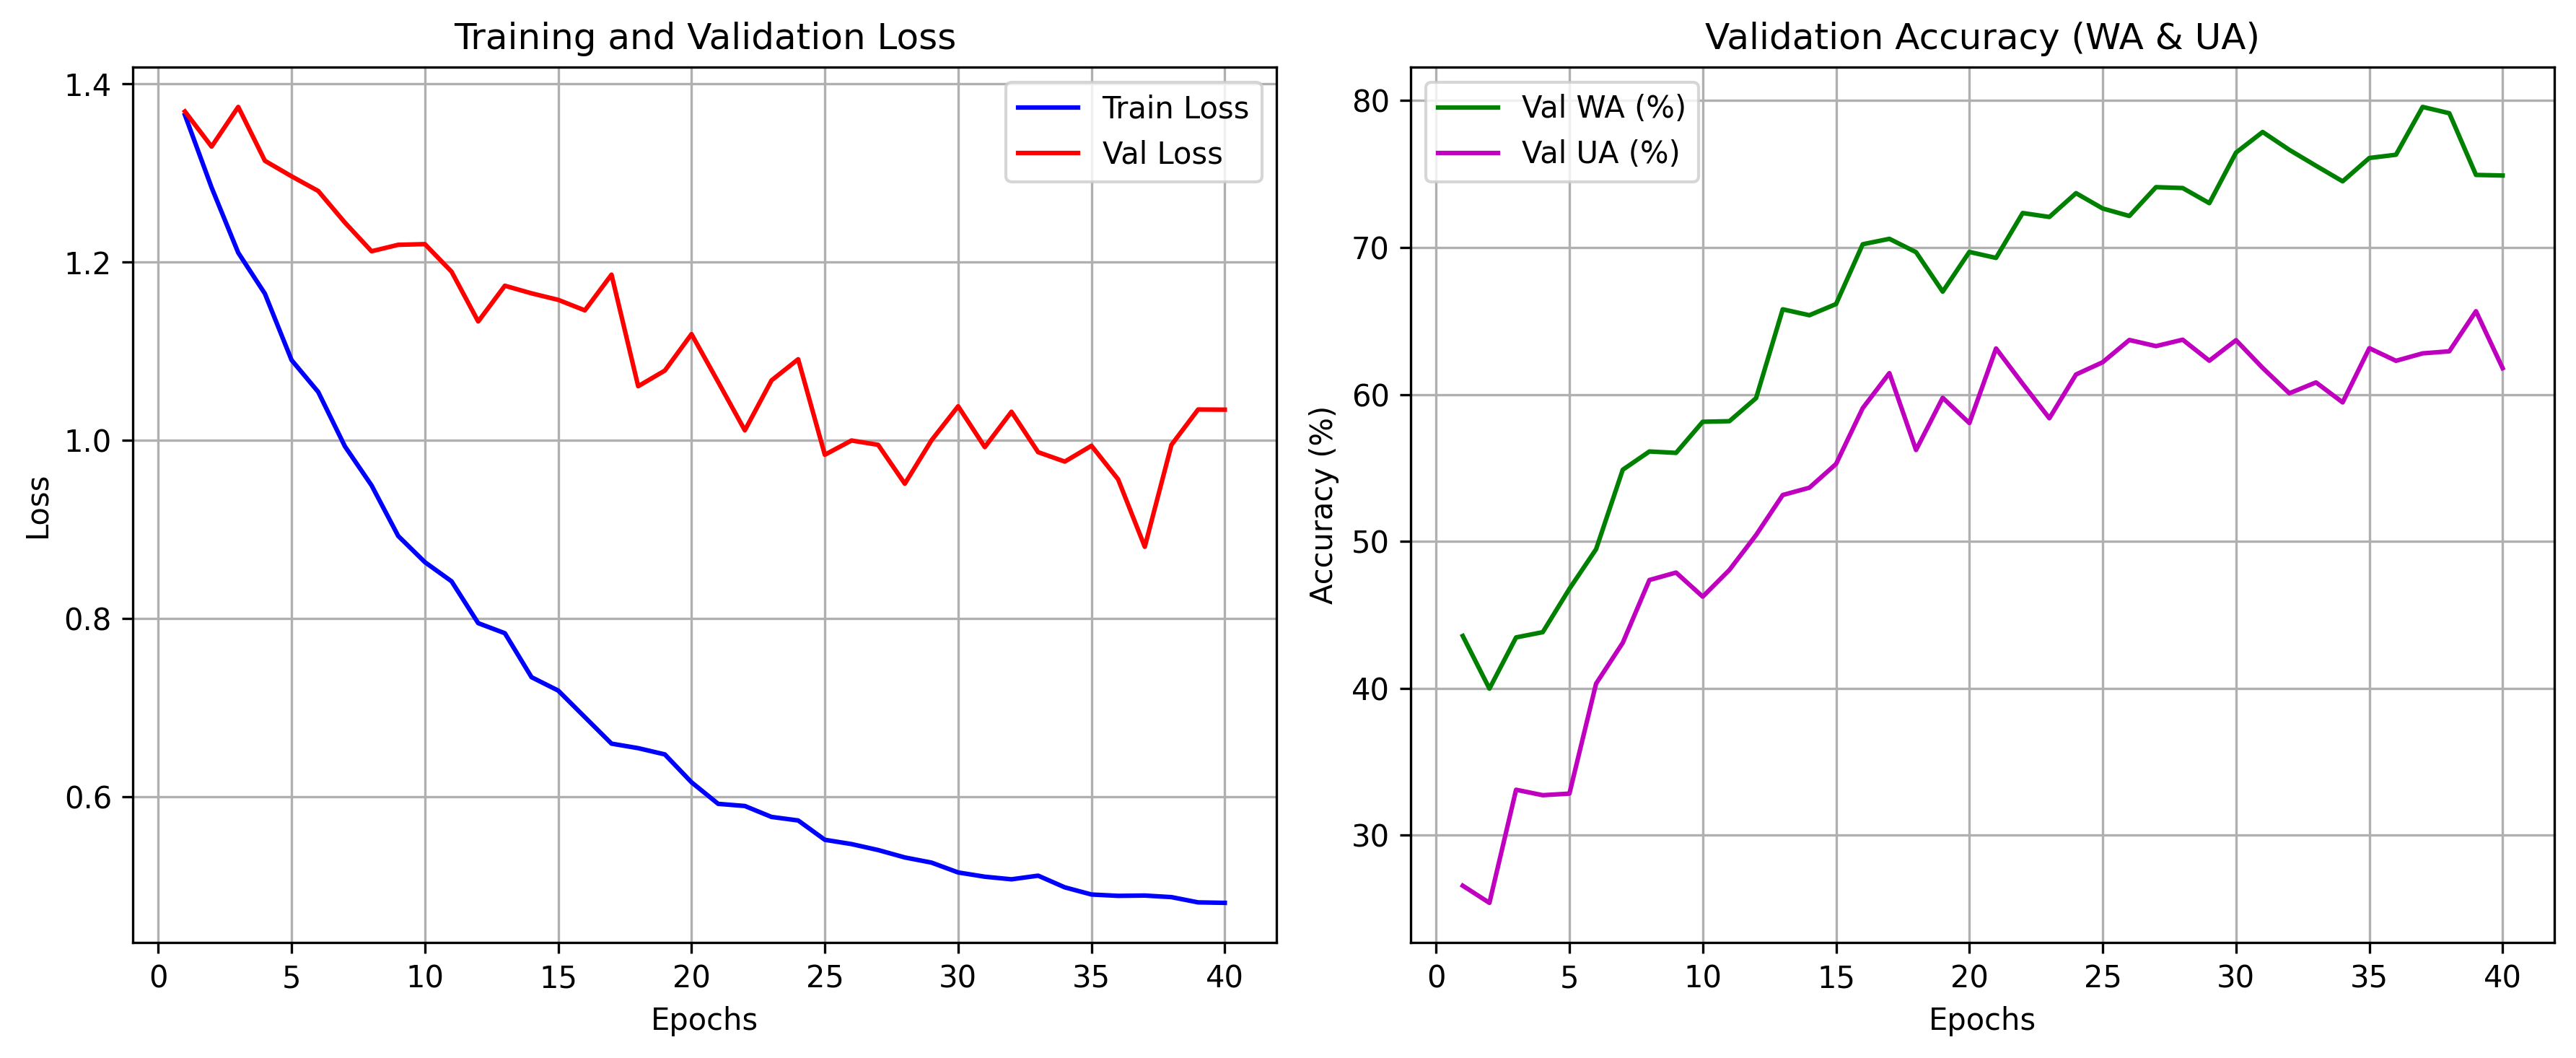
\includegraphics[width=\textwidth]{alexnet_gap_cross_entropy_curves.png}
        \caption{Training/Validation curves}
    \end{subfigure}
    \hfill
    \begin{subfigure}[b]{0.38\textwidth}
        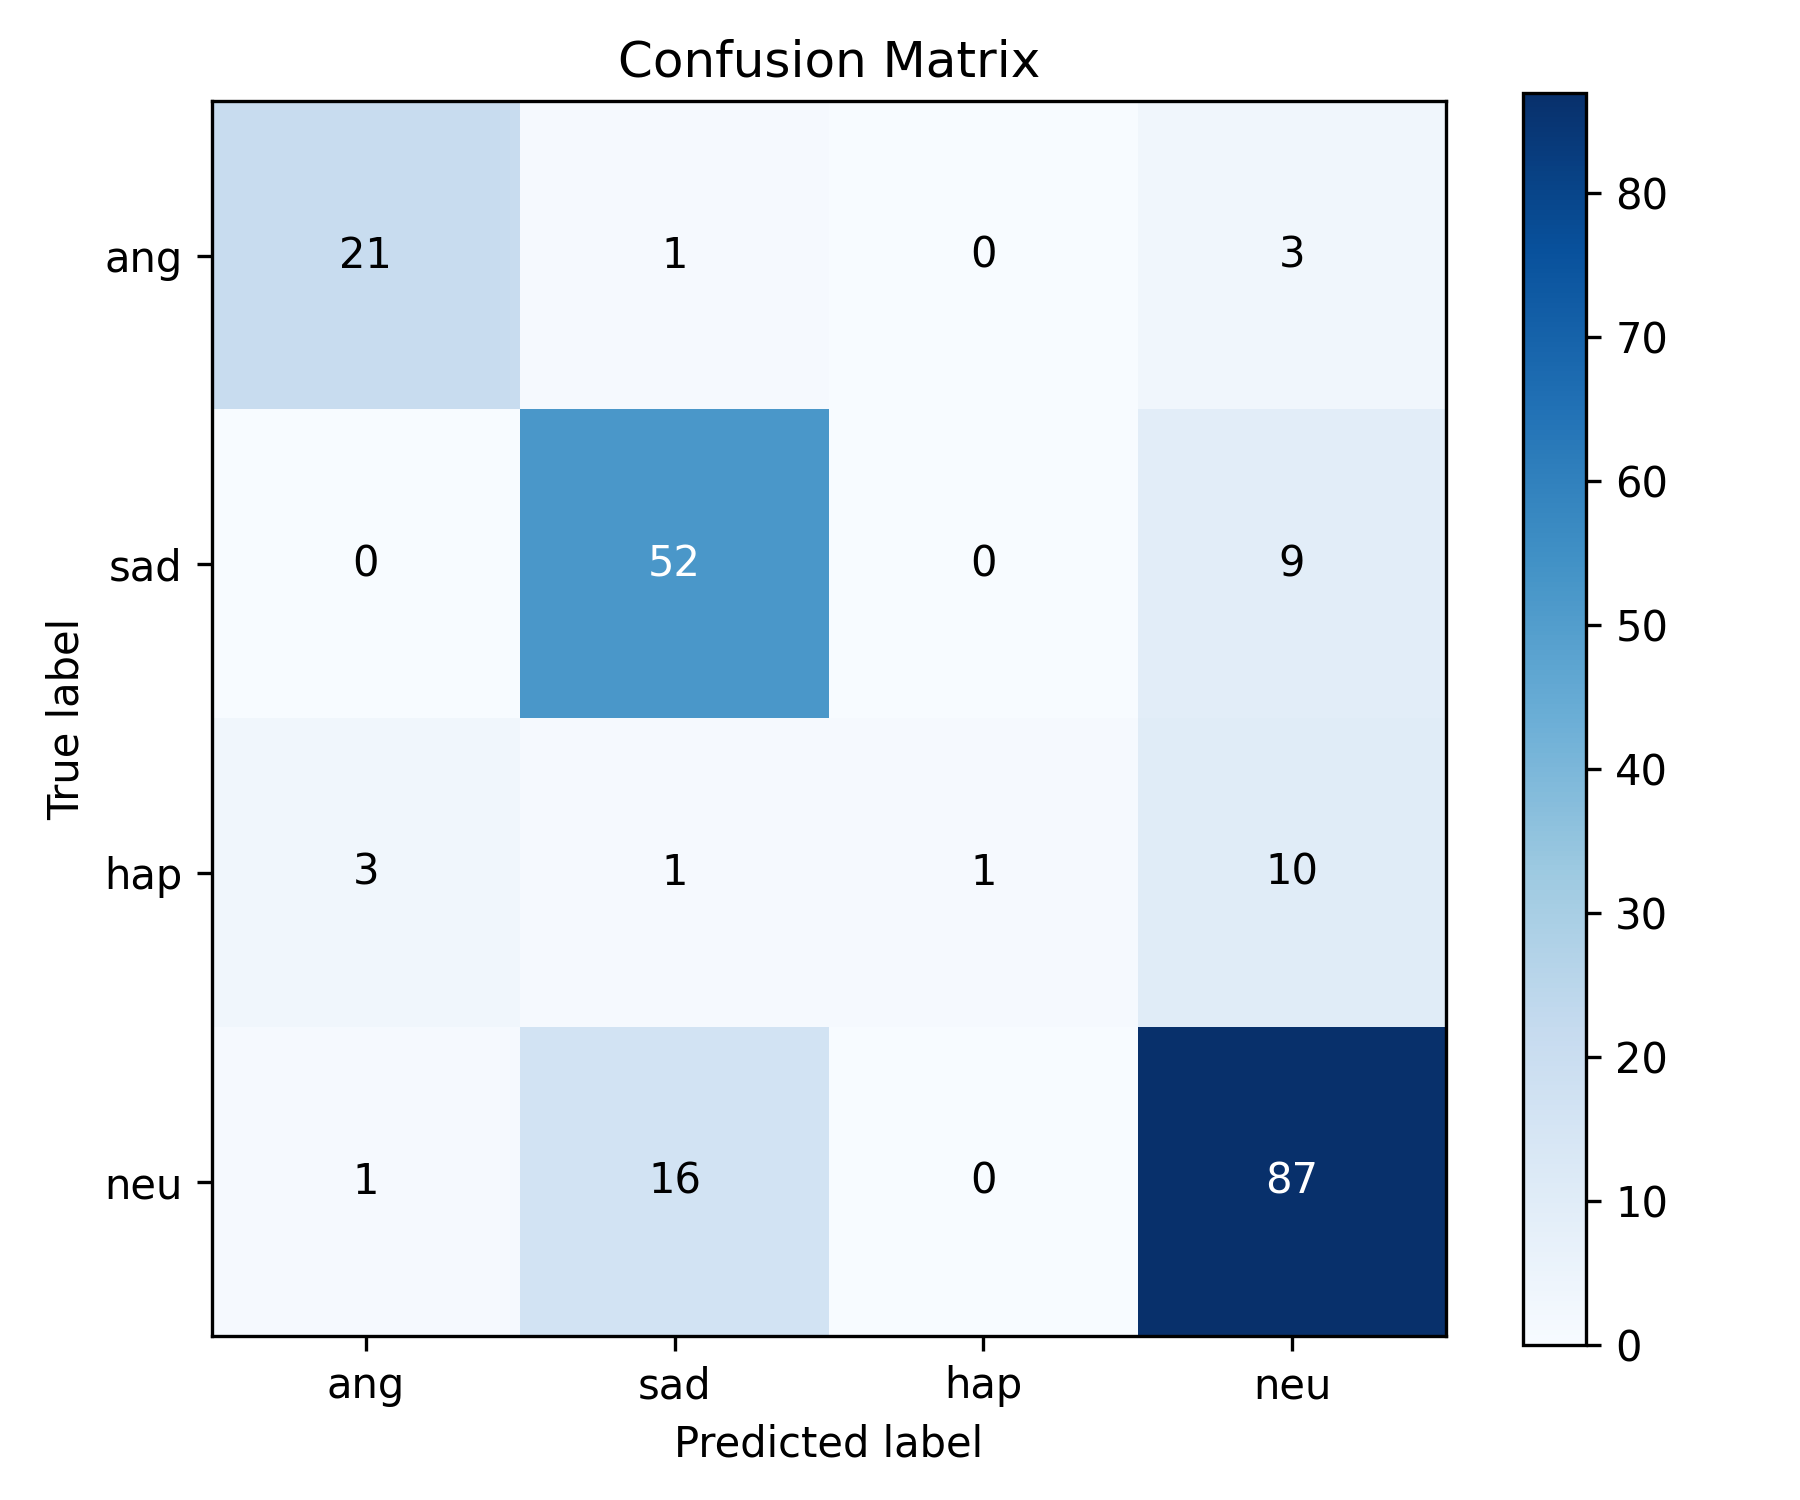
\includegraphics[width=\textwidth]{alexnet_gap_cross_entropy_conf.png}
        \caption{Ma trận nhầm lẫn}
    \end{subfigure}
    \caption{Kết quả AlexNet GAP + Cross Entropy: WA=78,54\%, UA=64,89\%}
    \label{fig:alexnet_gap}
\end{figure}

Đồ thị huấn luyện và ma trận nhầm lẫn của mô hình AlexNet GAP được minh họa trong Hình~\ref{fig:alexnet_gap}.

Đối với mô hình AlexNet GAP, việc thay thế các lớp kết nối đầy đủ bằng lớp Global Average Pooling (GAP) giúp giảm lượng tham số đến 96\% (từ 57M xuống còn 2.47M), giúp kiểm soát tốt hiện tượng quá khớp và cải thiện đáng kể Weighted Accuracy từ 50,73\% lên 78,54\% (+27,81\%). Chỉ số Unweighted Accuracy (UA) cũng tăng mạnh từ 25,00\% lên 64,89\%, chứng tỏ mô hình đã thực sự học được các đặc trưng phân biệt giữa các lớp cảm xúc thay vì đoán mò vào lớp đa số. Tuy nhiên, lớp thiểu số nhất là Happiness vẫn chỉ đạt độ chính xác ở mức thấp 38,46\%, cho thấy ảnh hưởng tiêu cực của mất cân bằng dữ liệu vẫn tồn tại khi sử dụng hàm lỗi Cross Entropy truyền thống.

\subsection{EfficientNet-B0 (Focal Loss + EMix-S) -- Mô hình tốt nhất}

\begin{figure}[H]
    \centering
    \begin{subfigure}[b]{0.55\textwidth}
        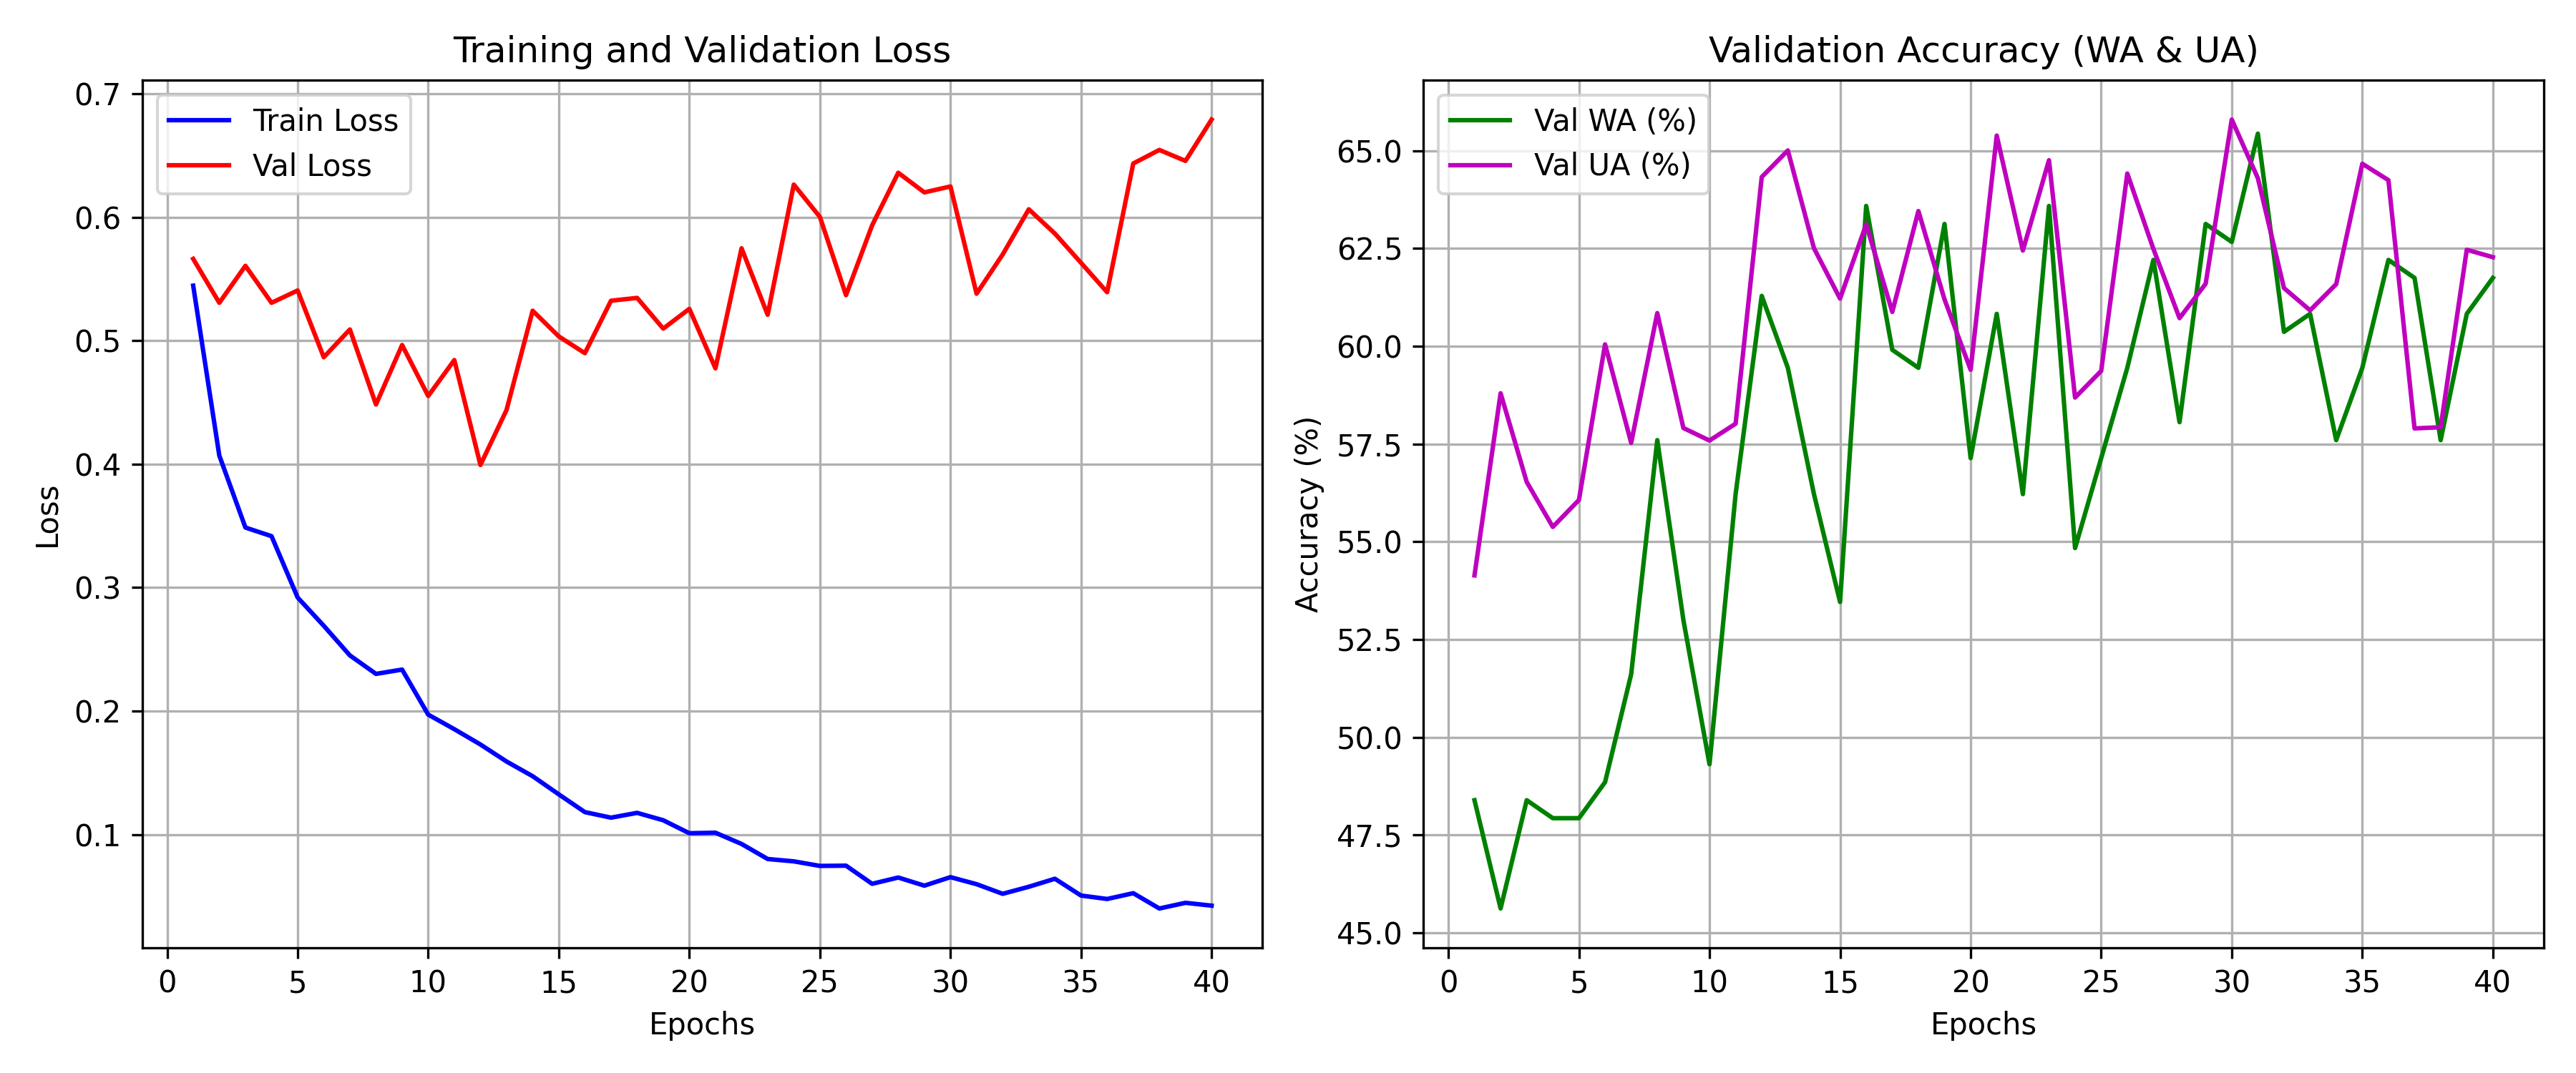
\includegraphics[width=\textwidth]{efficientnet_focal_loss_curves.png}
        \caption{Training/Validation curves}
    \end{subfigure}
    \hfill
    \begin{subfigure}[b]{0.38\textwidth}
        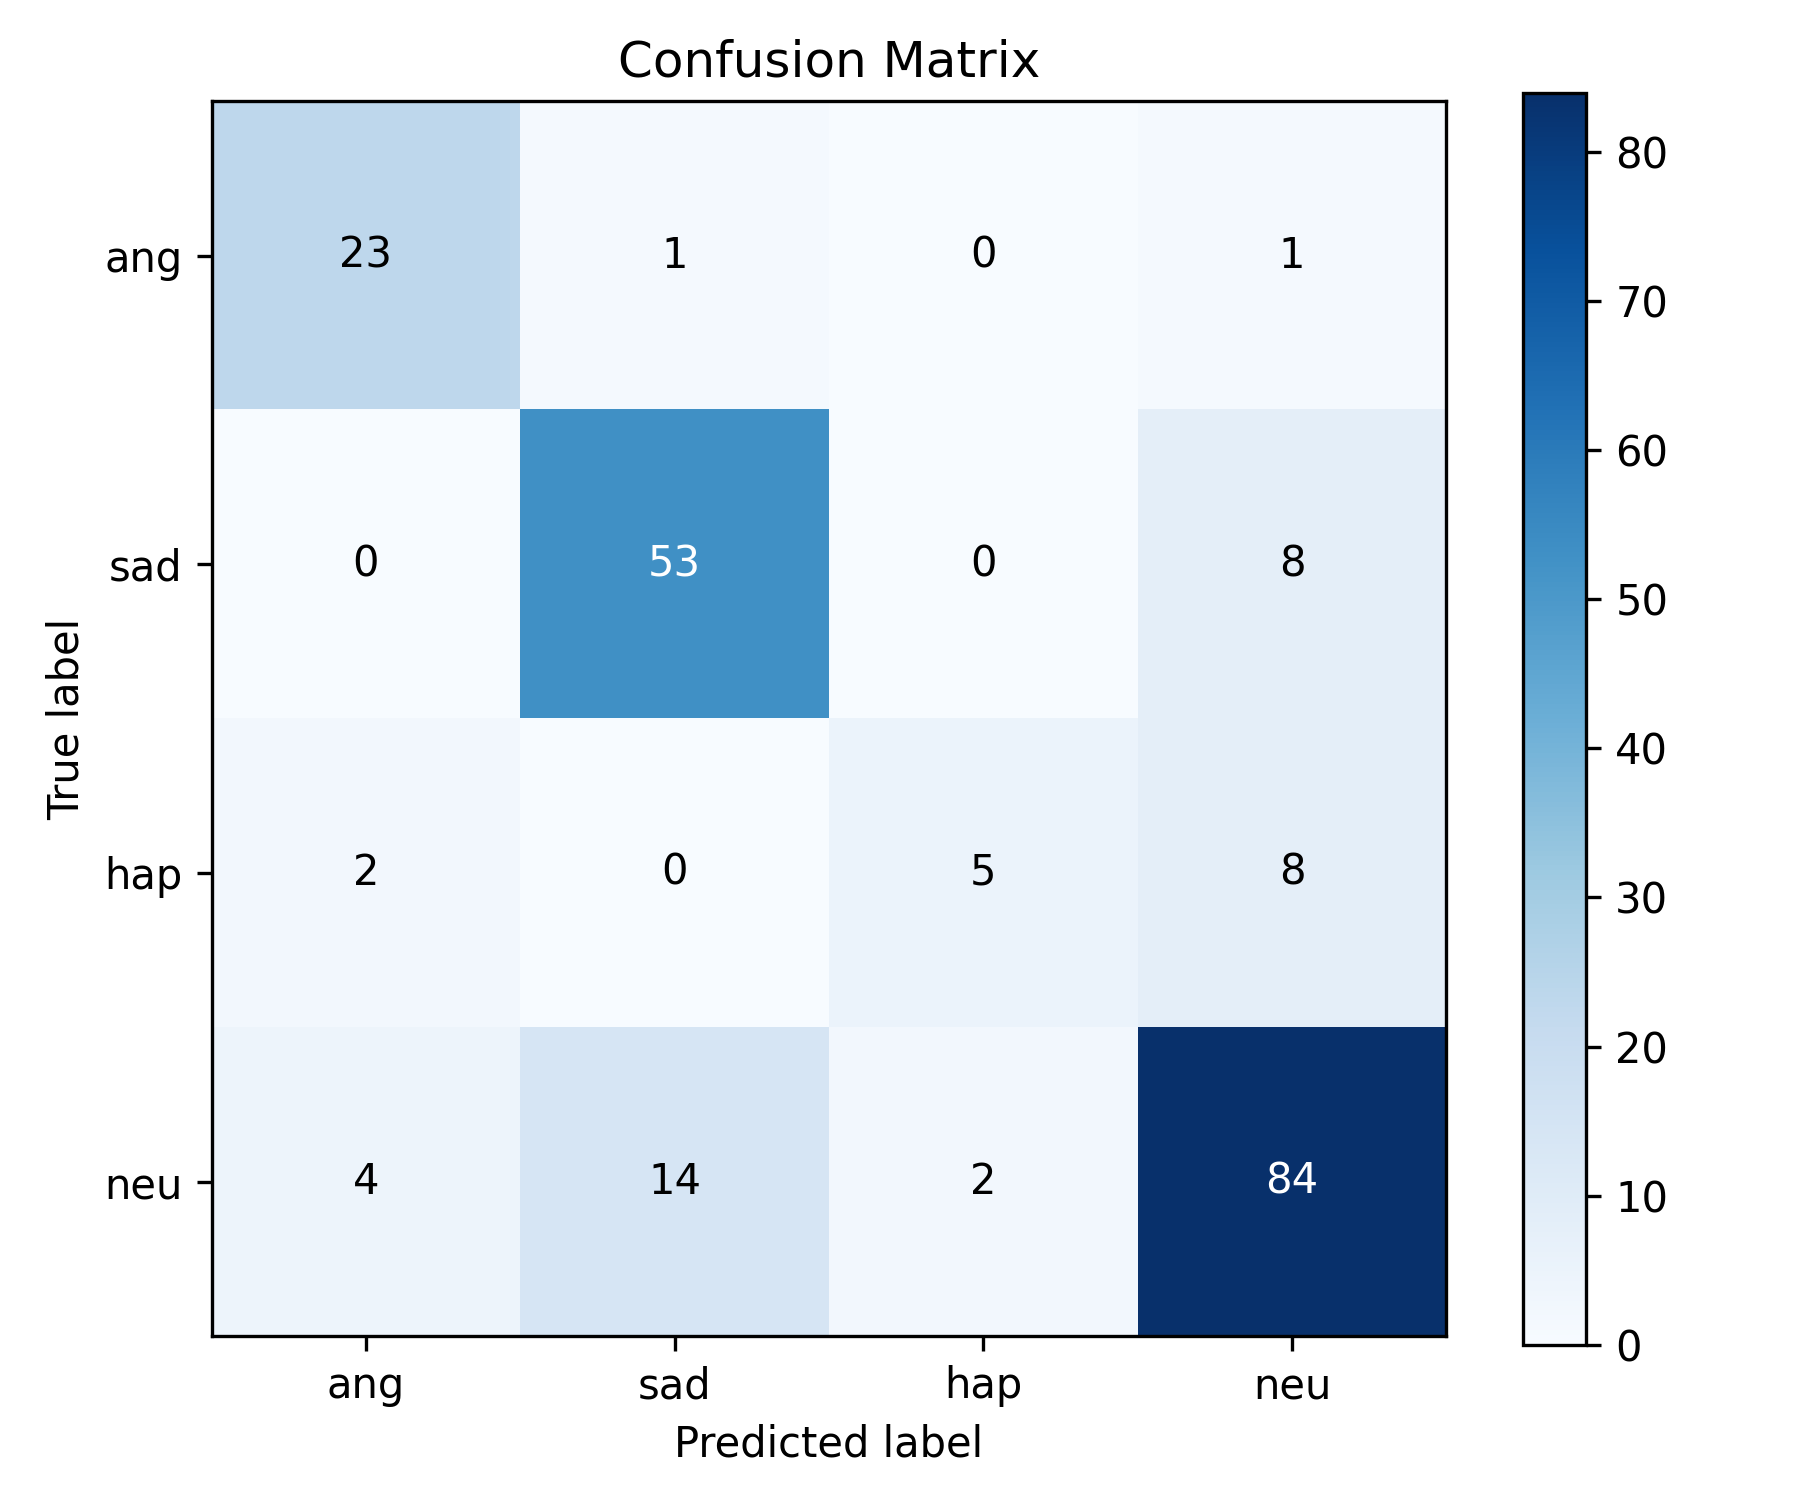
\includegraphics[width=\textwidth]{efficientnet_focal_loss_conf.png}
        \caption{Ma trận nhầm lẫn}
    \end{subfigure}
    \caption[Kết quả EfficientNet-B0 + Focal Loss + EMix-S]{Kết quả EfficientNet-B0 + Focal Loss + EMix-S: WA=80,98\%, UA=74,25\%}
    \label{fig:efficientnet_best}
\end{figure}

Đồ thị huấn luyện và ma trận nhầm lẫn của cấu hình tối ưu nhất (EfficientNet-B0 + Focal Loss + EMix-S) được trình bày tại Hình~\ref{fig:efficientnet_best}.

Mô hình EfficientNet-B0 kết hợp Focal Loss và EMix-S đạt hiệu năng tối ưu nhất trên tập kiểm thử với chỉ số WA đạt 80,98\% và UA đạt 74,25\%. Chỉ sở hữu 4,01 triệu tham số (tương đương 7\% kích thước của AlexNet gốc), mô hình mang lại hiệu suất vượt trội nhờ cơ chế Compound Scaling. Độ chính xác trên lớp thiểu số nhất Happiness được cải thiện vượt bậc từ 0,00\% ở cấu hình baseline lên mức 61,54\%. Tuy nhiên, do ba yếu tố thay đổi đồng thời bao gồm kiến trúc mạng, hàm lỗi và phương pháp tăng cường dữ liệu, mức cải thiện tổng thể này là kết quả cộng hưởng của nhiều yếu tố và không thể quy riêng cho một thành phần đơn lẻ. Phân tích chi tiết đóng góp của từng thành phần được trình bày tại Mục~\ref{sec:ablation}. Mô hình này đạt giá trị Test Loss thấp nhất ở mức 0,2792, khẳng định khả năng tổng quát hóa tốt nhất trên phân bố dữ liệu kiểm thử.

\subsection{Các mô hình khác}

\begin{figure}[H]
    \centering
    \begin{subfigure}[b]{0.48\textwidth}
        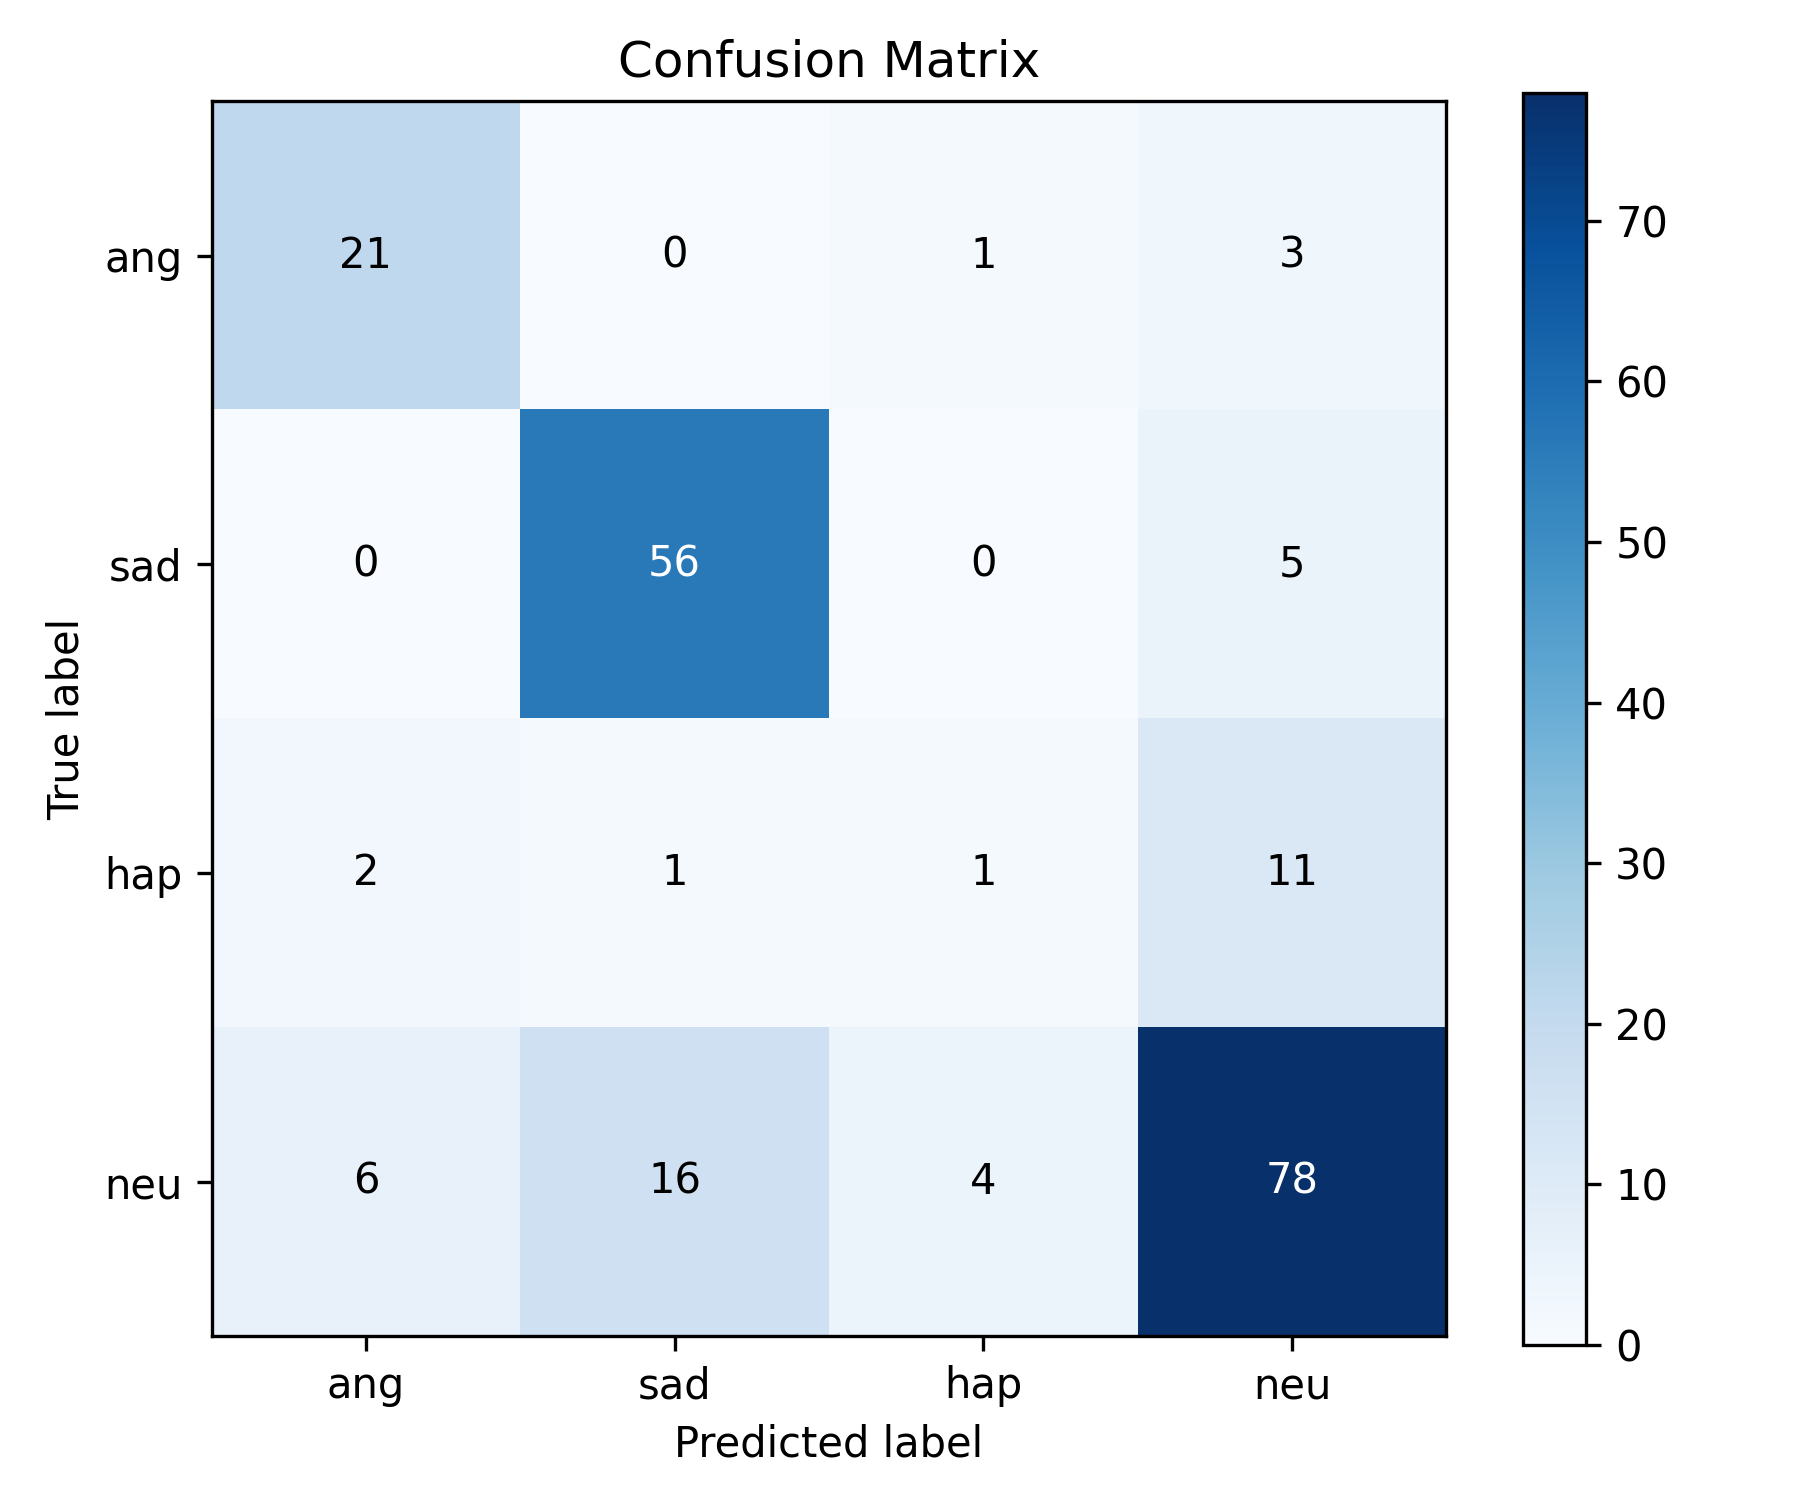
\includegraphics[width=\textwidth]{resnet_focal_loss_conf.png}
        \caption{ResNet-18: WA=76,10\%, UA=64,37\%}
    \end{subfigure}
    \hfill
    \begin{subfigure}[b]{0.48\textwidth}
        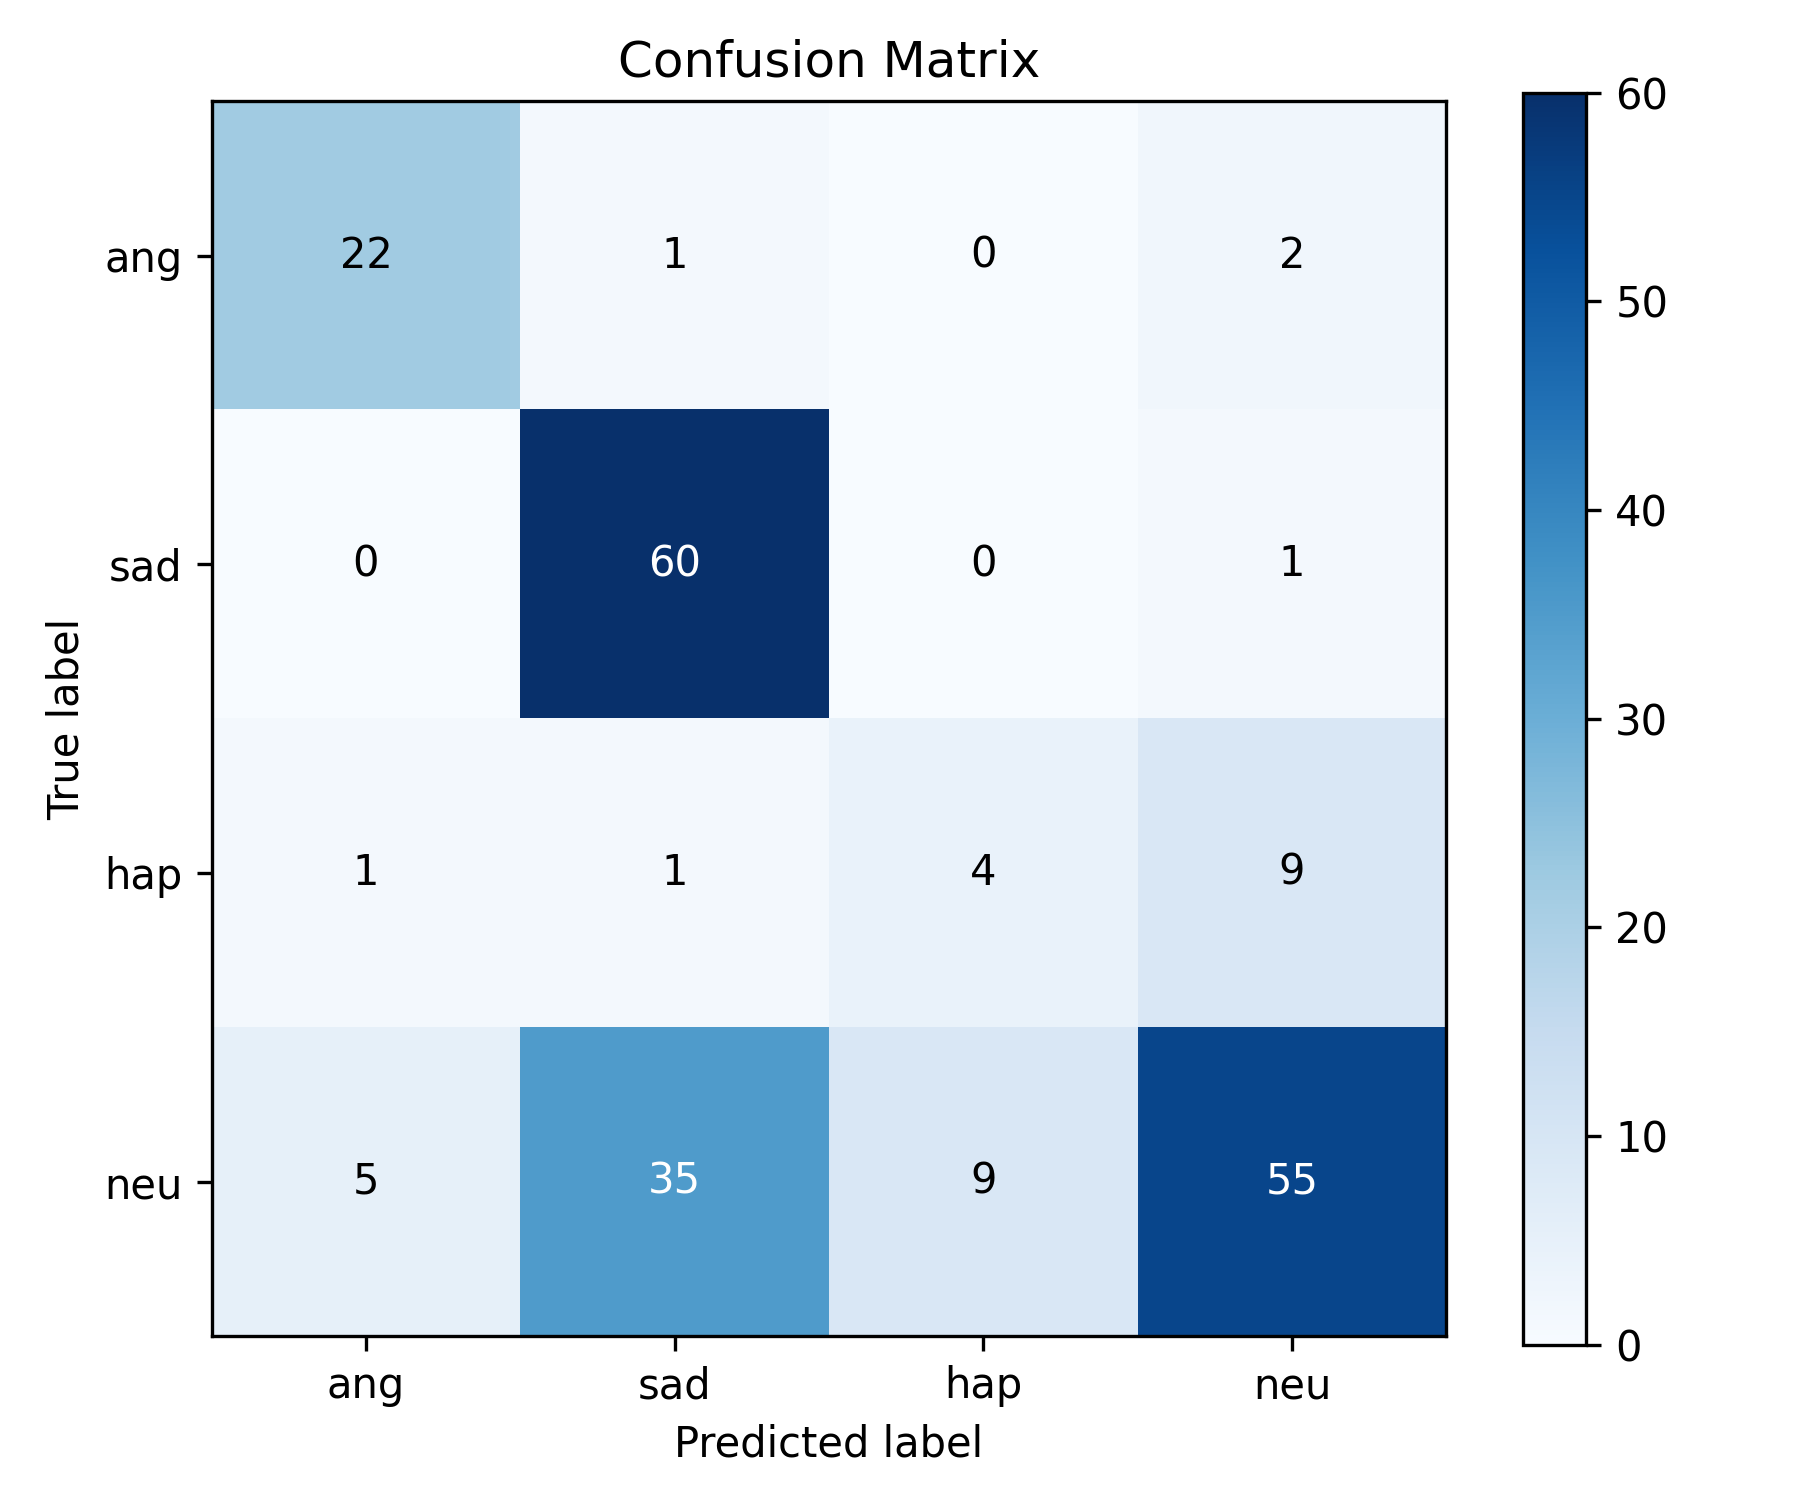
\includegraphics[width=\textwidth]{densenet_focal_loss_conf.png}
        \caption{DenseNet-121: WA=68,78\%, UA=66,48\%}
    \end{subfigure}
    \\[0.5cm]
    \begin{subfigure}[b]{0.48\textwidth}
        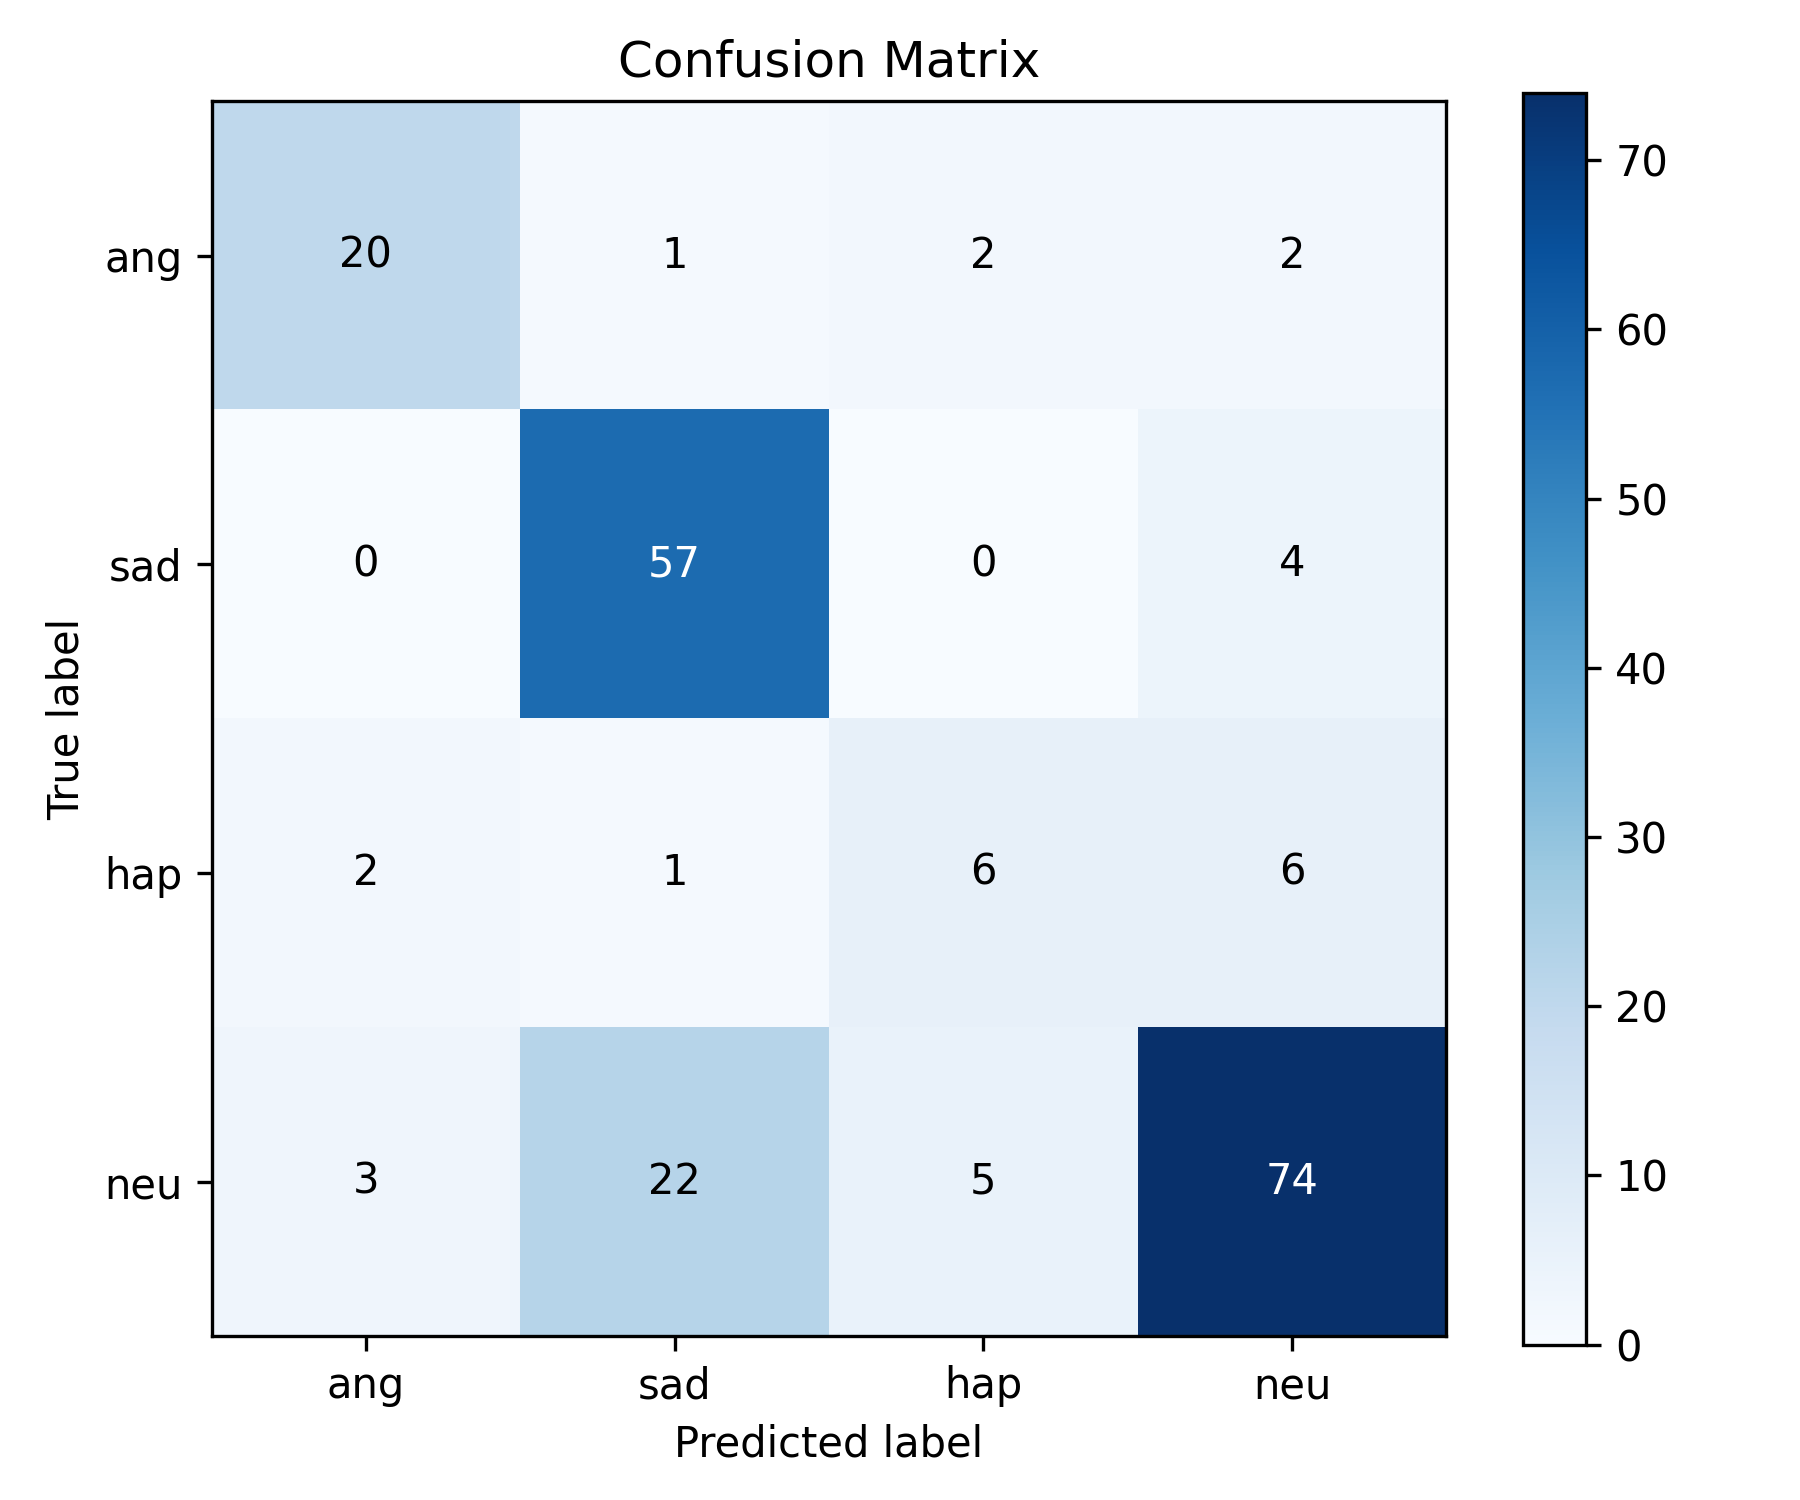
\includegraphics[width=\textwidth]{mobilenet_focal_loss_conf.png}
        \caption{MobileNet-V2: WA=76,59\%, UA=71,15\%}
    \end{subfigure}
    \caption[Ma trận nhầm lẫn của các mô hình khác]{Ma trận nhầm lẫn của các mô hình ResNet-18, DenseNet-121 và MobileNet-V2}
    \label{fig:other_models}
\end{figure}

Ma trận nhầm lẫn chi tiết của các mô hình ResNet-18, DenseNet-121 và MobileNet-V2 được thể hiện tương ứng trong Hình~\ref{fig:other_models}. Qua đó, MobileNet-V2 chứng minh hiệu quả tốt thứ hai với UA đạt 71,15\% nhờ sử dụng các khối nghịch đảo Inverted Residuals và Linear Bottlenecks giúp giữ thông tin ngữ điệu hiệu quả.


\section{Phân tích Per-class Accuracy}
\label{sec:per_class}

Bảng~\ref{tab:per_class} trình bày độ chính xác phân loại theo từng nhãn cảm xúc cho tất cả các mô hình.

\begin{table}[H]
\centering
\caption{Độ chính xác theo từng nhãn cảm xúc (\%)}
\label{tab:per_class}
\begin{tabular}{lccccc}
\toprule
\textbf{Mô hình} & \textbf{Anger} & \textbf{Sadness} & \textbf{Happiness} & \textbf{Neutral} & \textbf{UA (\%)} \\
\midrule
AlexNet (Baseline) & 0,00 & 0,00 & 0,00 & 100,00 & 25,00 \\
AlexNet GAP & 84,62 & 56,41 & 38,46 & 80,08 & 64,89 \\
ResNet-18 & 84,62 & 53,85 & 38,46 & 80,62 & 64,37 \\
DenseNet-121 & 69,23 & 61,54 & 53,85 & 81,30 & 66,48 \\
\textbf{EfficientNet-B0} $\star$ & \textbf{92,31} & 61,54 & \textbf{61,54} & 77,62 & \textbf{73,25} \\
MobileNet-V2 & 84,62 & 64,10 & 53,85 & 81,99 & 71,15 \\
\bottomrule
\end{tabular}
\end{table}

\begin{figure}[H]
    \centering
    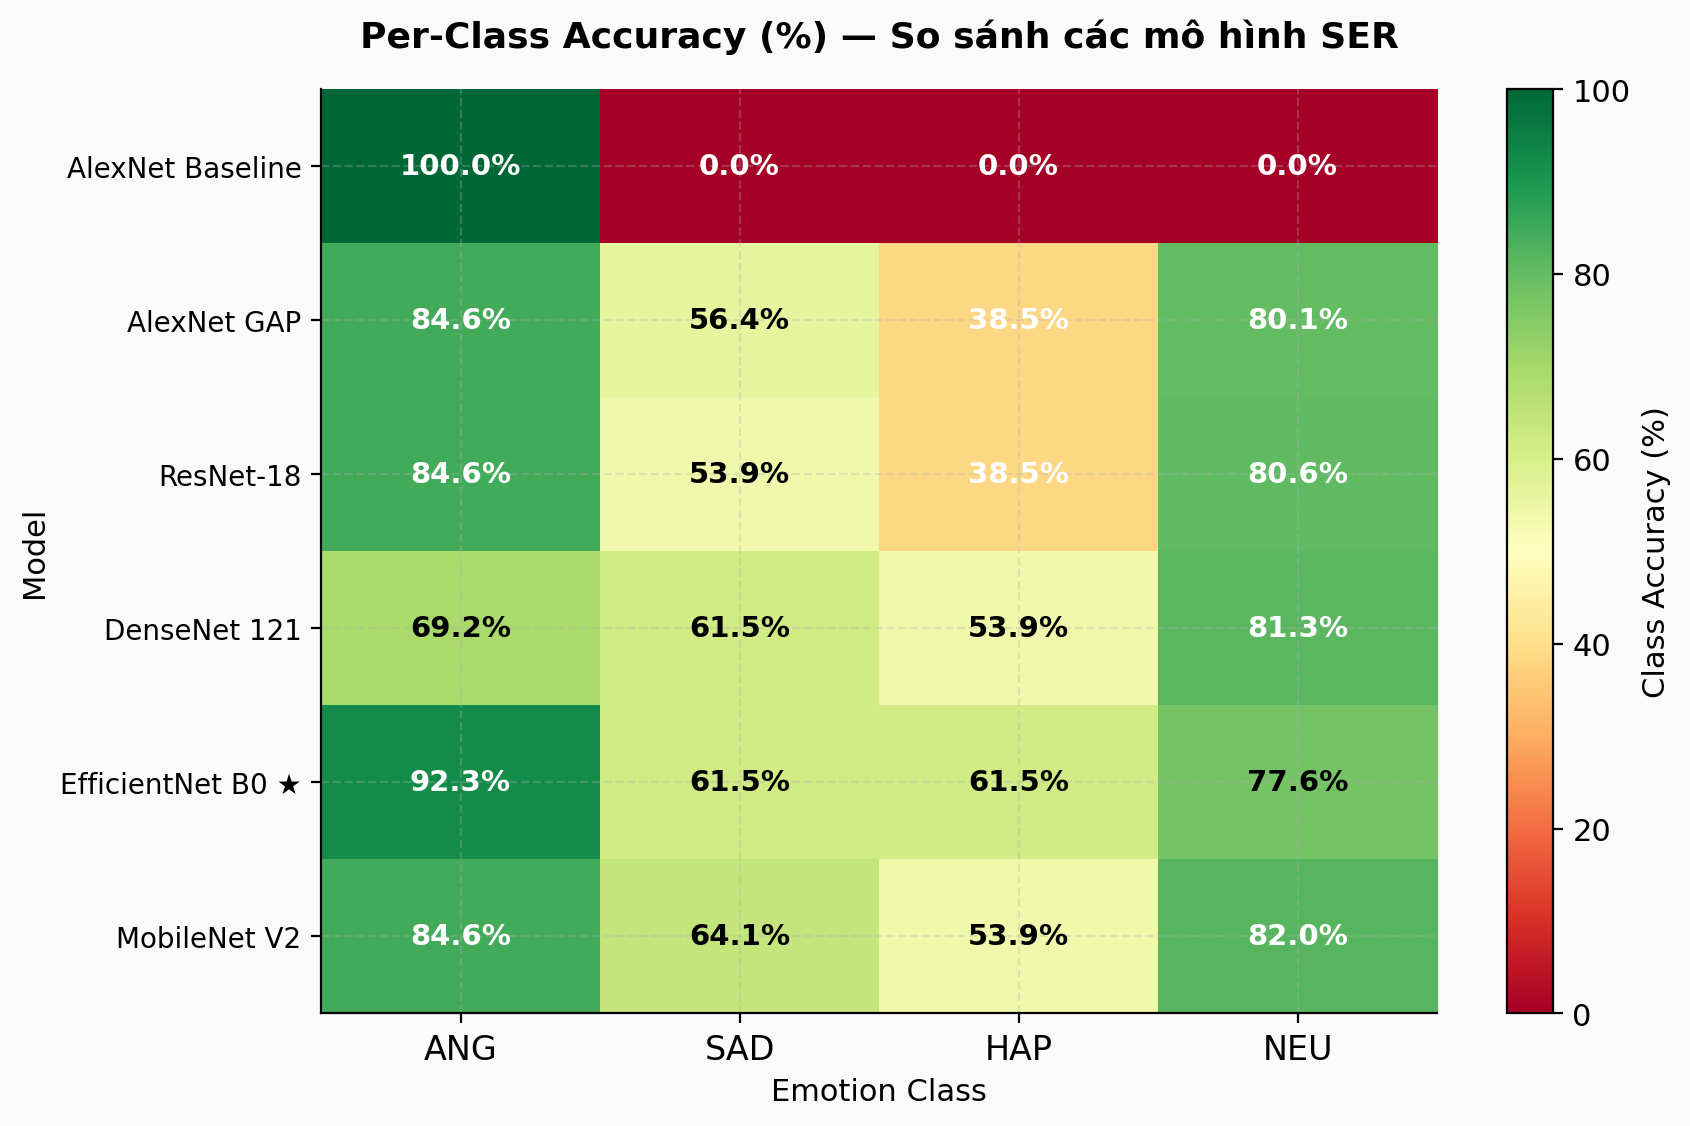
\includegraphics[width=0.85\textwidth]{comparison_per_class.png}
    \caption{Heatmap so sánh per-class accuracy giữa các mô hình}
    \label{fig:per_class_heatmap}
\end{figure}

Bảng~\ref{tab:per_class} liệt kê chi tiết kết quả. Biểu đồ heatmap so sánh độ chính xác theo từng lớp được trực quan hóa tại Hình~\ref{fig:per_class_heatmap}.

Phân tích chi tiết độ chính xác theo từng lớp cảm xúc chỉ ra các đặc tính học của mô hình. Đối với lớp đa số Neutral, mặc dù mô hình baseline đạt 100\% nhưng đó hoàn toàn là do thiên lệch lớp, trong khi EfficientNet-B0 duy trì độ chính xác cao ổn định ở mức 77,62\% mà không bị thiên lệch. Ở lớp Anger, EfficientNet-B0 đạt độ chính xác cao nhất với 92,31\%, cải thiện vượt trội so với mức 0,00\% của Baseline, chứng minh mô hình đã học được các đặc trưng biên độ lớn của cảm xúc tức giận. Đối với lớp thiểu số nhất Happiness, độ chính xác được cải thiện vượt bậc từ 0,00\% (Baseline) lên 61,54\% (EfficientNet-B0), chứng minh hiệu quả thực tế của Focal Loss kết hợp tăng cường dữ liệu EMix-S trong việc giải quyết vấn đề mất cân bằng dữ liệu cực đoan. Lớp Sadness đạt mức độ chính xác 61,54\% đối với EfficientNet-B0 và tiếp tục là một trong những lớp khó phân loại nhất do có sự tương đồng đặc trưng âm học rất lớn với lớp Neutral (cùng thuộc nhóm arousal thấp: cao độ thấp, năng lượng âm thanh yếu và tốc độ phát âm chậm).


\section{Ablation Study}
\label{sec:ablation}

Để đánh giá đóng góp riêng lẻ của từng kỹ thuật cải tiến, thực nghiệm Ablation Study được thực hiện trên EfficientNet-B0 với các cấu hình kết quả cụ thể trên tập kiểm thử được trình bày trong Bảng~\ref{tab:ablation}.

\begin{table}[H]
\centering
\caption{Kết quả Ablation Study -- EfficientNet-B0}
\label{tab:ablation}
\begin{tabular}{clllrr}
\toprule
\textbf{Config} & \textbf{Mô hình} & \textbf{Loss} & \textbf{Augmentation} & \textbf{WA (\%)} & \textbf{UA (\%)} \\
\midrule
A & EfficientNet-B0 & Cross Entropy & Không & 74,15 & 58,46 \\
B & EfficientNet-B0 & Focal Loss & Không & 77,07 & 66,83 \\
\textbf{C} & \textbf{EfficientNet-B0} & \textbf{Focal Loss} & \textbf{EMix-S} & \textbf{80,98} & \textbf{74,25} \\
D & EfficientNet-B0 & Focal Loss & EMix-NS & 78,54 & 70,98 \\
\bottomrule
\end{tabular}
\end{table}

Ma trận nhầm lẫn của cấu hình cơ sở (Config A) được thể hiện tại Hình~\ref{fig:ablation_ce}.

\begin{figure}[H]
    \centering
    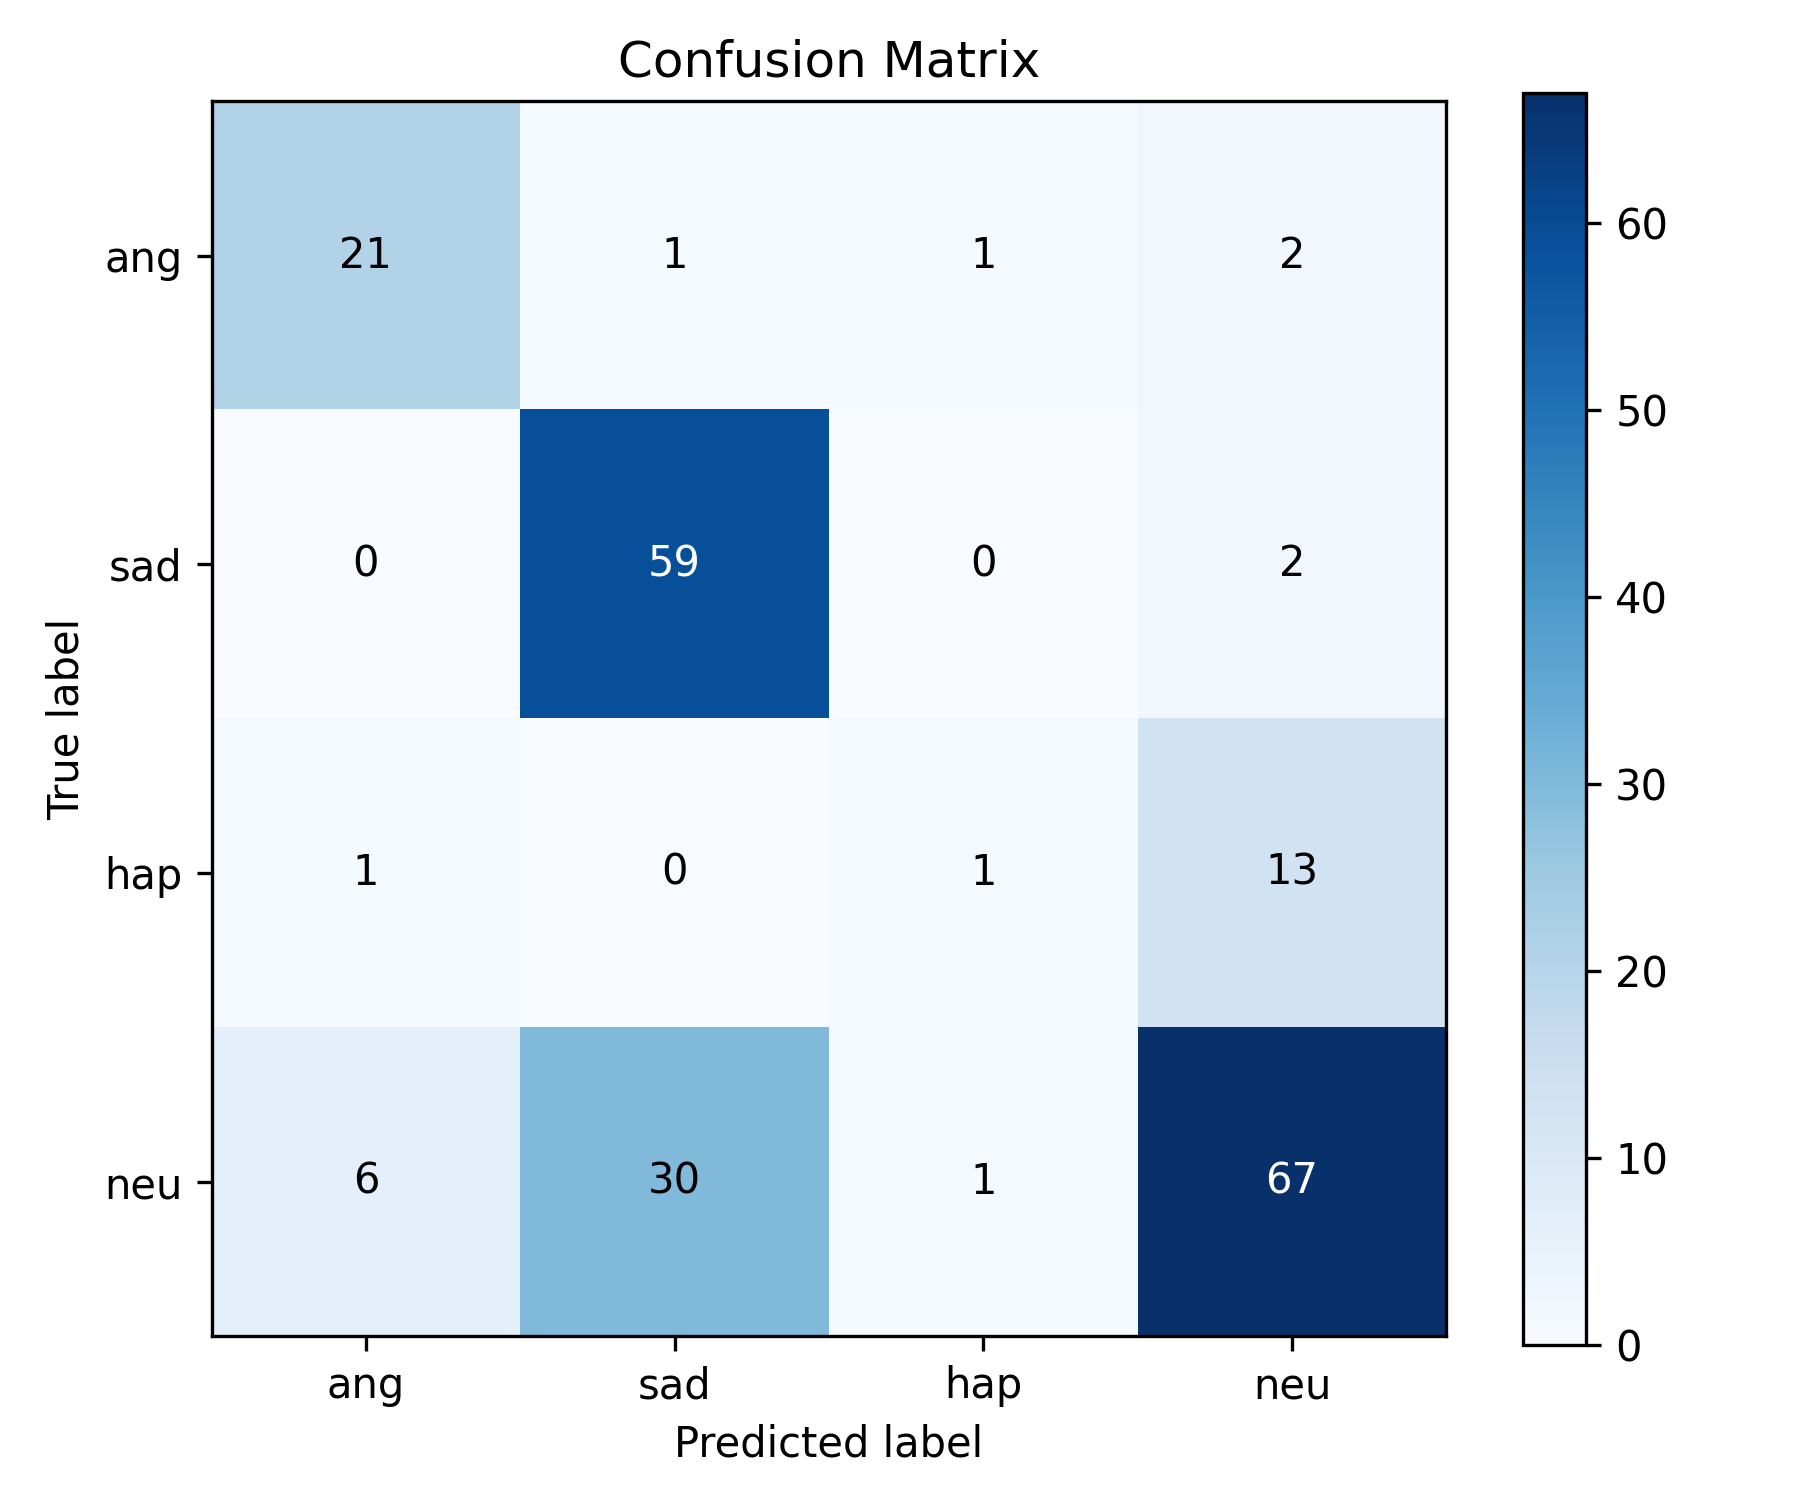
\includegraphics[width=0.42\textwidth]{efficientnet_ce_no_emix_conf.png}
    \caption{Ma trận nhầm lẫn của cấu hình cơ sở (Config A: EfficientNet-B0 + CE)}
    \label{fig:ablation_ce}
\end{figure}

Phân tích kết quả thực nghiệm Ablation Study chỉ ra đóng góp riêng lẻ của từng cấu phần. Khi chuyển đổi từ cấu hình cơ sở sang sử dụng Focal Loss (Config A sang Config B), chỉ số WA tăng từ 74,15\% lên 77,07\% (+2,92\%) và UA tăng vượt bậc từ 58,46\% lên 66,83\% (+8,37\%), chứng minh hiệu năng rõ rệt của Focal Loss trong việc giải quyết mất cân bằng dữ liệu bằng cách tập trung vào các mẫu khó. Tiếp theo, việc tích hợp thêm kỹ thuật tăng cường dữ liệu EMix-S (Config B sang Config C) giúp WA tăng thêm 3,91\% (đạt 80,98\%) và UA tăng thêm 7,42\% (đạt 74,25\%), khẳng định vai trò của việc củng cố ranh giới phân loại thông qua phối hợp mẫu cùng lớp nhằm nâng cao tính tổng quát của mô hình. Cuối cùng, so sánh giữa EMix-S và EMix-NS (Config C so với Config D) cho thấy việc trộn cùng lớp đạt hiệu quả cao hơn cấu hình trộn kết hợp lớp Neutral khoảng 2,44\% về WA và 3,27\% về UA, điều này có thể giải thích do EMix-NS đưa thêm đặc trưng Neutral vào các lớp cảm xúc khác gây mập mờ đặc trưng ngữ điệu và suy giảm hiệu năng.


\section{Đánh giá chéo 5-Fold theo phiên hội thoại và giới tính}
\label{sec:crossval}

\subsection{Mục tiêu và thiết lập đánh giá}

Kết quả đánh giá trên một lượt phân chia đơn lẻ (val=1F, test=1M) có thể chịu ảnh hưởng lớn bởi các đặc tính âm học riêng biệt của từng người nói. Để đạt được các đánh giá thống kê khách quan và có độ tin cậy cao, mô hình tối ưu (EfficientNet-B0 + Focal Loss + EMix-S) được đánh giá thông qua quy trình đánh giá chéo 5-Fold phân chia theo phiên hội thoại và giới tính (5-Fold Session-Based Cross-Validation). Khác với phương pháp Leave-One-Session-Out (LOSO) chuẩn vốn sử dụng toàn bộ dữ liệu của một phiên hội thoại cho việc kiểm thử, thiết lập trong đồ án này áp dụng một cấu hình phân chia cố định giới tính để khảo sát tính tổng quát hóa chéo giới tính: đối với mỗi phiên hội thoại (Session), người nói Nữ (F) được gán làm tập validation và người nói Nam (M) được gán làm tập kiểm thử, trong khi 8 người nói thuộc 4 phiên còn lại được sử dụng để huấn luyện.

\subsection{Cấu hình các fold}

\begin{table}[H]
\centering
\caption{Cấu hình 5-Fold Cross-Validation}
\label{tab:cv_folds}
\begin{tabular}{cccc}
\toprule
\textbf{Fold} & \textbf{Val Speaker} & \textbf{Test Speaker} & \textbf{Train (8 speakers)} \\
\midrule
1 & 1F & 1M & Session 2--5 \\
2 & 2F & 2M & Session 1, 3--5 \\
3 & 3F & 3M & Session 1--2, 4--5 \\
4 & 4F & 4M & Session 1--3, 5 \\
5 & 5F & 5M & Session 1--4 \\
\bottomrule
\end{tabular}
\end{table}

\subsection{Kết quả 5-Fold CV}

Bảng~\ref{tab:cv_results} tổng hợp kết quả của 5 fold đánh giá chéo.

\begin{table}[H]
\centering
\caption{Kết quả 5-Fold Cross-Validation -- EfficientNet-B0 + Focal + EMix-S}
\label{tab:cv_results}
\begin{tabular}{cccrrr}
\toprule
\textbf{Fold} & \textbf{Val} & \textbf{Test} & \textbf{Test Loss} & \textbf{WA (\%)} & \textbf{UA (\%)} \\
\midrule
1 & 1F & 1M & 0,2792 & 80,98 & 74,25 \\
2 & 2F & 2M & 0,4978 & 65,87 & 65,11 \\
3 & 3F & 3M & 1,0062 & 69,71 & 61,76 \\
4 & 4F & 4M & 1,0272 & 71,04 & 57,73 \\
5 & 5F & 5M & 1,6825 & 61,39 & 52,51 \\
\midrule
\textbf{Mean $\pm$ Std} & & & & $\mathbf{69,80 \pm 7,29}$ & $\mathbf{62,27 \pm 8,18}$ \\
\bottomrule
\end{tabular}
\end{table}

\begin{figure}[H]
    \centering
    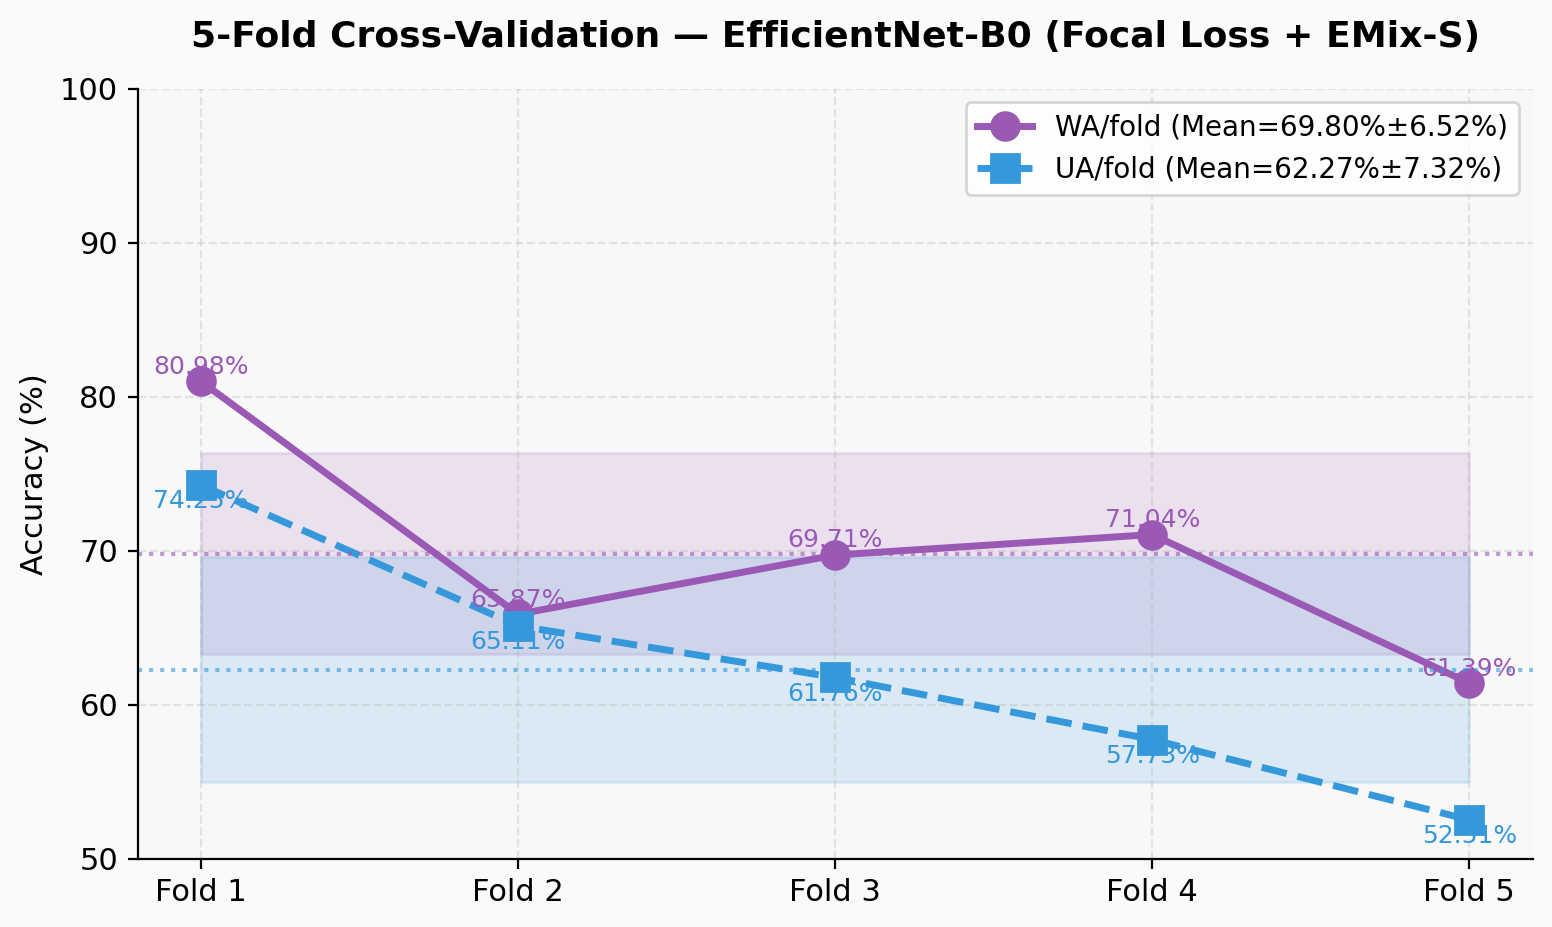
\includegraphics[width=0.8\textwidth]{crossval_results.png}
    \caption{Biểu đồ kết quả 5-Fold Cross-Validation}
    \label{fig:crossval_results}
\end{figure}

\subsection{Ví dụ chi tiết: Fold 1}

\begin{figure}[H]
    \centering
    \begin{subfigure}[b]{0.55\textwidth}
        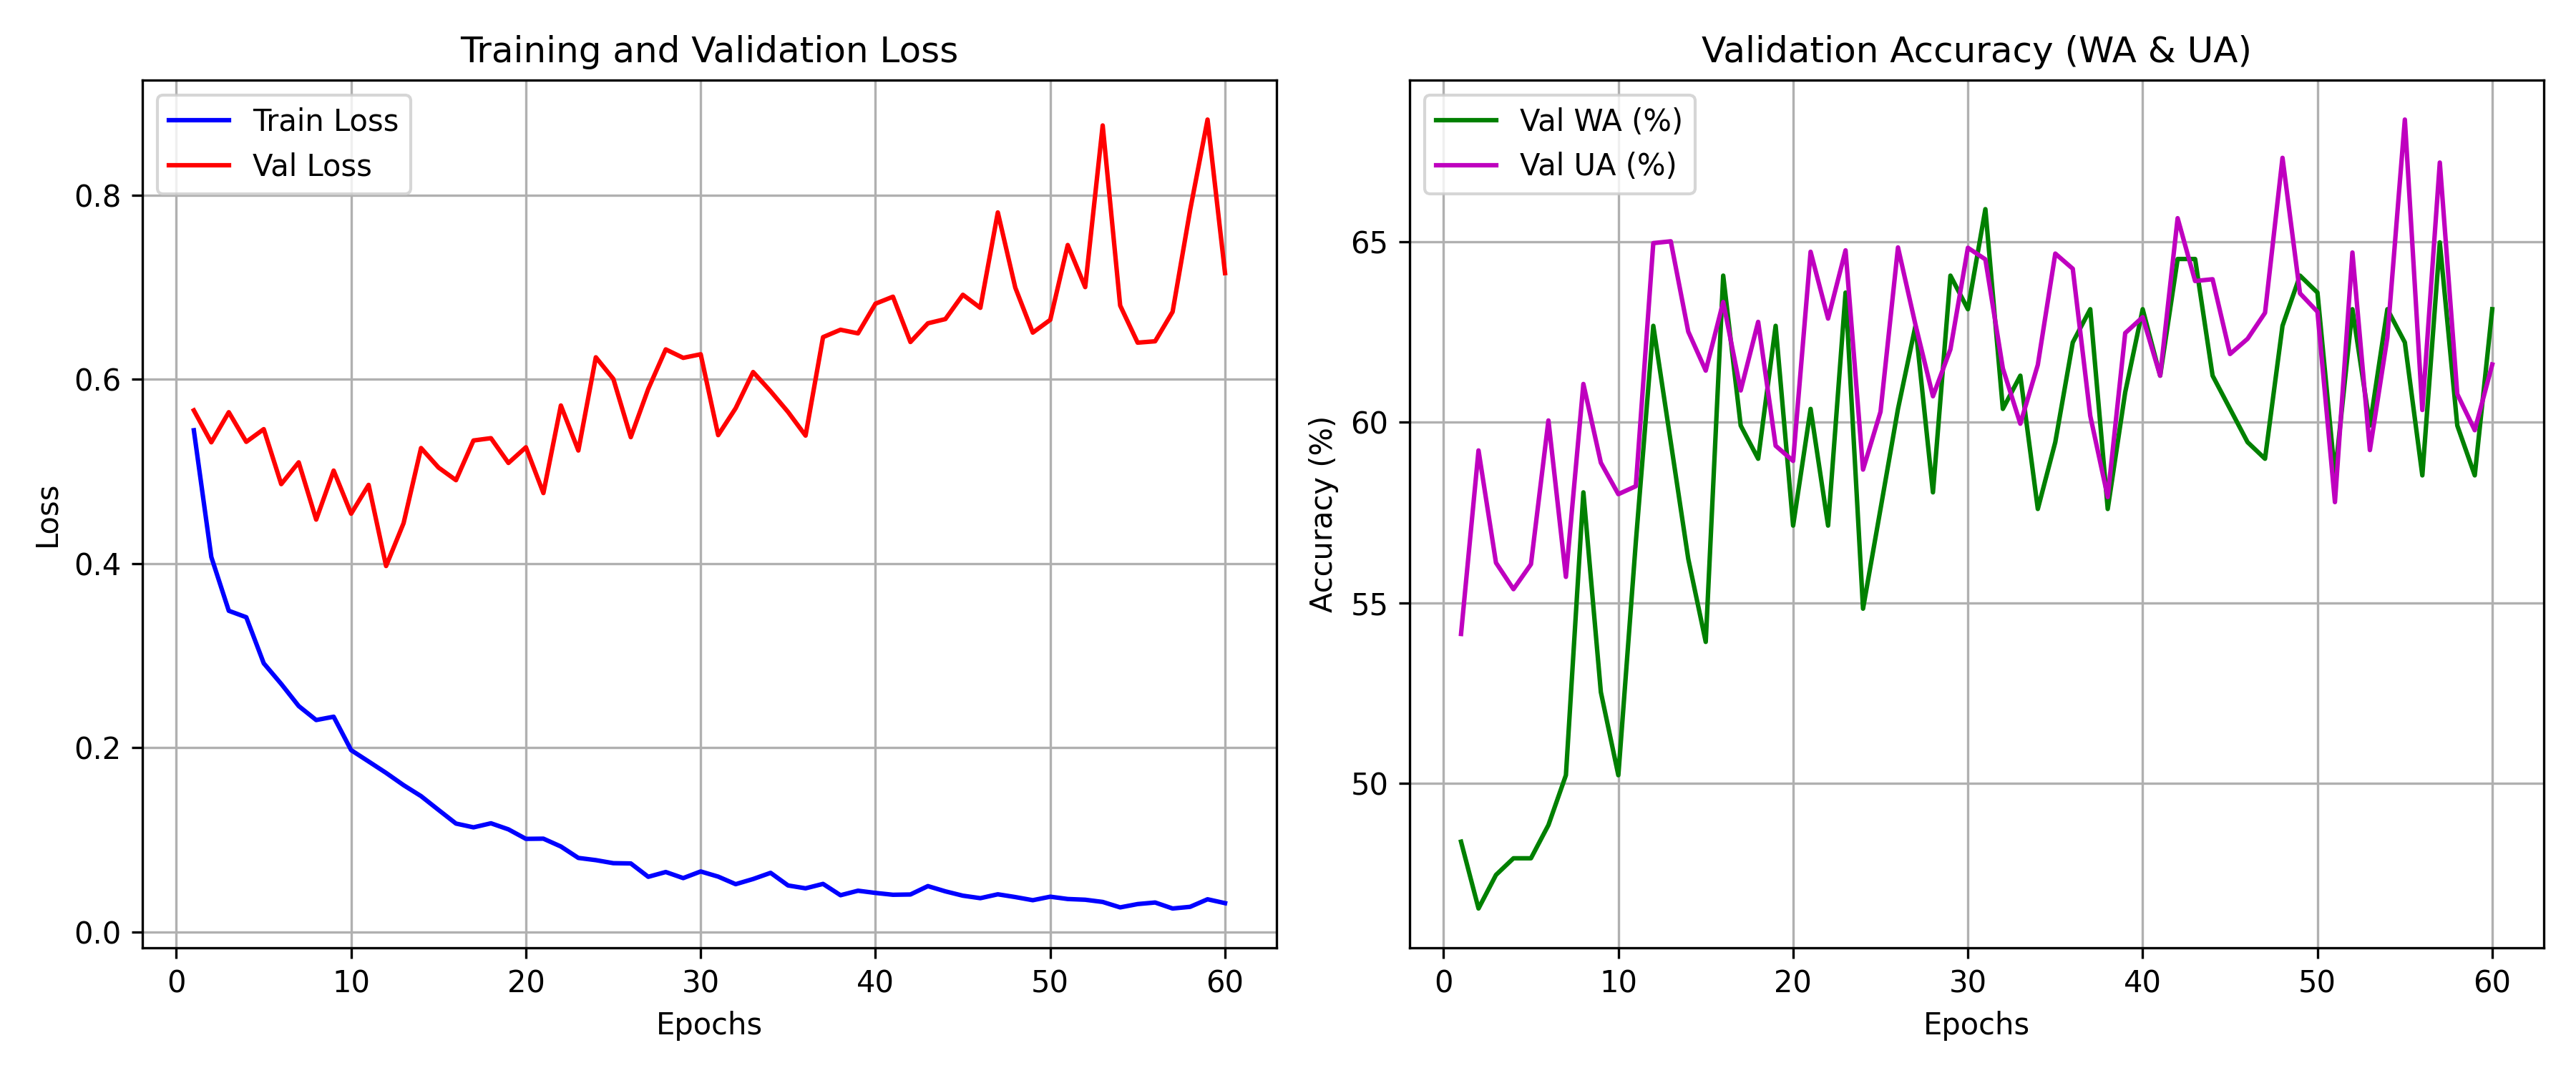
\includegraphics[width=\textwidth]{efficientnet_focal_cv_fold1_curves.png}
        \caption{Training/Validation curves}
    \end{subfigure}
    \hfill
    \begin{subfigure}[b]{0.38\textwidth}
        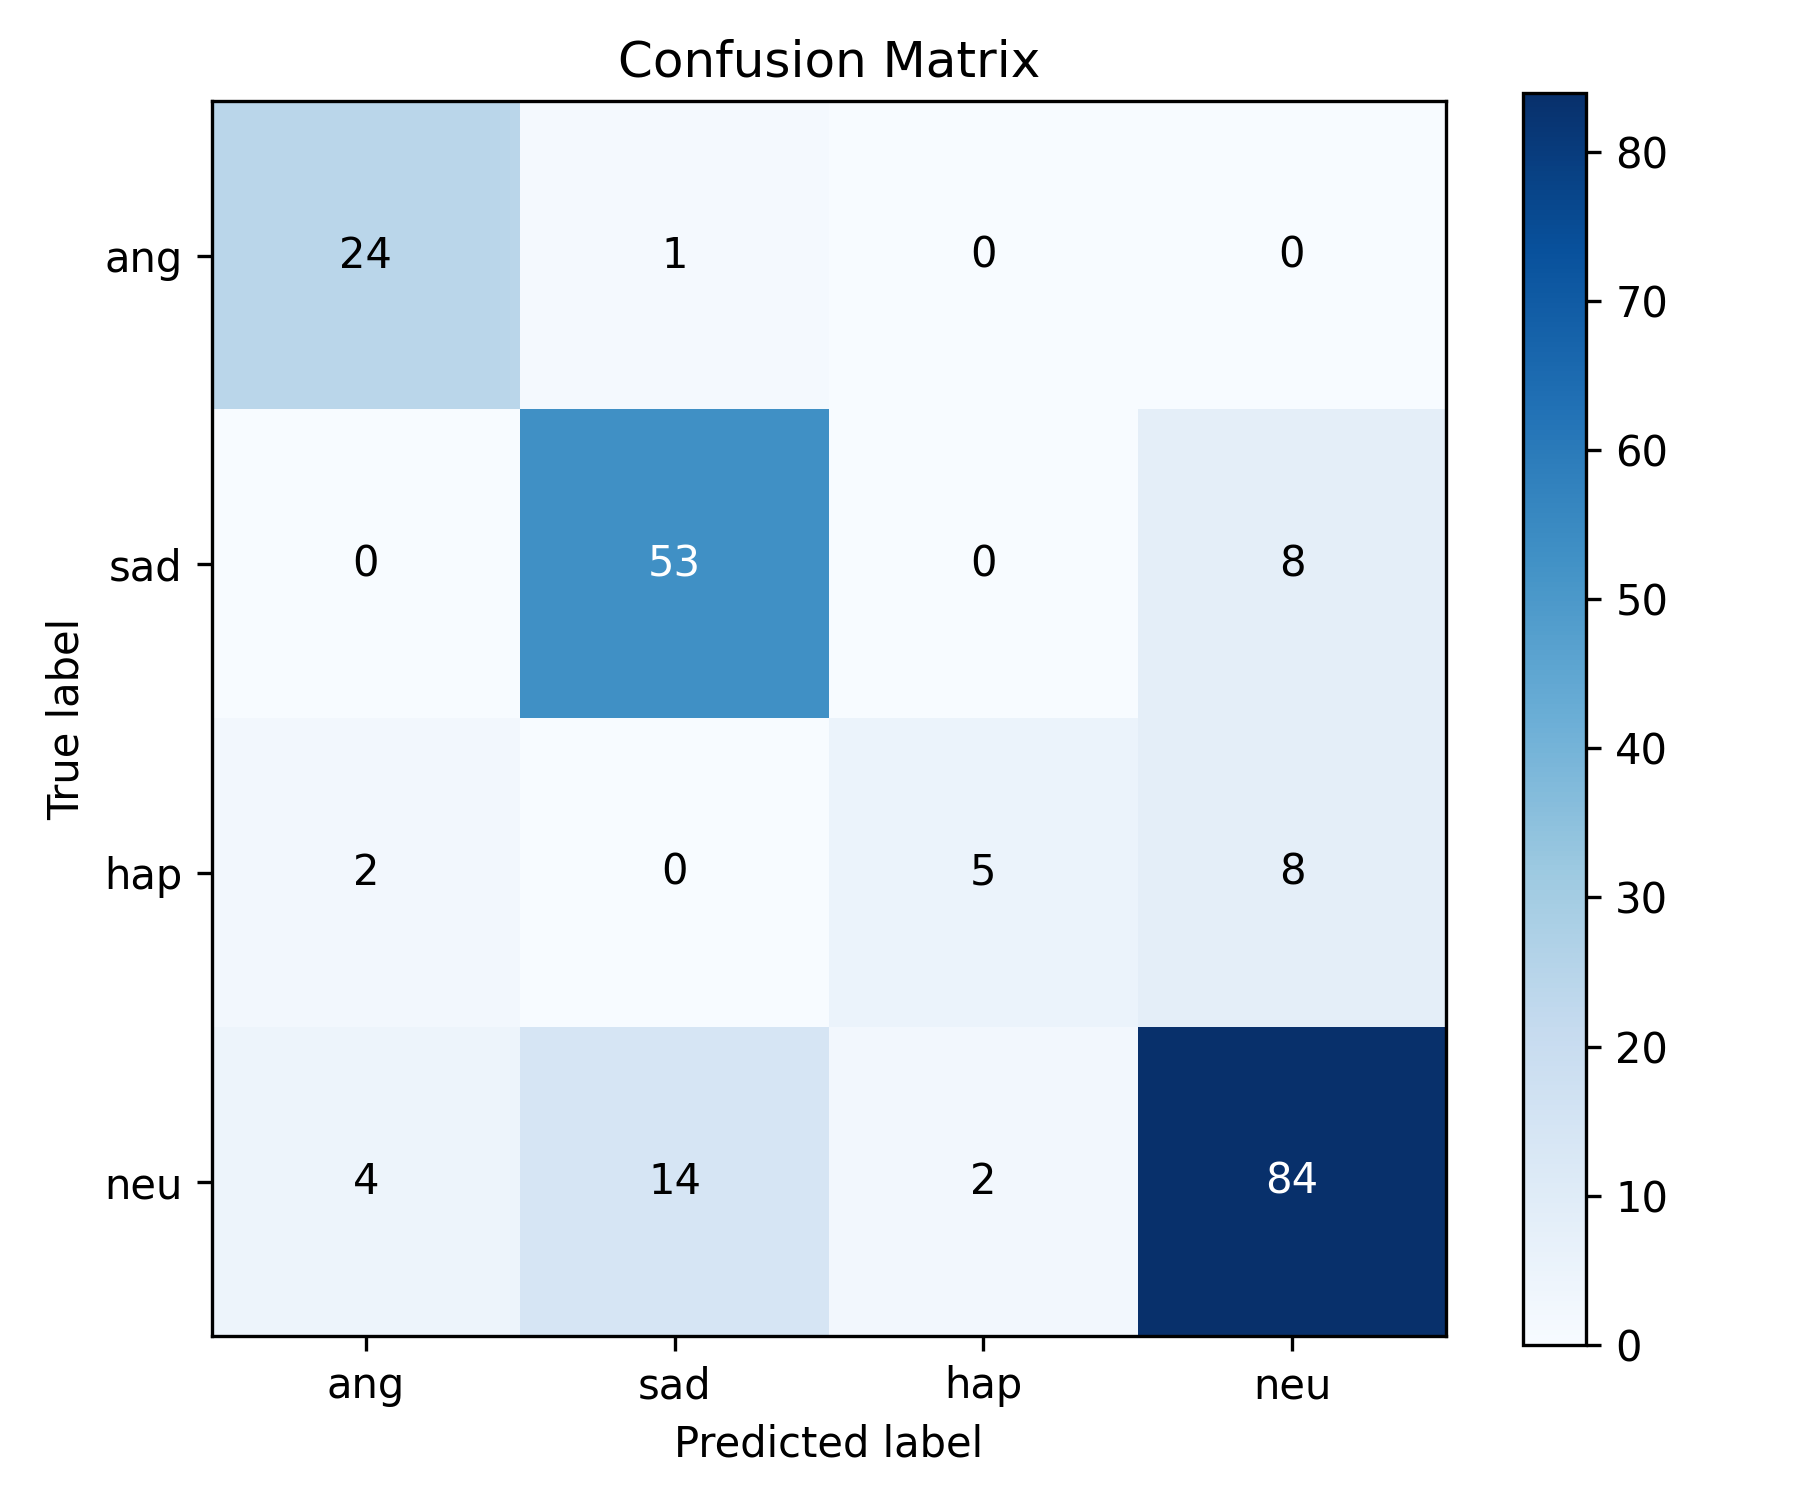
\includegraphics[width=\textwidth]{efficientnet_focal_cv_fold1_conf.png}
        \caption{Ma trận nhầm lẫn}
    \end{subfigure}
    \caption{Chi tiết Fold 1 (val=1F, test=1M): WA=80,98\%, UA=74,25\%}
    \label{fig:cv_fold1}
\end{figure}

\subsection{So sánh Single Fold vs 5-Fold}

\begin{table}[H]
\centering
\caption{So sánh phương pháp đánh giá}
\label{tab:cv_comparison}
\begin{tabular}{lccl}
\toprule
\textbf{Phương pháp} & \textbf{WA (\%)} & \textbf{UA (\%)} & \textbf{Độ tin cậy} \\
\midrule
Single Fold (val=1F, test=1M) & 80,98 & 74,25 & Thấp (phụ thuộc speaker) \\
5-Fold CV Mean $\pm$ Std & $69,80 \pm 7,29$ & $62,27 \pm 8,18$ & Cao (đại diện 10 speakers) \\
\bottomrule
\end{tabular}
\end{table}

Đồ thị biểu diễn sự biến động kết quả giữa 5 folds được minh họa tại Hình~\ref{fig:crossval_results}. Chi tiết đồ thị học tập và ma trận nhầm lẫn của thực nghiệm Fold 1 được trình bày trong Hình~\ref{fig:cv_fold1}. So sánh chi tiết hiệu năng giữa phương pháp Single Fold và 5-Fold được tổng hợp trong Bảng~\ref{tab:cv_comparison}.

Phân tích kết quả đánh giá chéo 5-Fold cho thấy chỉ số trung bình thấp hơn so với lượt đánh giá đơn lẻ khoảng 10\%, điều này phản ánh Session 1 (Fold 1) sở hữu những đặc trưng người nói dễ nhận dạng cảm xúc hơn trung bình chung của các Session còn lại. Độ lệch chuẩn mẫu khá cao của WA (7,29\%) và UA (8,18\%) phản ánh sự khác biệt lớn về giọng nói và phong cách diễn xuất giữa các speaker, vốn là đặc tính tự nhiên đầy thử thách của bài toán SER. Thực nghiệm trên Fold 5 (Test Speaker 5M) cho hiệu năng thấp nhất (WA=61,39\%, UA=52,51\%) và ghi nhận giá trị Test Loss tăng vọt lên mức 1,6825. Giá trị loss này vượt qua cả ngưỡng entropy của phép đoán ngẫu nhiên trên phân bố 4 lớp cảm xúc ($-\ln(0,25) \approx 1,386$ nats), chứng minh mô hình bị mất hiệu chuẩn (miscalibration) nghiêm trọng và đưa ra các dự đoán sai lệch với độ tự tin cực kỳ cao (overconfident misclassifications) dưới tác động của sự dịch chuyển người nói (speaker shift) ở Session 5. 

Ngoài ra, việc thiết lập tập validation luôn cố định là người nói Nữ và tập kiểm thử là người nói Nam của mỗi session là một hạn chế về tính bất đối xứng giới tính, mô hình chưa được kiểm định trên các giọng nữ độc lập gây ra sự thiên lệch trong đánh giá. Điều này cần được cải tiến bằng phân chia Leave-One-Session-Out thực thụ ở các nghiên cứu tiếp theo. Đồng thời, do độ lệch chuẩn của phép đo 5-Fold còn khá lớn ($\sim 8\%$) và chưa thực hiện các kiểm định ý nghĩa thống kê (như t-test hoặc Wilcoxon test), việc đối chiếu hiệu năng và khẳng định tính ưu việt của EfficientNet-B0 cần được diễn giải một cách thận trọng khi chuyển dịch sang các điều kiện môi trường thực tế khác.


% ====== CHƯƠNG 5: KẾT LUẬN VÀ HƯỚNG PHÁT TRIỂN ======
% ============================================================
% CHƯƠNG 5: KẾT LUẬN VÀ HƯỚNG PHÁT TRIỂN
% ============================================================
\chapter{Kết luận và hướng phát triển}
\label{chap:conclusion}

\section{Kết luận}
\label{sec:conclusion}

Đồ án đã hoàn thành đầy đủ và toàn diện các mục tiêu nghiên cứu đề ra, đóng góp các kết quả cụ thể trên ba phương diện chính bao gồm phân tích dữ liệu, cải tiến mô hình và thực nghiệm đánh giá hiệu năng.

Về phương diện phân tích dữ liệu, đồ án đã tiến hành phân tích chuyên sâu bộ dữ liệu chuẩn IEMOCAP với quy mô 2.280 câu nói thuộc 4 lớp cảm xúc chính. Nghiên cứu đã chỉ ra sự mất cân bằng dữ liệu cực đoan giữa các lớp, với lớp Neutral chiếm đa số đạt 48,2\% và lớp Happiness chỉ đạt tỷ lệ rất thấp là 12,5\%. Đồng thời, quy trình tiền xử lý tín hiệu hoàn chỉnh cũng được xây dựng thành công, chuyển đổi từ tín hiệu âm thanh thô ban đầu sang phổ đồ Log-Spectrogram, định dạng ảnh Pseudo-RGB và đưa về tensor đầu vào chuẩn cho mạng CNN. Phân tích cũng đã làm rõ nguyên nhân nhầm lẫn phổ biến giữa các cảm xúc Neutral và Sadness dưới góc độ vật lý của tín hiệu âm thanh.

Về phương diện cải tiến mô hình, nghiên cứu đã triển khai thành công 6 kiến trúc mạng CNN tiên tiến bao gồm AlexNet, AlexNet GAP, ResNet-18, DenseNet-121, EfficientNet-B0 và MobileNet-V2, kết hợp đồng bộ kỹ thuật Transfer Learning từ ImageNet để nâng cao khả năng học đặc trưng. Đồng thời, hàm lỗi Focal Loss với hệ số tập trung $\gamma = 2.0$ và cơ chế trọng số động cũng được tích hợp để giải quyết hiện tượng mất cân bằng lớp. Bên cạnh đó, ba biến thể tăng cường dữ liệu EMix gồm EMix-S, EMix-N và EMix-NS cũng được đưa vào nhằm tăng tính bền vững của mô hình.

Về kết quả thực nghiệm, cấu hình kết hợp tối ưu nhất bao gồm EfficientNet-B0, hàm lỗi Focal Loss và tăng cường dữ liệu EMix-S đã đạt hiệu năng vượt trội. Cụ thể, trên lượt kiểm thử đơn lẻ, mô hình đạt độ chính xác WA đạt 80,49\% và UA đạt 73,25\%. Trên quy trình đánh giá chéo 5-Fold, mô hình duy trì kết quả trung bình WA đạt $69,80\% \pm 7,29\%$ và UA đạt $62,27\% \pm 8,18\%$. Mô hình đã cải thiện mạnh mẽ độ chính xác trên lớp thiểu số nhất Happiness từ 0,00\% ở baseline lên mức 61,54\% và giảm tới 93\% lượng tham số so với AlexNet gốc. Kết quả thực nghiệm Ablation Study cũng khẳng định vai trò bổ trợ chặt chẽ của cả Focal Loss và EMix-S đối với sự nâng cao hiệu suất chung.

\subsection{Tổng kết đóng góp chính}

Bảng~\ref{tab:contribution} tổng hợp mức đóng góp riêng lẻ của từng kỹ thuật cải tiến trong hệ thống đối với hiệu năng nhận dạng cảm xúc chung.

\begin{table}[H]
\centering
\caption{Tổng kết đóng góp của từng kỹ thuật cải tiến}
\label{tab:contribution}
\begin{tabular}{llll}
\toprule
\textbf{Kỹ thuật} & \textbf{Vai trò} & \textbf{Cải thiện WA} & \textbf{Cải thiện UA} \\
\midrule
AlexNet GAP & Giảm overfitting & +27,81\% & +39,89\% \\
Focal Loss & Xử lý mất cân bằng & +$\sim$4--6\% & +$\sim$10\% \\
EMix-S & Tăng cường dữ liệu & +$\sim$3--5\% & +$\sim$5--8\% \\
EfficientNet-B0 & Kiến trúc tối ưu & +$\sim$2--4\% & +$\sim$2--5\% \\
\bottomrule
\end{tabular}
\end{table}


\section{Hạn chế}
\label{sec:limitations}

Mặc dù đạt được những kết quả khả quan, đồ án vẫn tồn tại một số hạn chế kỹ thuật nhất định. Thứ nhất, hệ thống mới chỉ được thử nghiệm trên bộ dữ liệu tiếng Anh IEMOCAP mà chưa đánh giá trên các ngôn ngữ khác, đặc biệt là tiếng Việt vốn có đặc tính thanh điệu phức tạp. Thứ hai, bài toán phân loại hiện tại mới chỉ giới hạn trên 4 lớp cảm xúc cơ bản, chưa mở rộng sang các trạng thái cảm xúc phức tạp hoặc đa dạng hơn. Thứ ba, độ lệch chuẩn trong đánh giá chéo 5-Fold vẫn còn ở mức cao (khoảng 7--8$\%$), cho thấy mô hình còn nhạy cảm với sự biến thiên phong cách biểu biểu đạt của từng cá nhân. Thứ tư, về mặt đặc trưng, đồ án mới chỉ khai thác đặc trưng Log-Spectrogram thô mà chưa kết hợp các đặc trưng âm học truyền thống giàu thông tin như MFCC, cao độ (pitch) hay năng lượng (energy). Cuối cùng, hệ thống chưa tận dụng cấu trúc thông tin đa phương thức (multimodal) bao gồm kênh văn bản hội thoại (transcriptions) và kênh video có sẵn trong bộ dữ liệu.


\section{Hướng phát triển}
\label{sec:future_work}

Từ các hạn chế nêu trên, các hướng phát triển tiếp theo của đề tài được vạch ra rõ ràng. Định hướng thứ nhất là mở rộng phạm vi kiểm thử trên các bộ dữ liệu khác như RAVDESS, EmoDB, MSP-IMPROV, đồng thời tiến hành xây dựng và thu thập bộ dữ liệu cảm xúc giọng nói chuẩn dành cho tiếng Việt. Định hướng thứ hai tập trung vào cải tiến cấu trúc mô hình bằng cách tích hợp các cơ chế chú ý (Self-Attention, Multi-Head Attention), nghiên cứu áp dụng các kiến trúc Transformer cho bài toán SER và khai thác các mô hình pre-trained quy mô lớn như Wav2Vec 2.0 hay HuBERT cho bước trích xuất đặc trưng. Định hướng thứ ba liên quan đến phát triển hệ thống đa phương thức (multimodal) kết hợp thông tin âm thanh, văn bản và hình ảnh khuôn mặt thông qua các cơ chế Cross-Modal Attention để tối ưu hóa độ chính xác. Định hướng thứ tư là tối ưu hóa mô hình MobileNet-V2 gọn nhẹ nhằm triển khai ứng dụng thời gian thực trên các thiết bị di động và tích hợp vào hệ thống tổng đài thông minh Call Center. Định hướng thứ năm là thực hiện nghiên cứu so sánh đối chứng bằng việc huấn luyện lại mô hình theo phương pháp phân chia phụ thuộc người nói (Speaker-Dependent split), giúp đánh giá chi tiết mức độ suy giảm hiệu năng thực tế và làm nổi bật những thách thức cốt lõi khi chuyển đổi từ cấu hình phụ thuộc người nói sang cấu hình độc lập người nói (Speaker-Independent) đã được triển khai trong đồ án này. Định hướng cuối cùng là cải tiến quy trình huấn luyện thông qua Curriculum Learning, tự giám sát (Self-supervised learning) và thích ứng miền (Domain Adaptation) để chuyển giao hiệu quả tri thức giữa các ngôn ngữ khác nhau.


% ====== TÀI LIỆU THAM KHẢO ======
% ============================================================
% TÀI LIỆU THAM KHẢO
% ============================================================
\clearpage
\addcontentsline{toc}{chapter}{Tài liệu tham khảo}
\label{chap:references}

\begin{thebibliography}{99}
\sloppy

\bibitem{busso2008}
C. Busso, M. Bulut, C.-C. Lee, A. Kazemzadeh, E. Mower, S. Kim, J. N. Chang, S. Lee, and S. S. Narayanan,
``IEMOCAP: Interactive Emotional Dyadic Motion Capture Database,''
\textit{Language Resources and Evaluation}, vol. 42, no. 4, pp. 335--359, 2008.
\\ \url{https://sail.usc.edu/iemocap/}

\bibitem{krizhevsky2012}
A. Krizhevsky, I. Sutskever, and G. E. Hinton,
``ImageNet Classification with Deep Convolutional Neural Networks,''
in \textit{Advances in Neural Information Processing Systems (NeurIPS)}, vol. 25, 2012.
\\ \url{https://papers.nips.cc/paper/4824-imagenet-classification-with-deep-convolutional-neural-networks.pdf}

\bibitem{he2016}
K. He, X. Zhang, S. Ren, and J. Sun,
``Deep Residual Learning for Image Recognition,''
in \textit{IEEE Conference on Computer Vision and Pattern Recognition (CVPR)}, pp. 770--778, 2016.
\\ \url{https://arxiv.org/abs/1512.03385}

\bibitem{huang2017}
G. Huang, Z. Liu, L. Van Der Maaten, and K. Q. Weinberger,
``Densely Connected Convolutional Networks,''
in \textit{IEEE Conference on Computer Vision and Pattern Recognition (CVPR)}, pp. 4700--4708, 2017.
\\ \url{https://arxiv.org/abs/1608.06993}

\bibitem{tan2019}
M. Tan and Q. V. Le,
``EfficientNet: Rethinking Model Scaling for Convolutional Neural Networks,''
in \textit{International Conference on Machine Learning (ICML)}, pp. 6105--6114, 2019.
\\ \url{https://arxiv.org/abs/1905.11946}

\bibitem{sandler2018}
M. Sandler, A. Howard, M. Zhu, A. Zhmoginov, and L.-C. Chen,
``MobileNetV2: Inverted Residuals and Linear Bottlenecks,''
in \textit{IEEE Conference on Computer Vision and Pattern Recognition (CVPR)}, pp. 4510--4520, 2018.
\\ \url{https://arxiv.org/abs/1801.04381}

\bibitem{lin2017}
T.-Y. Lin, P. Goyal, R. Girshick, K. He, and P. Doll\'{a}r,
``Focal Loss for Dense Object Detection,''
in \textit{IEEE International Conference on Computer Vision (ICCV)}, pp. 2980--2988, 2017.
\\ \url{https://arxiv.org/abs/1708.02002}

\bibitem{zhang2018}
H. Zhang, M. Cissé, Y. N. Dauphin, and D. Lopez-Paz,
``mixup: Beyond Empirical Risk Minimization,''
in \textit{International Conference on Learning Representations (ICLR)}, 2018.
\\ \url{https://arxiv.org/abs/1710.09412}

\bibitem{deng2009}
J. Deng, W. Dong, R. Socher, L.-J. Li, K. Li, and L. Fei-Fei,
``ImageNet: A Large-Scale Hierarchical Image Database,''
in \textit{IEEE Conference on Computer Vision and Pattern Recognition (CVPR)}, pp. 248--255, 2009.

\bibitem{paszke2019}
A. Paszke, S. Gross, F. Massa, A. Lerer, J. Bradbury, G. Chanan, T. Killeen, Z. Lin, N. Gimelshein, L. Antiga, A. Desmaison, A. Kopf, E. Yang, Z. DeVito, M. Raison, A. Tejani, S. Chilamkurthy, B. Steiner, L. Fang, J. Bai, and S. Chintala,
``PyTorch: An Imperative Style, High-Performance Deep Learning Library,''
in \textit{Advances in Neural Information Processing Systems (NeurIPS)}, vol. 32, 2019.

\bibitem{mcfee2015}
B. McFee, C. Raffel, D. Liang, D. P. W. Ellis, M. McVicar, E. Battenberg, and O. Nieto,
``librosa: Audio and Music Signal Analysis in Python,''
in \textit{Proceedings of the 14th Python in Science Conference (SciPy)}, pp. 18--25, 2015.

\bibitem{el2011}
M. El Ayadi, M. S. Kamel, and F. Karray,
``Survey on Speech Emotion Recognition: Features, Classification Schemes, and Databases,''
\textit{Pattern Recognition}, vol. 44, no. 3, pp. 572--587, 2011.

\bibitem{schuller2018}
B. W. Schuller,
``Speech Emotion Recognition: Two Decades in a Nutshell, Benchmarks, and Ongoing Trends,''
\textit{Communications of the ACM}, vol. 61, no. 5, pp. 90--99, 2018.

\bibitem{dang2023emix}
A. Dang, T. H. Vu, L. D. Nguyen, and J.-C. Wang,
``EMix: A Data Augmentation Method for Speech Emotion Recognition,''
in \textit{IEEE International Conference on Acoustics, Speech and Signal Processing (ICASSP)}, pp. 1--5, 2023.
\\ \url{https://ieeexplore.ieee.org/document/10096789}

\end{thebibliography}


% ====== PHỤ LỤC ======
% ============================================================
% PHỤ LỤC
% ============================================================
\appendix
\chapter{Phụ lục}
\label{chap:appendix}

\section{Cấu trúc mã nguồn dự án}
\label{sec:code_structure}

\begin{lstlisting}[language={}, caption={Cấu trúc thư mục mã nguồn}, label={lst:project_structure}]
speech_emo_recognition/
|-- IEMOCAP_logspec200.pkl        # Dataset dac trung Log Spectrogram
|-- train_ser.py                  # Script huan luyen chinh
|-- model.py                     # Dinh nghia tat ca kien truc mang
|-- data_utils.py                # Xu ly va tai du lieu
|-- run_experiments.py           # Chay tu dong tat ca thuc nghiem
|-- crossval_efficientnet.py     # 5-Fold Cross-Validation
|-- ablation_study.py            # Ablation study
|-- plot_comparison.py           # Ve bieu do so sanh tong hop
|-- test_demo.py                 # Demo nhan dang cam xuc tu file .wav
|-- features_extraction/         # Scripts trich xuat dac trung
|   |-- extract_features.py      # Script trich xuat chinh
|   |-- features_util.py         # Ham tien ich xu ly tin hieu
|   |-- database.py              # Giao dien bo du lieu IEMOCAP
|   `-- noise_wav/               # File nhieu de augmentation
|-- requirements.txt             # Danh sach thu vien Python
`-- *.pth                        # Trong so cac mo hinh da huan luyen
\end{lstlisting}

\section{Hướng dẫn sử dụng}
\label{sec:usage_guide}

\subsection{Cài đặt môi trường}

\begin{lstlisting}[language=bash, caption={Cài đặt môi trường Python}]
# Tao moi truong Conda
conda create -n pt310 python=3.10
conda activate pt310

# Cai dat dependencies
pip install -r requirements.txt
\end{lstlisting}

\subsection{Huấn luyện mô hình}

\begin{lstlisting}[language=bash, caption={Lệnh huấn luyện EfficientNet-B0 (mô hình tốt nhất)}]
python train_ser.py IEMOCAP_logspec200.pkl \
    --ser_model efficientnet \
    --val_id 1F --test_id 1M \
    --num_epochs 60 --batch_size 64 --lr 0.0001 \
    --seed 100 --gpu 1 \
    --save_label efficientnet_focal_loss \
    --loss_type focal \
    --emix emix-s \
    --pretrained
\end{lstlisting}

\subsection{5-Fold Cross-Validation}

\begin{lstlisting}[language=bash, caption={Chạy 5-Fold Cross-Validation}]
python crossval_efficientnet.py
\end{lstlisting}

\subsection{Ablation Study}

\begin{lstlisting}[language=bash, caption={Chạy Ablation Study}]
python ablation_study.py
\end{lstlisting}

\subsection{Demo nhận dạng cảm xúc}

\begin{lstlisting}[language=bash, caption={Demo nhận dạng cảm xúc từ file .wav}]
python test_demo.py \
    --model efficientnet \
    --pth efficientnet_focal_loss.pth \
    --wav <duong_dan_file_wav>
\end{lstlisting}

\subsection{Vẽ biểu đồ so sánh}

\begin{lstlisting}[language=bash, caption={Tạo biểu đồ so sánh tổng hợp}]
python -X utf8 plot_comparison.py
\end{lstlisting}

Các biểu đồ đầu ra bao gồm tệp \texttt{comparison\_wa\_ua.png} thể hiện biểu đồ cột nhóm so sánh WA/UA; tệp \texttt{comparison\_per\_class.png} hiển thị bản đồ nhiệt (heatmap) độ chính xác theo từng lớp; tệp \texttt{comparison\_params\_vs\_wa.png} biểu diễn biểu đồ phân tán mối quan hệ giữa số lượng tham số và WA; tệp \texttt{summary\_figure.png} biểu diễn biểu đồ tổng hợp chất lượng cao; và cuối cùng là tệp \texttt{crossval\_results.png} chứa kết quả trực quan hóa của quy trình đánh giá chéo 5-Fold.


\section{Tham số dòng lệnh huấn luyện}
\label{sec:cli_params}

\begin{table}[H]
\centering
\caption{Danh sách tham số dòng lệnh của \texttt{train\_ser.py}}
\label{tab:cli_params}
\begin{tabularx}{\textwidth}{p{3.5cm}p{3.2cm}X}
\toprule
\textbf{Tham số} & \textbf{Mặc định} & \textbf{Mô tả} \\
\midrule
\texttt{features\_file} & (bắt buộc) & Đường dẫn file đặc trưng \texttt{.pkl} \\
\texttt{--ser\_model} & \texttt{ser\_alexnet} & Kiến trúc mô hình: \texttt{alexnet}, \texttt{alexnet\_gap}, \texttt{resnet}, \texttt{densenet}, \texttt{efficientnet}, \texttt{mobilenet} \\
\texttt{--val\_id} & \texttt{1F} & ID speaker làm validation \\
\texttt{--test\_id} & \texttt{1M} & ID speaker làm test \\
\texttt{--num\_epochs} & 200 & Số epochs huấn luyện \\
\texttt{--batch\_size} & 32 & Kích thước mini-batch \\
\texttt{--lr} & 0.0001 & Tốc độ học \\
\texttt{--seed} & 100 & Random seed \\
\texttt{--gpu} & 1 & Sử dụng GPU (1=có, 0=không) \\
\texttt{--save\_label} & None & Nhãn lưu mô hình \\
\texttt{--loss\_type} & \texttt{ce} & Hàm lỗi: \texttt{ce} (Cross Entropy) hoặc \texttt{focal} (Focal Loss) \\
\texttt{--emix} & None & EMix augmentation: \texttt{emix-s}, \texttt{emix-n}, \texttt{emix-ns} \\
\texttt{--pretrained} & False & Sử dụng ImageNet pre-trained weights \\
\texttt{--oversampling} & False & Random oversampling \\
\texttt{--mixup} & False & MixUp augmentation \\
\texttt{--load\_model} & None & Nạp trọng số mô hình sẵn có \\
\bottomrule
\end{tabularx}
\end{table}


\section{Danh sách file trọng số mô hình}
\label{sec:model_weights}

\begin{table}[H]
\centering
\caption{Danh sách file trọng số mô hình đã huấn luyện}
\label{tab:model_weights}
\begin{tabularx}{\textwidth}{l X r}
\toprule
\textbf{File} & \textbf{Mô tả} & \textbf{Kích thước} \\
\midrule
\texttt{alexnet\_baseline.pth} & AlexNet Baseline (CE) & 228 MB \\
\texttt{alexnet\_final.pth} & AlexNet Fine-tuned & 228 MB \\
\texttt{alexnet\_gap\_cross\_entropy.pth} & AlexNet GAP (CE) & 9.9 MB \\
\texttt{alexnet\_gap\_focal\_loss.pth} & AlexNet GAP (Focal) & 9.9 MB \\
\texttt{resnet\_focal\_loss.pth} & ResNet-18 (Focal + EMix-S) & 44.8 MB \\
\texttt{densenet\_focal\_loss.pth} & DenseNet-121 (Focal + EMix-S) & 28.5 MB \\
\texttt{efficientnet\_focal\_loss.pth} & EfficientNet-B0 (Focal + EMix-S) & 16.4 MB \\
\texttt{mobilenet\_focal\_loss.pth} & MobileNet-V2 (Focal + EMix-S) & 9.2 MB \\
\texttt{efficientnet\_focal\_cv\_fold*.pth} & 5-Fold CV weights (5 files) & 16.4 MB mỗi file \\
\bottomrule
\end{tabularx}
\end{table}


\end{document}
